% Teaching report for fusion-gs.
%
% Rebuild from this directory (docs/pdf):
%   latexmk -pdf -interaction=nonstopmode fusion_gs_report.tex
% The PDF is written here as fusion_gs_report.pdf. The repository copy
% used by readers is docs/REPORT.pdf (one directory up). Copy it after a
% successful build:
%   cp fusion_gs_report.pdf ../REPORT.pdf
%
% Requires a TeX Live install with latexmk, newpx, tcolorbox, siunitx,
% booktabs, microtype, hyperref, cleveref, and placeins. See README.md.
%
\documentclass[11pt,a4paper,oneside,openany]{book}

\usepackage[T1]{fontenc}
\usepackage[utf8]{inputenc}
\usepackage{amsmath,amsthm,amssymb}
\usepackage{mathpazo}
\usepackage{microtype}

\usepackage{geometry}
\geometry{margin=2.35cm,top=2.45cm,bottom=2.5cm,headheight=14.5pt,headsep=9pt}

\usepackage{graphicx}
\graphicspath{{figures/}{../figures/}}
\usepackage{booktabs,longtable,tabularx,array,makecell}
\newcolumntype{Y}{>{\raggedright\arraybackslash}X}
\usepackage{siunitx}
\sisetup{
  detect-weight=true,
  detect-family=true,
  per-mode=symbol,
  exponent-product=\times,
  group-digits=false,
  range-phrase={--}
}
\usepackage{enumitem}
\setlist{itemsep=0.28em,topsep=0.4em}
\usepackage{xcolor}
\usepackage{tcolorbox}
\tcbuselibrary{breakable,skins}
\usepackage{caption}
\captionsetup{font=small,labelfont=bf,skip=7pt,hypcap=true}
\usepackage{placeins}
\usepackage{etoolbox}
\usepackage{flafter}
\usepackage[nobottomtitles*]{titlesec}
\usepackage[obeyspaces,spaces]{xurl}

\definecolor{linkblue}{RGB}{18,72,120}
\definecolor{urlteal}{RGB}{0,95,105}
\definecolor{objblue}{RGB}{18,72,120}
\definecolor{objfill}{RGB}{236,243,248}
\definecolor{keyteal}{RGB}{18,90,78}
\definecolor{keyfill}{RGB}{235,246,242}
\definecolor{examber}{RGB}{122,72,12}
\definecolor{exfill}{RGB}{255,248,236}
\definecolor{gsblue}{RGB}{16,48,82}
\definecolor{gsfill}{RGB}{240,245,250}

\titleformat{\chapter}[display]
  {\normalfont\huge\bfseries}
  {\large\mdseries\chaptertitlename\ \thechapter}
  {0.45em}{}
\titlespacing*{\chapter}{0pt}{0pt}{1.05em}
\titleformat{\section}
  {\normalfont\Large\bfseries}{\thesection}{0.65em}{}
\titlespacing*{\section}{0pt}{1.25em plus 0.15em}{0.45em}
\titleformat{\subsection}
  {\normalfont\large\bfseries}{\thesubsection}{0.55em}{}
\titlespacing*{\subsection}{0pt}{1.05em plus 0.1em}{0.35em}

\newtcolorbox{objectives}{
  breakable,
  colback=objfill,
  colframe=objblue,
  boxrule=0.7pt,
  arc=1.6pt,
  left=8pt,right=8pt,top=5pt,bottom=5pt,
  title={After this chapter you should be able to\ldots},
  fonttitle=\bfseries,
  coltitle=white,
  colbacktitle=objblue,
  before skip=8pt,
  after skip=10pt
}
\newtcolorbox{keyideas}{
  breakable,
  colback=keyfill,
  colframe=keyteal,
  boxrule=0.7pt,
  arc=1.6pt,
  left=8pt,right=8pt,top=5pt,bottom=5pt,
  title={Key ideas},
  fonttitle=\bfseries,
  coltitle=white,
  colbacktitle=keyteal,
  before skip=10pt,
  after skip=6pt
}
\newtcolorbox{worked}[1]{
  breakable,
  colback=exfill,
  colframe=examber,
  boxrule=0.7pt,
  arc=1.6pt,
  left=8pt,right=8pt,top=5pt,bottom=5pt,
  title={Worked example: #1},
  fonttitle=\bfseries,
  coltitle=white,
  colbacktitle=examber,
  before skip=8pt,
  after skip=8pt
}
\newtcolorbox{gsbox}{
  colback=gsfill,
  colframe=gsblue,
  boxrule=1.05pt,
  arc=1.6pt,
  left=6pt,right=6pt,top=2pt,bottom=2pt,
  before skip=8pt,
  after skip=8pt
}

\usepackage{hyperref}
\hypersetup{
  colorlinks=true,
  linkcolor=linkblue,
  citecolor=linkblue,
  urlcolor=urlteal,
  bookmarksnumbered=true,
  pdfstartview={FitH},
  pdftitle={The Grad-Shafranov Equation and Learned Tokamak Equilibria},
  pdfauthor={fusion-gs teaching report},
  pdfsubject={Teaching report on axisymmetric tokamak equilibria and learned Grad-Shafranov maps}
}
\usepackage{bookmark}
\usepackage[noabbrev,nameinlink]{cleveref}
% \path line-breaks at slashes and dots. Short captions keep it out of the list of figures.
\newcommand{\code}{\path}

\numberwithin{equation}{chapter}
\pretocmd{\chapter}{\FloatBarrier}{}{}

\setlength{\parskip}{0.18em}
\setlength{\abovedisplayskip}{8pt plus 2pt minus 2pt}
\setlength{\belowdisplayskip}{8pt plus 2pt minus 2pt}
\setlength{\abovedisplayshortskip}{6pt plus 2pt}
\setlength{\belowdisplayshortskip}{6pt plus 2pt}
\setlength{\floatsep}{10pt plus 2pt minus 2pt}
\setlength{\textfloatsep}{12pt plus 2pt minus 3pt}
\setlength{\intextsep}{10pt plus 2pt minus 2pt}
\clubpenalty=4000
\widowpenalty=4000
\displaywidowpenalty=4000
\emergencystretch=1.8em
\tolerance=900
\hbadness=3000
\raggedbottom
\makeatletter
\setlength{\@fptop}{8pt}
\setlength{\@fpsep}{10pt plus 1fil}
\setlength{\@fpbot}{0pt plus 1fil}
% Break file names at slashes and underscores, not after the dot before an extension.
\AtBeginDocument{%
  \def\UrlBreaks{\do\/\do\-}%
  \def\UrlBigBreaks{\do\/}%
}
\makeatother
\allowdisplaybreaks[1]

\setcounter{tocdepth}{1}
\setcounter{secnumdepth}{2}

\newcommand{\Dstar}{\Delta^{*}}
\newcommand{\psin}{\psi_{n}}
\newcommand{\psibar}{\bar{\psi}}
\newcommand{\grad}{\nabla}
\newcommand{\RR}{R}
\newcommand{\Ip}{I_{p}}
\newcommand{\Bp}{B_{p}}
\newcommand{\ephi}{\mathbf{e}_{\phi}}

\theoremstyle{definition}
\newtheorem{remark}{Remark}[chapter]

\begin{document}

\frontmatter
\thispagestyle{empty}
\begin{center}
\vspace*{1.15cm}
{\large fusion-gs}\\[1.15em]
{\huge\bfseries The Grad--Shafranov Equation\\[0.22em]
and Learned Tokamak Equilibria\par}
\vspace{1.05em}
{\Large A teaching report}\\[1.6em]
\begin{minipage}{0.86\textwidth}
\centering
A reader with a physics degree is assumed to know vector calculus, Maxwell's equations, and classical mechanics. Plasma physics, magnetohydrodynamics, fusion, and machine learning are built up in the text.
\end{minipage}
\vfill
{\large Typeset from \code{docs/REPORT.md}}\\[0.55em]
\begin{minipage}{0.84\textwidth}
\centering\small
Every measured number in the tables is copied from that note or from the project's saved output files. Two short calculations in \cref{ch:gs} use the showcase equilibrium and are written out as arithmetic. This is a synthetic study: nothing here is a shot from a real tokamak.
\end{minipage}
\vspace{1.3cm}
\end{center}
\clearpage

\chapter*{Abstract}
\addcontentsline{toc}{chapter}{Abstract}

\code{fusion-gs} is a small research code for axisymmetric tokamak equilibria. The equilibrium condition is the Grad--Shafranov equation, a nonlinear elliptic equation for one scalar, the poloidal flux \(\psi(R,Z)\). The repository puts four tools on that equation. An exact family, the Solov'ev equilibria of Cerfon and Freidberg, checks a finite-difference solver. That solver makes thousands of synthetic plasmas. A physics-informed network learns one equilibrium, or a one-parameter family, from the differential equation alone. A supervised surrogate learns the map from nine equilibrium parameters to \(\psi\) on a \(65\times 65\) grid. An inverse network runs the map backwards, from synthetic magnetic sensors to \(\psi\).

On the analytic test the finite-difference error is \(3.06\times 10^{-5}\) in relative \(L^{2}\) at \(65^{2}\) and \(6.82\times 10^{-6}\) at \(129^{2}\), with observed order \(2.16\) on the last refinement (\code{outputs/compare/solver_verification.json}). The best surrogate, an MLP--CNN trained with a Grad--Shafranov penalty, has mean test relative \(L^{2}\) \(1.09\times 10^{-2}\), magnetic-axis error \(1.4\,\mathrm{mm}\), and relative error \(2.4\%\) in the edge safety factor \(q_{95}\) (\code{outputs/compare/summary.md}). The same architecture without the physics penalty has almost the same flux error and a much worse residual, axis, and \(q_{95}\). The inverse model, given only external magnetics at \(1\%\) noise, has test relative \(L^{2}\) \(0.171\). A hybrid that is handed a nearly perfect forward surrogate does no better (\(0.170\)). External measurements determine the plasma current and the major radius, and they do not determine the current profile. That is the old Shafranov--Lao identifiability result, recovered here as a set of \(R^{2}\) values.

The chapters that follow are meant to be read in order the first time. \Cref{ch:mhd,ch:bottle} are primers: what a plasma is, why a torus needs a twist, and why a static balance is \(\mathbf{J}\times\mathbf{B}=\grad p\). \Cref{ch:surfaces,ch:gs,ch:quantities} derive the flux function and the Grad--Shafranov equation and define every number that appears on the figures. \Cref{ch:ml} is the machine-learning primer. The model chapters after it assume that language and then stay close to the code and the saved metrics.

\tableofcontents
\listoffigures

\mainmatter

\chapter{How to read this report}
\label{ch:read}

\begin{objectives}
\begin{itemize}[leftmargin=1.2em]
\item State the sign convention for \(\psi\) used by the solver, and the one exception.
\item Tell a result that was read from a saved file from a result that was computed for this note.
\item Use the notation table without guessing what \(\beta_{0}\), \(\beta_{p}\), and \(q_{95}\) mean.
\end{itemize}
\end{objectives}

This note is for reading the \code{fusion-gs} code with the physics in view. Calculus, the Lorentz force, and ordinary Python are enough to start; the missing plasma and machine-learning background is supplied in \cref{ch:mhd,ch:ml}. Every symbol is defined at first use, and the working set is collected in \cref{tab:notation}.

Numbers that come from a saved result file are quoted from that file. A few illustrative values were computed by running the project's own solver; each of those is marked, with the call that produced it. The two calculations added for this typeset version, a density estimate and a poloidal-field scale, use only the showcase equilibrium already described in the source note. Their arithmetic is on the page.

One convention is easy to get backwards, so it is stated here and again where the equation appears. For the solver, the datasets, the surrogates, and the inverse model, \(\psi=0\) on the boundary and \(\psi\) on the magnetic axis is positive when the plasma current \(\Ip\) is positive. The analytic Solov'ev flux \(\psibar\) has the opposite sign: negative inside the plasma, zero on the boundary. The Solov'ev physics-informed network learns that negative sign. Everywhere else in the figures, positive current means positive \(\psi\) on axis.

\(\beta_{0}\) and \(\beta_{p}\) are different objects that happen to be numerically close on one plasma. \(\beta_{0}\) is a mix parameter in the current profile. \(\beta_{p}\) is the poloidal beta, a ratio of pressure to the magnetic pressure of the poloidal field. The safety factor quoted throughout is \(q_{95}=q(0.95)\), not the value on the boundary.

\begin{table}[htbp]
\centering
\caption{Working notation. The glossary at the end repeats these entries and adds the names of diagnostics and models.}
\label{tab:notation}
\small
\begin{tabularx}{\textwidth}{@{}l Y@{}}
\toprule
Symbol & Meaning in this project \\
\midrule
\(R,\phi,Z\) & Cylindrical coordinates: distance from the symmetry axis, toroidal angle, height. \\
\(\psi\) & Poloidal flux per radian, in \(\mathrm{Wb/rad}\). Zero on the last closed flux surface and positive on axis for \(\Ip>0\), except for the analytic \(\psibar\). \\
\(\psibar\) & Cerfon--Freidberg Solov'ev flux. Negative inside, zero on the boundary. \\
\(\psin\) & \((\psi-\psi_{\mathrm{axis}})/(\psi_{\mathrm{boundary}}-\psi_{\mathrm{axis}})\). Zero on axis, one on the boundary. \\
\(\Dstar\) & \(R\,\partial_{R}(R^{-1}\partial_{R}\psi)+\partial_{Z}^{2}\psi\), equal to \(-\mu_{0} R J_{\phi}\). \\
\(F\) & \(R B_{\phi}\), a flux function. \(F(1)=R_{0} B_{0}\). Increases toward the axis because \(FF'>0\). \\
\(p(\psi)\) & Plasma pressure. Constant on a flux surface, zero on the boundary in these solves. \\
\(\beta_{0}\) & Weight of the pressure term in \(J_{\phi}\). Not \(\beta_{p}\). \\
\(\alpha,\gamma\) & Exponents in \(g(\psin)=(1-\psin^{\alpha})^{\gamma}\). \\
\(\lambda\) & Scale of \(J_{\phi}\), chosen so the area integral equals \(\Ip\). \\
\(\Ip\) & Total toroidal plasma current. \\
\(B_{0}\) & Scale of the vacuum toroidal field. Does not change fixed-boundary \(\psi\). \\
\(R_{0},a,\varepsilon\) & Geometric major radius, minor radius, and \(a/R_{0}\). \\
\(\kappa,\delta\) & Elongation and triangularity of the Miller target. \\
\(q,q_{95}\) & Safety factor, and \(q\) at \(\psin=0.95\). \\
\(\beta_{p}\) & Poloidal beta, \(2\langle p\rangle \ell^{2}/(\mu_{0}\Ip^{2})\) in the figure code. \\
\(l_{i}\) & Internal inductance. Not computed. External magnetics constrain \(\beta_{p}+l_{i}/2\). \\
\(A\) & Solov'ev mix of the constant \(p'\) term and the constant \(FF'\) term. \\
relative \(L^{2}\) & \(\lVert\psi_{\mathrm{pred}}-\psi\rVert/\lVert\psi\rVert\) inside the plasma mask. \\
GS residual & \(\lVert\Dstar\psi-\mathrm{rhs}\rVert/\lVert\mathrm{rhs}\rVert\) on interior plasma nodes. \\
\bottomrule
\end{tabularx}
\end{table}

\section*{Check your understanding}
\begin{enumerate}[label=\textbf{Q1.\arabic*.},leftmargin=2.4em]
\item A figure shows \(\psi>0\) inside a closed curve on which \(\psi=0\). Which module produced it: the finite-difference solver, or the analytic Solov'ev function \(\psibar\)?
\item On the showcase plasma, \(\beta_{p}=0.540\) and the profile input is \(\beta_{0}=0.5\). Are these the same quantity?
\item Where should you look for a number that is not in \cref{tab:notation} but is a name, such as EFIT or a Rogowski coil?
\end{enumerate}

\begin{keyideas}
The solver's \(\psi\) is zero on the boundary and positive on axis when \(\Ip>0\). The analytic Solov'ev flux \(\psibar\) is negative inside. \(\beta_{0}\) mixes two pieces of the current; \(\beta_{p}\) compares pressure with the poloidal field. Saved metrics are quoted from their files. The two new arithmetic examples are marked as such.
\end{keyideas}

\chapter{A plasma, and the MHD force balance}
\label{ch:mhd}

\begin{objectives}
\begin{itemize}[leftmargin=1.2em]
\item Say what a plasma is, and why Debye shielding lets one treat it as quasineutral on the scale of a tokamak.
\item Explain why the Lorentz force bends a trajectory into a helix and does not change the speed.
\item Derive \(\mathbf{J}\times\mathbf{B}=\grad p\) from the ideal-MHD momentum equation, and split that force into magnetic pressure and magnetic tension.
\end{itemize}
\end{objectives}

\section{What a plasma is}

A plasma is a gas hot enough, or dilute enough, that a substantial fraction of the atoms are ionized. Electrons and ions then move as free charges. The fusion fuel in this subject is in that state: at the temperatures of \cref{ch:bottle} a material wall cannot hold it, and the gas is fully stripped.

Two microscopic lengths decide whether the ionized gas may be treated as a conducting fluid. Both are short compared with the metre-scale cross-section of the equilibria in this project. The discussion here only needs that comparison, not a kinetic theory.

\paragraph{Debye shielding.}
Move a test charge into a plasma and the surrounding charges rearrange. Electrons are pulled in (or pushed out) until their own electric field cancels the test charge outside a cloud. The thickness of that cloud is the Debye length. Inside the cloud, individual charges matter. Outside it, the plasma is quasineutral: the electron density and the ion charge density cancel to a very good approximation, and there is no large bare electric field left over. A tokamak equilibrium is a quasineutral object. The electric field that appears later in this chapter is a weaker, fluid-scale field, not the field of a single ion.

\paragraph{Gyration.}
A particle of charge \(q\) and velocity \(\mathbf{v}\) in a magnetic field \(\mathbf{B}\) feels the Lorentz force
\begin{equation}
\label{eq:lorentz}
\mathbf{F}=q\,\mathbf{v}\times\mathbf{B}.
\end{equation}
The force is perpendicular to \(\mathbf{v}\), so \(\mathbf{v}\cdot\mathbf{F}=0\). It does no work and it does not change the speed. Split \(\mathbf{v}\) into a part along \(\mathbf{B}\) and a part across it. The parallel part is not bent. The perpendicular part is bent into a circle, the gyro-orbit, whose radius is
\begin{equation}
\label{eq:gyro}
\rho=\frac{m v_{\perp}}{\lvert q\rvert B}.
\end{equation}
The full orbit is a helix wound on a field line. Particles stream freely along the field and are stuck to it in the perpendicular directions, up to that small orbit. This is the single-particle reason a magnetic field can confine a plasma sideways. It is also why the radius \(\rho\) has to be small compared with the machine: if the orbit is as large as the plasma, the particle is not stuck to a field line in any useful sense.

\section{From particles to a fluid}

Magnetohydrodynamics (MHD) is the fluid theory you get when the density, the velocity, and the pressure are averages over many particles, and when the Debye length and the gyro-radius are both small compared with the scale of the flow. Ideal MHD adds one more statement: the plasma is a perfect conductor. In the frame moving at the fluid velocity \(\mathbf{v}\), the electric field vanishes,
\begin{equation}
\label{eq:ohm}
\mathbf{E}+\mathbf{v}\times\mathbf{B}=0.
\end{equation}
That is the ideal Ohm's law. It says magnetic flux is frozen into the fluid. This report does not solve the time-dependent induction equation. The ideal Ohm's law is here so the momentum equation below has a clear list of assumptions: a single fluid, an isotropic pressure \(p\), and a Lorentz force written as \(\mathbf{J}\times\mathbf{B}\) after the electric field has been eliminated.

The momentum equation of ideal MHD, with mass density \(\rho\), is
\begin{equation}
\label{eq:mhd-mom}
\rho\Bigl(\frac{\partial\mathbf{v}}{\partial t}+\mathbf{v}\cdot\grad\mathbf{v}\Bigr)
=\mathbf{J}\times\mathbf{B}-\grad p.
\end{equation}
The left-hand side is mass times acceleration, including the convective part \(\mathbf{v}\cdot\grad\mathbf{v}\). The right-hand side is the force per unit volume. Viscosity, gravity, and a separate electron pressure have been left out. For the equilibria in this project those omissions are the model, not a numerical approximation.

\section{Static equilibrium}

On the time scale of interest the plasma is not flying apart and it is not accelerating. Set \(\mathbf{v}=\mathbf{0}\) and drop every time derivative. The left-hand side of \eqref{eq:mhd-mom} vanishes, and force balance is
\begin{equation}
\label{eq:jxB}
\mathbf{J}\times\mathbf{B}=\grad p.
\end{equation}
\(\mathbf{J}\) is the current density and \(p\) is the plasma pressure. This is the only dynamical statement the Grad--Shafranov equation needs. Everything else is Maxwell's equations, axisymmetry, and the demand that \eqref{eq:jxB} hold.

Dot both sides of \eqref{eq:jxB} with \(\mathbf{B}\). The left side is zero because \(\mathbf{B}\) is perpendicular to \(\mathbf{J}\times\mathbf{B}\), so
\begin{equation}
\label{eq:Bdp}
\mathbf{B}\cdot\grad p=0.
\end{equation}
Pressure does not change as you walk along a field line. Dot with \(\mathbf{J}\) instead and, for the same reason,
\begin{equation}
\label{eq:Jdp}
\mathbf{J}\cdot\grad p=0.
\end{equation}
The current also lies in the surfaces of constant pressure. In a torus those surfaces are nested closed tubes. They are called magnetic surfaces, or flux surfaces, because the field lines wrap around them and never cross from one to the next. \Cref{ch:surfaces} turns that geometry into a single scalar unknown.

\section{Magnetic pressure and tension}

Equation~\eqref{eq:jxB} is exact in ideal MHD, but it hides which way the force points. Use Amp\`ere's law in steady state, \(\grad\times\mathbf{B}=\mu_{0}\mathbf{J}\), with
\begin{equation}
\label{eq:mu0}
\mu_{0}=4\pi\times 10^{-7}\,\mathrm{H/m},
\end{equation}
and the vector identity \((\grad\times\mathbf{B})\times\mathbf{B}=(\mathbf{B}\cdot\grad)\mathbf{B}-\grad(B^{2}/2)\). Then
\begin{equation}
\label{eq:tension}
\mathbf{J}\times\mathbf{B}
=-\grad\Bigl(\frac{B^{2}}{2\mu_{0}}\Bigr)
+\frac{1}{\mu_{0}}(\mathbf{B}\cdot\grad)\mathbf{B}.
\end{equation}
(The identity uses only vector calculus. If one also writes the tension as the divergence of the tensor \(\mathbf{B}\mathbf{B}/\mu_{0}\), the step \(\grad\cdot\mathbf{B}=0\) removes an extra term. The form \eqref{eq:tension} is the one to read.)

The first term is the gradient of a scalar, \(B^{2}/(2\mu_{0})\). It pushes the plasma from high field toward low field, exactly as \(-\grad p\) pushes from high pressure toward low pressure. For that reason \(B^{2}/(2\mu_{0})\) is called the magnetic pressure. A strong toroidal field is a stiff vessel made of this pressure: the thermal pressure has to compete with it, and in the showcase equilibrium of \cref{ch:gs} it loses, which is why \(\beta\) is small.

The second term points along the bend of a field line. A curved field line is like a taut string. The tension pulls toward the centre of curvature. In a purely straight, uniform field, \(\mathbf{B}\cdot\grad\mathbf{B}=\mathbf{0}\) and a current parallel to \(\mathbf{B}\) exerts no force, because \(\mathbf{J}\times\mathbf{B}=\mathbf{0}\) when the two vectors are parallel. Curvature, or a gradient of \(B\), is what lets the magnetic field push back on the plasma.

Force balance \eqref{eq:jxB} can therefore be read as: the pressure gradient is held by magnetic pressure pushing outward or inward, and by tension pulling on curved lines. A tokamak uses both. The strong toroidal field supplies most of the magnetic pressure. The weaker poloidal field, the short way around the cross-section, is curved on the scale of the minor radius, and its tension and its hoop force are part of why the plasma shifts outward. That shift is measured in \cref{ch:quantities}.

\section*{Check your understanding}
\begin{enumerate}[label=\textbf{Q2.\arabic*.},leftmargin=2.4em]
\item A charged particle enters a region of uniform \(\mathbf{B}\) with a velocity that is not perpendicular to \(\mathbf{B}\). Does its kinetic energy change? What is the shape of the orbit?
\item Starting from \(\mathbf{J}\times\mathbf{B}=\grad p\), show that both \(\mathbf{B}\) and \(\mathbf{J}\) are tangent to surfaces of constant \(p\).
\item In the split \eqref{eq:tension}, which term survives in a straight uniform field with \(\mathbf{J}\) parallel to \(\mathbf{B}\)? What does that imply for the pressure?
\end{enumerate}

\begin{keyideas}
A plasma is an ionized gas. Debye shielding makes it quasineutral on the machine scale, and gyration ties particles to field lines up to a small orbit. Ideal MHD then treats the plasma as a perfectly conducting fluid. A static equilibrium has no acceleration, so \(\mathbf{J}\times\mathbf{B}=\grad p\). Pressure is constant along field lines and along current lines. The same force is a push from magnetic pressure \(B^{2}/(2\mu_{0})\) plus a pull from the tension of curved field lines.
\end{keyideas}

\chapter{Fusion and the toroidal bottle}
\label{ch:bottle}

\begin{objectives}
\begin{itemize}[leftmargin=1.2em]
\item Convert a fusion temperature in \(\mathrm{keV}\) to kelvin with the constant given in the text.
\item Explain why a purely toroidal field empties a torus, and why a poloidal field stops that loss.
\item Say what produces the poloidal field in a tokamak, and what produces it in a stellarator.
\end{itemize}
\end{objectives}

\section{The reaction and the temperature}

The reaction this subject is built around is deuterium--tritium fusion,
\begin{equation}
\label{eq:dt}
\mathrm{D}+\mathrm{T}\rightarrow {}^{4}\mathrm{He}\ (3.5\,\mathrm{MeV})+\mathrm{n}\ (14.1\,\mathrm{MeV}).
\end{equation}
The neutron carries most of the energy out to a surrounding blanket. The helium nucleus, the alpha particle, stays behind and can heat the fuel. The cross-section is large enough to be interesting only when the ions are very fast. The temperatures people design for are about \(\qtyrange{10}{20}{\kilo\electronvolt}\). Using \(k_{B}/e=8.617\times 10^{-5}\,\mathrm{eV/K}\), \(\qty{10}{\kilo\electronvolt}\) is \(1.16\times 10^{8}\,\mathrm{K}\), of order a hundred million kelvin.

The arithmetic is short and worth doing once. An energy of \(\qty{10}{\kilo\electronvolt}\) is \(10^{4}\,\mathrm{eV}\). Divide by \(k_{B}/e\):
\begin{equation}
\label{eq:temp}
T=\frac{10^{4}\,\mathrm{eV}}{8.617\times 10^{-5}\,\mathrm{eV/K}}=1.16\times 10^{8}\,\mathrm{K}.
\end{equation}
The electronvolt here is just a unit of energy. Nothing about the plasma model has been used.

A gas at that temperature cannot be held in a material box. The wall would vaporize, and contact with it would cool the fuel and pour impurities back in. The fuel is a plasma in the sense of \cref{ch:mhd}: every particle carries a charge, so the Lorentz force \eqref{eq:lorentz} is available as a confining force.

\section{Why a straight field leaks, and why a torus is not enough}

A straight solenoid confines the plasma sideways and loses it out of the ends. Particles stream along the field. Bend the solenoid into a doughnut, a torus, and the field lines close on themselves. There are no ends. That is the idea of magnetic confinement in a torus.

A purely toroidal field is not enough. The field is stronger on the inside of the torus, because the same coil current is spread around a shorter circumference, so \(B_{\phi}\propto 1/R\). Particles drift in that gradient, and they also drift because the field line itself is curved. A standard orbit average gives the guiding-centre drifts
\begin{align}
\label{eq:drifts}
\mathbf{v}_{\grad B}
&=\frac{m v_{\perp}^{2}}{2q B}\,\frac{\mathbf{B}\times\grad B}{B^{2}},
&
\mathbf{v}_{R}
&=\frac{m v_{\parallel}^{2}}{q}\,
\frac{\mathbf{R}_{c}\times\mathbf{B}}{R_{c}^{2} B^{2}}.
\end{align}
\(\mathbf{R}_{c}\) points from the centre of curvature to the field line. Both drifts carry the sign of the charge \(q\). Ions and electrons drift in opposite vertical directions, charge separates, and an electric field grows. The \(\mathbf{E}\times\mathbf{B}\) drift,
\begin{equation}
\label{eq:exb}
\mathbf{v}_{E}=\frac{\mathbf{E}\times\mathbf{B}}{B^{2}},
\end{equation}
does not depend on the sign of the charge. It pushes the whole plasma outward, ions and electrons together. A torus with only a toroidal field empties itself. The drifts \eqref{eq:drifts} are the reason; you will not need their magnitudes again. The project never evaluates them. They explain why the next paragraph is necessary.

\section{Twist, and the safety factor}

The cure is to twist the field lines. Add a poloidal field, the short way around the cross-section, to the toroidal field, the long way around the doughnut. A field line then spirals. In one poloidal trip it samples the top and the bottom of the plasma, and the vertical drifts cancel rather than accumulating. The amount of twist is the safety factor \(q\), defined properly in \cref{ch:quantities}. Large \(q\) means little twist: the field line takes many long-way turns to go once the short way.

A tokamak makes the poloidal field with a current in the plasma itself, flowing the long way around the torus. External coils still make most of the toroidal field. A stellarator makes the twist with shaped external coils and little net plasma current. This project is about tokamaks. The price of the tokamak's simplicity is that the plasma current, the pressure, and the shape have to satisfy a force-balance equation. That equation is Grad--Shafranov.

\section*{Check your understanding}
\begin{enumerate}[label=\textbf{Q3.\arabic*.},leftmargin=2.4em]
\item Show the division that turns \(\qty{10}{\kilo\electronvolt}\) into \(1.16\times 10^{8}\,\mathrm{K}\). Which constant is the input?
\item Why is the \(\mathbf{E}\times\mathbf{B}\) drift more dangerous for confinement than the \(\grad B\) drift that caused it?
\item In one sentence each: what carries the poloidal field in a tokamak, and what carries it in a stellarator?
\end{enumerate}

\begin{keyideas}
Deuterium--tritium fusion is designed for about \(\qtyrange{10}{20}{\kilo\electronvolt}\), near \(10^{8}\,\mathrm{K}\). A magnetic field confines charges sideways but not along itself, so a solenoid is bent into a torus. A purely toroidal field is stronger on the inside; the resulting charge-dependent drifts build an electric field, and \(\mathbf{E}\times\mathbf{B}\) pushes the plasma out. Twisting the field lines cancels those drifts over a poloidal turn. A tokamak makes that twist with a plasma current. The current, the pressure, and the shape must then satisfy force balance.
\end{keyideas}

\chapter{Magnetic surfaces and the poloidal flux}
\label{ch:surfaces}

\begin{objectives}
\begin{itemize}[leftmargin=1.2em]
\item Read a poloidal-plane figure: which way \(R\), \(Z\), and \(\phi\) point, and which way \(\Ip\) points.
\item Reconstruct \(\mathbf{B}\) from \(\psi\) and \(F\), and show that \(\psi\) is constant along a field line.
\item Explain why \(p=p(\psi)\) follows from \(\mathbf{B}\cdot\grad p=0\) together with axisymmetry.
\end{itemize}
\end{objectives}

\section{Coordinates}

Axisymmetry makes the surfaces of \cref{ch:mhd} concrete. Use cylindrical coordinates \((R,\phi,Z)\): \(R\) is the distance from the symmetry axis of the torus, \(\phi\) is the angle the long way around, and \(Z\) is the height. Axisymmetry means that no equilibrium quantity depends on \(\phi\). It is enough to draw the poloidal plane, the \((R,Z)\) half of a cross-section, and remember that the picture is spun around the axis.

In that plane, looking with \(R\) to the right and \(Z\) up, \(\phi\) points into the page. The diagrams below use that orientation. A positive plasma current \(\Ip\) in this project also points into the page. The symbol \(\otimes\) on the cross-section figure is that direction.

\section{The poloidal flux}

Because the field is divergence-free and axisymmetric, the poloidal part of \(\mathbf{B}\) can be written as the curl of a toroidal vector potential. The usual scalar is the poloidal flux per radian, \(\psi(R,Z)\), with units weber per radian in this code. The magnetic field is
\begin{equation}
\label{eq:Brep}
\mathbf{B}=\grad\psi\times\grad\phi+F\,\grad\phi,
\end{equation}
where \(\grad\phi=\ephi/R\) and \(F=F(R,Z)\) is a second scalar. Component by component this is exactly the convention in \code{models/diagnostics.py} and \code{gs/solver.py}:
\begin{equation}
\label{eq:Bcomp}
B_{R}=-\frac{1}{R}\frac{\partial\psi}{\partial Z},
\qquad
B_{Z}=\frac{1}{R}\frac{\partial\psi}{\partial R},
\qquad
B_{\phi}=\frac{F}{R}.
\end{equation}
The signs are the right-handed cross product, not a drawing convention. With \(\grad\phi=\ephi/R\) and the basis \((\mathbf{e}_{R},\ephi,\mathbf{e}_{Z})\),
\[
\grad\psi\times\ephi
=(\partial_{R}\psi\,\mathbf{e}_{R}+\partial_{Z}\psi\,\mathbf{e}_{Z})\times\ephi
=\partial_{R}\psi\,\mathbf{e}_{Z}-\partial_{Z}\psi\,\mathbf{e}_{R}.
\]
Divide by \(R\) and you recover \(B_{R}=-(1/R)\partial_{Z}\psi\) and \(B_{Z}=(1/R)\partial_{R}\psi\). Those signs are why the poloidal-field arrows in the cross-section figure run clockwise for a current into the page: that is the right-hand rule.

The physical poloidal flux through a horizontal circle of radius \(R\) at height \(Z\) is \(2\pi\psi\). The factor \(2\pi\) is the integral in \(\phi\) of the ``per radian'' definition. On the showcase equilibrium of \cref{ch:figures}, \(\psi\) on the magnetic axis is \(0.358870\,\mathrm{Wb/rad}\) (the figure rounds this to \(0.3589\)), so the linked flux is
\begin{equation}
\label{eq:linked}
2\pi\psi_{\mathrm{axis}}=2.255\,\mathrm{Wb}.
\end{equation}

\section{Flux functions}

\(\psi\) is constant along a field line. Indeed \(\mathbf{B}\cdot\grad\psi=0\): the cross product \(\grad\psi\times\grad\phi\) is perpendicular to \(\grad\psi\), and \(\grad\phi\) is perpendicular to \(\grad\psi\) because \(\psi\) does not depend on \(\phi\). Combined with \(\mathbf{B}\cdot\grad p=0\) from \eqref{eq:Bdp}, the pressure can depend on position only through \(\psi\),
\begin{equation}
\label{eq:ppsi}
p=p(\psi).
\end{equation}
If it depended on anything else, you could walk along a field line, stay on a surface of constant \(\psi\), and still see \(p\) change, which \eqref{eq:Bdp} forbids.

A similar argument, written out in the next chapter, shows that \(F\) is also a flux function, \(F=F(\psi)\). One scalar field \(\psi(R,Z)\), plus two ordinary functions \(p(\psi)\) and \(F(\psi)\), is the whole axisymmetric equilibrium.

The surfaces \(\psi=\mathrm{constant}\) are the nested curves in every flux plot in this repository. The magnetic axis is the centre of that nest, where \(\psi\) has an extremum and the poloidal field vanishes. The last closed flux surface, the LCFS, is the outermost surface that stays inside the plasma. In the fixed-boundary problems here the LCFS is prescribed, and \(\psi\) is set to zero on it.

\begin{figure}[htbp]
\centering
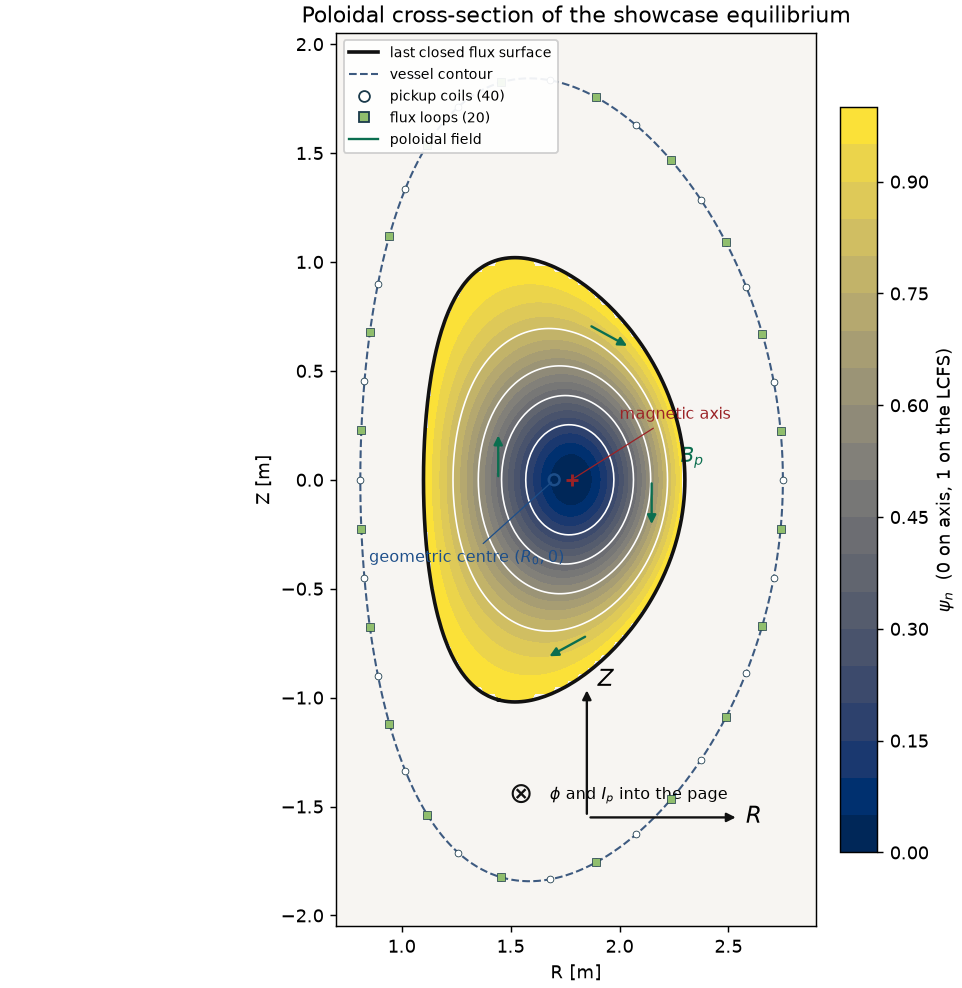
\includegraphics[width=0.78\textwidth]{tokamak_cross_section.png}
\caption[Poloidal cross-section of the showcase equilibrium]{Poloidal cross-section of the showcase equilibrium, solved on the shared fixed-boundary box \(R\in[0.80,2.76]\), \(Z\in[-1.90,1.90]\) at \(129\times 129\), with the synthetic vessel and sensors of \code{SensorSet.for_grid}. Read \(R\) to the right and \(Z\) upward. The symbol \(\otimes\) is \(\phi\), into the page, and it is also the direction of \(\Ip\). Colour is \(\psin\): dark at the axis, light at the edge. The black curve is the LCFS. The red cross is the magnetic axis and the open circle is the geometric centre \((R_{0},0)\); the gap between them is the Shafranov shift, outward. Green arrows are \(\mathbf{B}_{p}\) from \eqref{eq:Bcomp}. They run clockwise, the right-hand rule for a current into the page. The dashed curve is the vessel. Open circles mark the \(40\) pickup locations (each carries a tangential and a normal measurement) and green squares are the \(20\) flux loops. The Rogowski coil is the vessel loop, not an extra dot. The sensors sit well outside the plasma. That gap is why the inverse problem in \cref{ch:inverse} is hard: the diagnostic sees the field after it has fallen off, and many interior current distributions share nearly the same exterior.}
\label{fig:cross}
\end{figure}

\section*{Check your understanding}
\begin{enumerate}[label=\textbf{Q4.\arabic*.},leftmargin=2.4em]
\item Using \eqref{eq:Bcomp}, show that \(\mathbf{B}\cdot\grad\psi=0\) without expanding every term of \eqref{eq:Brep}.
\item The showcase axis value is \(\psi_{\mathrm{axis}}=0.358870\,\mathrm{Wb/rad}\). What is the physical flux through the horizontal circle at the axis, and why is there a factor \(2\pi\)?
\item Why does \(\mathbf{B}\cdot\grad p=0\), together with \(\mathbf{B}\cdot\grad\psi=0\) and axisymmetry, imply \(p=p(\psi)\) rather than an arbitrary function \(p(R,Z)\)?
\end{enumerate}

\begin{keyideas}
Axisymmetry reduces the equilibrium to the poloidal plane \((R,Z)\), with \(\phi\) and \(\Ip\) into the page. The field is \(\mathbf{B}=\grad\psi\times\grad\phi+F\grad\phi\), so \(B_{R}\) and \(B_{Z}\) are derivatives of \(\psi\) and \(B_{\phi}=F/R\). \(\psi\) is constant on field lines, and so is \(p\), hence \(p=p(\psi)\). The nested curves of constant \(\psi\) are the flux surfaces. The magnetic axis is their centre; the LCFS is the outer boundary, where this code sets \(\psi=0\).
\end{keyideas}

\chapter{The Grad--Shafranov equation}
\label{ch:gs}

\begin{objectives}
\begin{itemize}[leftmargin=1.2em]
\item Derive \(\Dstar\psi=-\mu_{0} R J_{\phi}\) from Amp\`ere's law and \eqref{eq:Bcomp}, including the expanded form used by the neural network.
\item Show that \(F=F(\psi)\), then obtain \(J_{\phi}=R p'+FF'/(\mu_{0} R)\) from the radial force balance.
\item State the Grad--Shafranov equation, the sign of \(FF'\) in this repository, and the difference between a fixed-boundary and a free-boundary problem.
\end{itemize}
\end{objectives}

Amp\`ere's law in steady state is \(\grad\times\mathbf{B}=\mu_{0}\mathbf{J}\), with \(\mu_{0}\) given in \eqref{eq:mu0}. The toroidal component, using the expressions for \(B_{R}\) and \(B_{Z}\) in \eqref{eq:Bcomp}, is the whole of this section's first half. The second half replaces \(J_{\phi}\) by the current that force balance demands.

\section{From Amp\`ere's law to \texorpdfstring{\(\Dstar\)}{Delta*}}

In cylindrical coordinates the toroidal component of the curl is
\begin{equation}
\label{eq:curlphi}
(\grad\times\mathbf{B})_{\phi}
=\frac{\partial B_{R}}{\partial Z}-\frac{\partial B_{Z}}{\partial R}.
\end{equation}
There is no extra \(1/R\) in this component: that factor appears in the radial and vertical components, which are used in the next section, and it is already sitting inside \(B_{R}\) and \(B_{Z}\). Substitute \eqref{eq:Bcomp}. The first term is immediate, because \(1/R\) does not depend on \(Z\):
\begin{equation}
\label{eq:dBr}
\frac{\partial B_{R}}{\partial Z}
=-\frac{1}{R}\frac{\partial^{2}\psi}{\partial Z^{2}}.
\end{equation}
The second term keeps the product rule inside the \(R\)-derivative, because \(1/R\) depends on \(R\):
\begin{equation}
\label{eq:dBz}
\frac{\partial B_{Z}}{\partial R}
=\frac{\partial}{\partial R}\!\left(\frac{1}{R}\frac{\partial\psi}{\partial R}\right).
\end{equation}
Amp\`ere's law \(\mu_{0} J_{\phi}=(\grad\times\mathbf{B})_{\phi}\) is therefore
\begin{equation}
\label{eq:Jphi-amp}
\mu_{0} J_{\phi}
=\frac{\partial B_{R}}{\partial Z}-\frac{\partial B_{Z}}{\partial R}
=-\frac{1}{R}\frac{\partial^{2}\psi}{\partial Z^{2}}
-\frac{\partial}{\partial R}\!\left(\frac{1}{R}\frac{\partial\psi}{\partial R}\right).
\end{equation}
Multiply through by \(-R\). The first term on the right becomes \(\partial^{2}\psi/\partial Z^{2}\). The second becomes
\[
R\frac{\partial}{\partial R}\!\left(\frac{1}{R}\frac{\partial\psi}{\partial R}\right).
\]
That combination is the operator the whole project calls \(\Dstar\):
\begin{equation}
\label{eq:dstar}
\Dstar\psi
\equiv
R\frac{\partial}{\partial R}\!\left(\frac{1}{R}\frac{\partial\psi}{\partial R}\right)
+\frac{\partial^{2}\psi}{\partial Z^{2}}
=-\mu_{0} R J_{\phi}.
\end{equation}
The finite-difference code uses this form, because it is a divergence of a flux and conserves current well on a grid.

Expand the \(R\)-derivative to see the form the physics-informed network uses. Let \(\partial_{R}\psi\) denote \(\partial\psi/\partial R\). Then
\begin{align}
R\frac{\partial}{\partial R}\!\left(R^{-1}\partial_{R}\psi\right)
&=R\Bigl(-R^{-2}\partial_{R}\psi+R^{-1}\partial_{R}^{2}\psi\Bigr)
=\partial_{R}^{2}\psi-\frac{1}{R}\partial_{R}\psi.
\label{eq:expand}
\end{align}
Hence
\begin{equation}
\label{eq:dstar-exp}
\Dstar\psi
=\frac{\partial^{2}\psi}{\partial R^{2}}
-\frac{1}{R}\frac{\partial\psi}{\partial R}
+\frac{\partial^{2}\psi}{\partial Z^{2}}
=-\mu_{0} R J_{\phi}.
\end{equation}
The two writings are the same identity. Automatic differentiation gives ordinary partial derivatives, so the network uses \eqref{eq:dstar-exp}. They agree for a smooth \(\psi\).

\section{\texorpdfstring{\(F\)}{F} is a flux function}

Equation~\eqref{eq:dstar} relates \(J_{\phi}\) to \(\psi\). Force balance relates \(J_{\phi}\) to \(p\) and \(F\). First, \(F\) has to be a flux function. The poloidal components of Amp\`ere's law are
\begin{equation}
\label{eq:JRJZ}
\mu_{0} J_{R}=-\frac{1}{R}\frac{\partial F}{\partial Z},
\qquad
\mu_{0} J_{Z}=\frac{1}{R}\frac{\partial F}{\partial R}.
\end{equation}
Since \(p=p(\psi)\) and \(\mathbf{J}\cdot\grad p=0\), the poloidal current is perpendicular to \(\grad\psi\) wherever \(p'(\psi)\neq 0\):
\begin{equation}
\label{eq:Jpol}
J_{R}\frac{\partial\psi}{\partial R}+J_{Z}\frac{\partial\psi}{\partial Z}=0.
\end{equation}
The prime will always mean a derivative with respect to \(\psi\), not \(R\). Substitute \(J_{R}\) and \(J_{Z}\) from \eqref{eq:JRJZ}:
\begin{equation}
\label{eq:Fparallel}
-\frac{\partial F}{\partial Z}\frac{\partial\psi}{\partial R}
+\frac{\partial F}{\partial R}\frac{\partial\psi}{\partial Z}
=0.
\end{equation}
The \(\mu_{0} R\) factor cancelled. Equation~\eqref{eq:Fparallel} says that the poloidal gradients of \(F\) and \(\psi\) are parallel: their cross product in the \((R,Z)\) plane vanishes. Wherever \(\grad\psi\neq\mathbf{0}\), \(F\) is constant on the curves of constant \(\psi\). So
\begin{equation}
\label{eq:Fpsi}
F=F(\psi).
\end{equation}
On the magnetic axis \(\grad\psi=\mathbf{0}\) and the argument does not apply, but \(F\) is already determined by continuity from the surfaces around the axis.

\section{The toroidal current from force balance}

Now the radial component of \(\mathbf{J}\times\mathbf{B}=\grad p\). In the right-handed basis,
\begin{equation}
\label{eq:JxBR}
(\mathbf{J}\times\mathbf{B})_{R}=J_{\phi} B_{Z}-J_{Z} B_{\phi},
\end{equation}
and \((\grad p)_{R}=p'(\psi)\,\partial\psi/\partial R\). From \eqref{eq:Fpsi} and \eqref{eq:JRJZ},
\begin{equation}
\label{eq:JZ}
\frac{\partial F}{\partial R}=F'(\psi)\frac{\partial\psi}{\partial R},
\qquad
J_{Z}=F'(\psi)\,\frac{1}{\mu_{0} R}\,\frac{\partial\psi}{\partial R}.
\end{equation}
Insert \(B_{Z}=(1/R)\,\partial\psi/\partial R\) and \(B_{\phi}=F/R\) into \eqref{eq:JxBR}:
\begin{equation}
\label{eq:radial-balance}
J_{\phi}\cdot\frac{1}{R}\frac{\partial\psi}{\partial R}
-J_{Z}\cdot\frac{F}{R}
=p'(\psi)\frac{\partial\psi}{\partial R}.
\end{equation}
The second term on the left contains another \(\partial\psi/\partial R\), by \eqref{eq:JZ}. Away from the axis that factor is not identically zero, so divide the whole equation by \(\partial\psi/\partial R\):
\begin{equation}
\label{eq:divide}
\frac{J_{\phi}}{R}
-\frac{F F'(\psi)}{\mu_{0} R^{2}}
=p'(\psi).
\end{equation}
Multiply through by \(R\):
\begin{equation}
\label{eq:Jphi}
J_{\phi}
=R\,p'(\psi)+\frac{F F'(\psi)}{\mu_{0} R}.
\end{equation}
Each term has a job. The piece \(R p'(\psi)\) is the toroidal current that \(\mathbf{J}\times\mathbf{B}\) needs in order to hold up \(\grad p\). The piece \(FF'(\psi)/(\mu_{0} R)\) is the toroidal current that comes with a poloidal current, and the poloidal current is what changes the toroidal field from its vacuum value.

\section{The equation}

Put \eqref{eq:Jphi} into \(\Dstar\psi=-\mu_{0} R J_{\phi}\). You obtain the Grad--Shafranov equation.

\begin{gsbox}
\begin{equation}
\label{eq:gs}
\Dstar\psi=-\mu_{0} R^{2}\, p'(\psi)-F(\psi)\,F'(\psi).
\end{equation}
\end{gsbox}

Each term on the right-hand side is \(-\mu_{0} R\) times one piece of \(J_{\phi}\). In the sign convention of this repository, \(\psi\) is largest on the magnetic axis when \(\Ip>0\), and \(p'(\psi)>0\) means pressure rises toward the axis. \(FF'>0\) then means \(F\) itself rises toward the axis: \(B_{\phi}\) in the core is stronger than the vacuum toroidal field \(R_{0} B_{0}/R\). That is a paramagnetic equilibrium. A diamagnetic equilibrium, with \(F\) smaller on axis, would need \(FF'<0\). The profile family in \cref{ch:code} never produces that sign.

The equation is elliptic for the same reason a Poisson equation is elliptic: \(\Dstar\) is a second-order operator with the sign of the Laplacian, and with \(\psi\) fixed on a closed boundary the solution is unique for a given right-hand side. It is nonlinear because \(p'\) and \(FF'\) depend on the unknown \(\psi\). You cannot write the right-hand side until you know the surfaces. The practical algorithm is Picard iteration: guess \(\psi\), evaluate the current, solve the linear elliptic equation, under-relax, and repeat. The discrete version is in \cref{ch:code}.

Two boundary-value problems sit on this equation. In the fixed-boundary problem the shape of the LCFS is given, \(\psi\) is prescribed there (zero, in this code), and the profile functions are given. The unknown is \(\psi\) inside. In the free-boundary problem the coils are given and the LCFS is not. The plasma boundary becomes the surface that passes through an X-point, or that is tangent to a limiter, and outside the plasma one solves \(\Dstar\psi=0\) together with the coil fields. Almost every learned model in this repository is fixed-boundary. The FreeGS dataset in \cref{ch:code} is the exception.

\begin{worked}{Density from the axis pressure}
\label{ex:density}
The showcase equilibrium of \cref{ch:figures} has an axis pressure of \(100.8\,\mathrm{kPa}\). The equilibrium itself carries no temperature. A density scale is only a conversion of those pascals, using the design temperature from \cref{ch:bottle}.

Take the pressure as \(n_{e} k T_{e}+n_{i} k T_{i}\) with \(n_{e}=n_{i}\) and \(T_{e}=T_{i}=\qty{10}{\kilo\electronvolt}\). Then \(p=2 n_{e} k T\), and the energy \(k T\) corresponding to \(\qty{10}{\kilo\electronvolt}\) is
\[
k T=1.602\times 10^{-15}\,\mathrm{J},
\]
the conversion stated with this example in the source note (\(1\,\mathrm{eV}=1.602\times 10^{-19}\,\mathrm{J}\), times \(10^{4}\)). So
\begin{align*}
n_{e}
&=\frac{p}{2 k T}
=\frac{100.8\times 10^{3}}{2\times 1.602\times 10^{-15}}
=\frac{1.008\times 10^{5}}{3.204\times 10^{-15}}\\
&=3.146\times 10^{19}\,\mathrm{m}^{-3},
\end{align*}
which rounds to the reported \(3.15\times 10^{19}\,\mathrm{m}^{-3}\). Changing the assumed temperature changes \(n_{e}\) in inverse proportion. Nothing in the Grad--Shafranov solve knows which temperature you assumed.
\end{worked}

\begin{worked}{Poloidal field from Amp\`ere's law}
\label{ex:bp}
The combination \(\mu_{0}\Ip/\ell\) is the characteristic poloidal field from Amp\`ere's law around the boundary. If \(B_{p}\) were constant in magnitude along the LCFS, \(\oint\mathbf{B}\cdot d\mathbf{l}=\mu_{0}\Ip\) would say \(B_{p}\ell=\mu_{0}\Ip\). The length \(\ell\) is not printed in the source note. It is computed here from the same polyline the figure code uses.

On the showcase plasma (\(\Ip=\qty{1}{\mega\ampere}\), \(R_{0}=\qty{1.7}{\metre}\), \(a=\qty{0.6}{\metre}\), \(\kappa=1.7\), \(\delta=0.3\), \(\beta_{0}=0.5\), \(\alpha=1\), \(\gamma=2\), \(B_{0}=\qty{2}{\tesla}\)), the default \(129\times 129\) covering grid of \code{eval.visualize} is \(R\) from \(0.823\) to \(2.577\,\mathrm{m}\) and \(Z\) from \(-1.458\) to \(1.458\,\mathrm{m}\). That is the grid behind \code{equilibrium.png}. Calling \code{solve_fixed_boundary} on it and summing the segment lengths of \code{eval.visualize._lcfs_polyline} gives
\begin{equation}
\label{eq:ell}
\ell=5.190240\,\mathrm{m}.
\end{equation}
The axis flux on that solve is \(0.358870\,\mathrm{Wb/rad}\), matching the value quoted above, so this is the same equilibrium. Then
\begin{align}
\mu_{0}\Ip
&=(4\pi\times 10^{-7})(1.000\times 10^{6})
=1.256637\,\mathrm{T\,m},
\label{eq:mu0Ip}\\
B_{p}^{\mathrm{char}}
&=\frac{\mu_{0}\Ip}{\ell}
=\frac{1.256637}{5.190240}
=0.24212\,\mathrm{T}.
\label{eq:bpchar}
\end{align}
The poloidal field that holds a one-megaampere plasma of this perimeter is a quarter of a tesla, while \(B_{0}=\qty{2}{\tesla}\). The toroidal field is an order of magnitude larger. That is why the toroidal magnetic pressure dominates, as the tension-and-pressure split suggested.

The same solve reports \(\beta_{p}=0.540\). The figure code defines
\begin{equation}
\label{eq:betap-def}
\beta_{p}=\frac{2\langle p\rangle\,\ell^{2}}{\mu_{0}\Ip^{2}}
=\frac{\langle p\rangle}{B_{p}^{2}/(2\mu_{0})},
\end{equation}
with \(\langle p\rangle\) the area average of the pressure on the plasma mask. On this grid that average is \(\langle p\rangle=1.2587\times 10^{4}\,\mathrm{Pa}=12.587\,\mathrm{kPa}\), again from the project's pressure routine, not from a saved JSON file. The magnetic pressure of the characteristic poloidal field is
\begin{equation}
\label{eq:magp}
\frac{(B_{p}^{\mathrm{char}})^{2}}{2\mu_{0}}
=\frac{(0.24212)^{2}}{2\times 1.256637\times 10^{-6}}
=2.332\times 10^{4}\,\mathrm{Pa}
=23.32\,\mathrm{kPa}.
\end{equation}
The ratio \(12.587/23.32=0.540\) reproduces the reported \(\beta_{p}\). The check is only arithmetic: once \(\ell\) and \(\langle p\rangle\) are taken from the solve, \(\beta_{p}\) is not an independent measurement.
\end{worked}

\section*{Check your understanding}
\begin{enumerate}[label=\textbf{Q5.\arabic*.},leftmargin=2.4em]
\item Why does the network evaluate \(\partial_{R}^{2}\psi-R^{-1}\partial_{R}\psi+\partial_{Z}^{2}\psi\) while the solver evaluates \(R\partial_{R}(R^{-1}\partial_{R}\psi)+\partial_{Z}^{2}\psi\)? When do the two disagree?
\item Starting from \(J_{\phi}=R p'+FF'/(\mu_{0} R)\), write the two-line substitution that produces \eqref{eq:gs}.
\item In this sign convention, what does \(FF'>0\) mean for \(B_{\phi}\) on axis, and does the project's profile family ever give the other sign?
\end{enumerate}

\begin{keyideas}
Amp\`ere's law turns \(\psi\) into \(J_{\phi}\) through the operator \(\Dstar\). Force balance turns \(p(\psi)\) and \(F(\psi)\) into that same \(J_{\phi}\). Eliminating \(J_{\phi}\) produces \(\Dstar\psi=-\mu_{0} R^{2} p'-FF'\). The equation is an elliptic boundary-value problem, nonlinear because the surfaces that define \(p'\) and \(FF'\) are unknown until \(\psi\) is known. This repository's profiles are paramagnetic: \(FF'>0\). Fixed-boundary problems prescribe the LCFS; free-boundary problems prescribe the coils.
\end{keyideas}


\chapter{Safety factor, shape, and beta}
\label{ch:quantities}

\begin{objectives}
\begin{itemize}[leftmargin=1.2em]
\item Define the Shafranov shift, \(\psin\), and \(q(\psin)\), and say why the code reports \(q_{95}\) rather than \(q\) on the boundary.
\item Separate the Kruskal--Shafranov edge condition from the \(m=1\) internal kink.
\item Read elongation, triangularity, \(\beta_{p}\), and \(l_{i}\) off the definitions, and state which combination external magnetics can see.
\end{itemize}
\end{objectives}

\section{The shift of the axis}

The magnetic axis is the extremum of \(\psi\) inside the plasma. Here that extremum is a maximum, \(\psi_{\mathrm{axis}}>0\), and it sits near the midplane. It is not at the geometric centre \((R_{0},0)\). The outward displacement
\begin{equation}
\label{eq:shift}
\Delta_{s}=R_{\mathrm{axis}}-R_{0}
\end{equation}
is the Shafranov shift. A toroidal current loop wants to expand, like any current-carrying hoop in its own field, and plasma pressure pushes the same way, so the nest of surfaces is squeezed outward. On the showcase equilibrium drawn in \cref{fig:equilibrium}, \(\Delta_{s}=+0.0799\,\mathrm{m}\) on a minor radius \(a=\qty{0.60}{\metre}\).

\section{Normalized flux}

The LCFS is the boundary curve. Inside it the surfaces are closed and nested. The normalized flux used everywhere in the code is
\begin{equation}
\label{eq:psin}
\psin=\frac{\psi-\psi_{\mathrm{axis}}}{\psi_{\mathrm{boundary}}-\psi_{\mathrm{axis}}}.
\end{equation}
With \(\psi_{\mathrm{boundary}}=0\) and \(\psi_{\mathrm{axis}}>0\) this is \(0\) on the axis and \(1\) on the LCFS. Profiles are plotted against \(\psin\) so that plasmas of different size and current can be compared. Do not confuse \(\psin\) with the analytic Solov'ev flux \(\psibar\) of \cref{ch:code}. \(\psibar\) is negative inside the plasma. \(\psin\) is a shape coordinate in \([0,1]\).

\section{Safety factor}

The safety factor measures the twist introduced in \cref{ch:bottle}. Follow a field line until it has gone once around the short way. The number of long-way turns it made is \(q\). On a surface of constant \(\psi\),
\begin{equation}
\label{eq:q}
q(\psin)=\frac{F}{2\pi}\oint\frac{\mathrm{d}l}{R^{2} B_{p}},
\end{equation}
where the integral is once around the poloidal contour, \(B_{p}=\lvert\grad\psi\rvert/R\) is the poloidal field strength, and \(\mathrm{d}l\) is arc length. \(F\) comes out of the integral because it is constant on the surface. Large \(q\) means little twist. The code evaluates this in \code{eval/metrics.py} by drawing the contour on a refined grid and integrating with segment midpoints. It refuses \(\psin=0\) and \(\psin=1\), where \(B_{p}\) vanishes or the contour degenerates, and reports \(q_{95}=q(0.95)\) instead of an edge value. That convention is the usual one on real devices as well: at a diverted X-point \(B_{p}\to 0\) and \(q\) diverges, so the value at \(95\%\) of the flux is the number people quote.

Two round numbers are worth remembering, as stability facts rather than as something this code computes. The Kruskal--Shafranov limit concerns the edge: the external kink is unstable if \(q\) at the boundary drops below \(1\), and in practice tokamaks operate with \(q_{95}\) around \(3\) or higher, partly to keep the \(q=2\) surface (where the \(m=2\), \(n=1\) mode lives) away from the edge. In the core, a \(q=1\) surface inside the plasma allows the \(m=1\) internal kink, which in real tokamaks shows up as periodic ``sawtooth'' crashes of the central temperature. Many tokamaks run with \(q_{0}\) slightly below \(1\) and tolerate sawteeth, but it is a real effect. The showcase equilibrium in \cref{fig:equilibrium} has \(q(0.05)=0.662\) and \(q_{95}=4.955\): the edge is comfortably safe, and the core would be sawtoothing. Nothing in the dataset generator rejects a solution for its \(q\) profile. These are equilibria, not stability-checked scenarios.

The edge condition and the core condition are different statements. Kruskal--Shafranov is a condition on \(q\) at the boundary. The sawtooth is what you get when \(q\) passes through \(1\) inside the plasma, even if \(q_{95}\) is several times larger. The showcase has both: a safe edge and an unsafe core.

\section{Shape}

The shape of the boundary is described by three numbers. \(R_{0}\) is the major radius of the geometric centre and \(a\) is the minor radius, half the width of the cross-section. The inverse aspect ratio is \(\varepsilon=a/R_{0}\). Elongation \(\kappa\) is the height divided by the width: \(\kappa=1\) is circular, and the showcase uses \(\kappa=1.7\). Triangularity \(\delta\) pulls the top and bottom tips inward toward the axis. The curve the solver aims at is the up--down symmetric Miller shape
\begin{equation}
\label{eq:miller}
R=R_{0}+a\cos\bigl(\tau+\arcsin(\delta)\sin\tau\bigr),
\qquad
Z=\kappa a\sin\tau,
\end{equation}
with \(\tau\) running from \(0\) to \(2\pi\). The boundary that is actually imposed is not this curve pointwise. It is the zero contour of a Solov'ev solution that is required to pass through the inner equator, the outer equator, and the top of the Miller curve, and to match the curvature there (Cerfon and Freidberg). For the shapes in the dataset the two curves are close. Panel~(d) of \cref{fig:profiles} shows the Miller targets.

\section{Beta and internal inductance}

Plasma beta is the ratio of plasma pressure to magnetic pressure, \(\beta=2\mu_{0}\langle p\rangle/B^{2}\). Poloidal beta \(\beta_{p}\) uses the poloidal field, which is the field the plasma current itself produces. The figure code defines \eqref{eq:betap-def}, with \(\ell\) the length of the LCFS. On the showcase plasma \(\beta_{p}=0.540\). That number is not the input \(\beta_{0}\). \Cref{ch:code} explains \(\beta_{0}\); it is a mix parameter in the current profile. They happen to be numerically close for that one plasma. \Cref{ex:bp} is the arithmetic that connects \(\beta_{p}=0.540\) to \(\mu_{0}\Ip/\ell\).

Internal inductance \(l_{i}\) measures how peaked the toroidal current is, through the magnetic energy stored in the poloidal field inside the plasma. A centrally peaked current has large \(l_{i}\). The code never evaluates \(l_{i}\). It matters for the inverse problem because, for a circular large-aspect-ratio plasma, external magnetic measurements determine the sum \(\beta_{p}+l_{i}/2\) and not the two terms separately (Shafranov; the shaped-plasma version is in Lao et al., the EFIT paper). \Cref{ch:inverse} is that fact, measured on this dataset.

\begin{figure}[p]
\centering
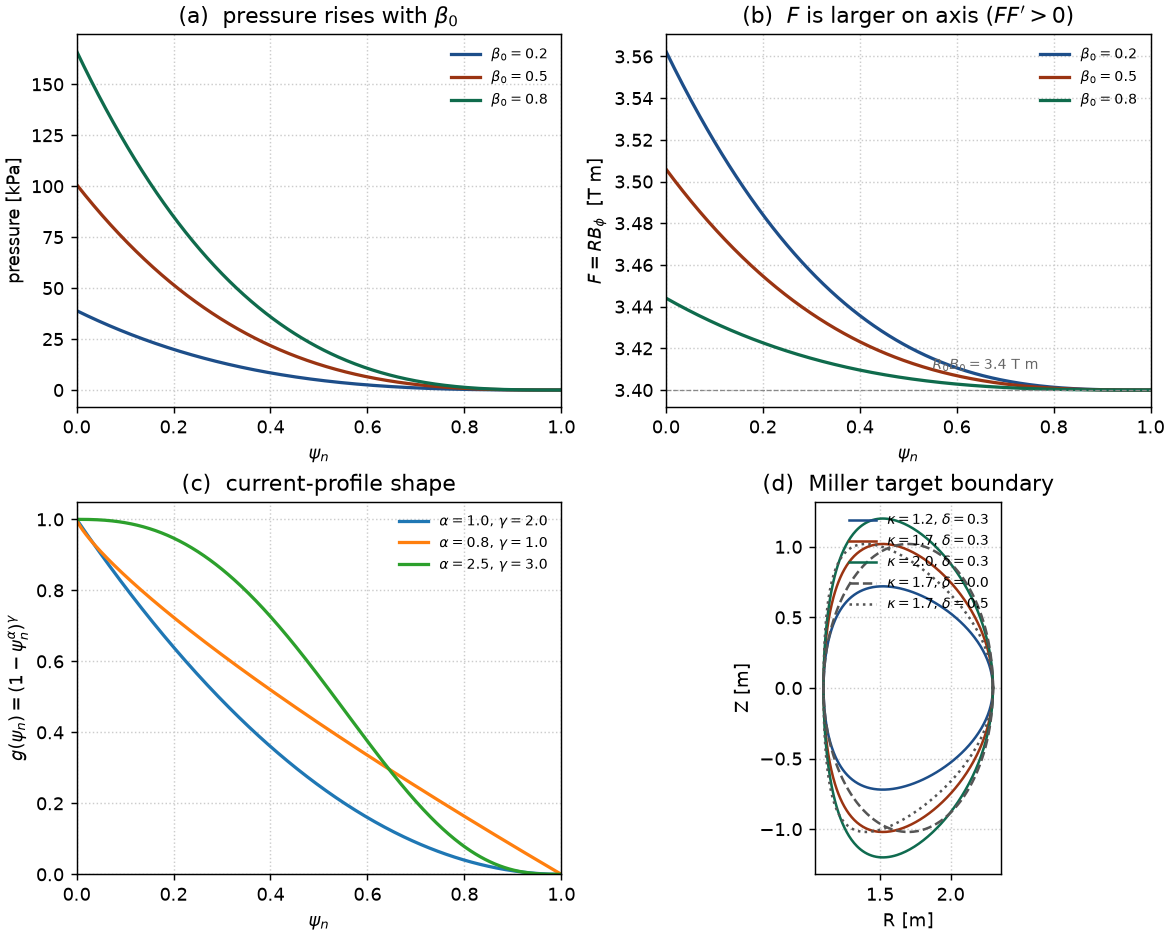
\includegraphics[width=\textwidth]{profiles_and_shapes.png}
\caption[Pressure, toroidal field, profile shape, and Miller targets]{Profile and shape parameters for the showcase geometry, computed with the project's solver. Panel~(a) is pressure against \(\psin\) at three values of \(\beta_{0}\), with \(\Ip\), \(B_{0}\), and the shape held fixed. Axis pressure rises from \(\qty{39.0}{\kilo\pascal}\) at \(\beta_{0}=0.2\) to \(\qty{101}{\kilo\pascal}\) at \(\beta_{0}=0.5\) and \(\qty{166}{\kilo\pascal}\) at \(\beta_{0}=0.8\). Panel~(b) is \(F=RB_{\phi}\). Every curve ends at \(R_{0}B_{0}=\qty{3.40}{\tesla\metre}\) and is larger on axis: \(3.563\), \(3.506\), and \(3.444\,\mathrm{T\,m}\). Raising \(\beta_{0}\) raises the pressure and shrinks the paramagnetic bump, because \((1-\beta_{0})\) multiplies \(FF'\). The Shafranov shift on this grid grows with \(\beta_{0}\): \(\qty{0.054}{\metre}\), \(\qty{0.080}{\metre}\), \(\qty{0.104}{\metre}\). Panel~(c) is only the shape function \(g(\psin)\), so it does not require a solve. Panel~(d) is the Miller target at fixed \(R_{0}=\qty{1.7}{\metre}\) and \(a=\qty{0.6}{\metre}\). Increasing \(\kappa\) stretches the cross-section vertically. Increasing \(\delta\) pulls the tips toward smaller \(R\) and makes the D shape.}
\label{fig:profiles}
\end{figure}

\begin{figure}[p]
\centering
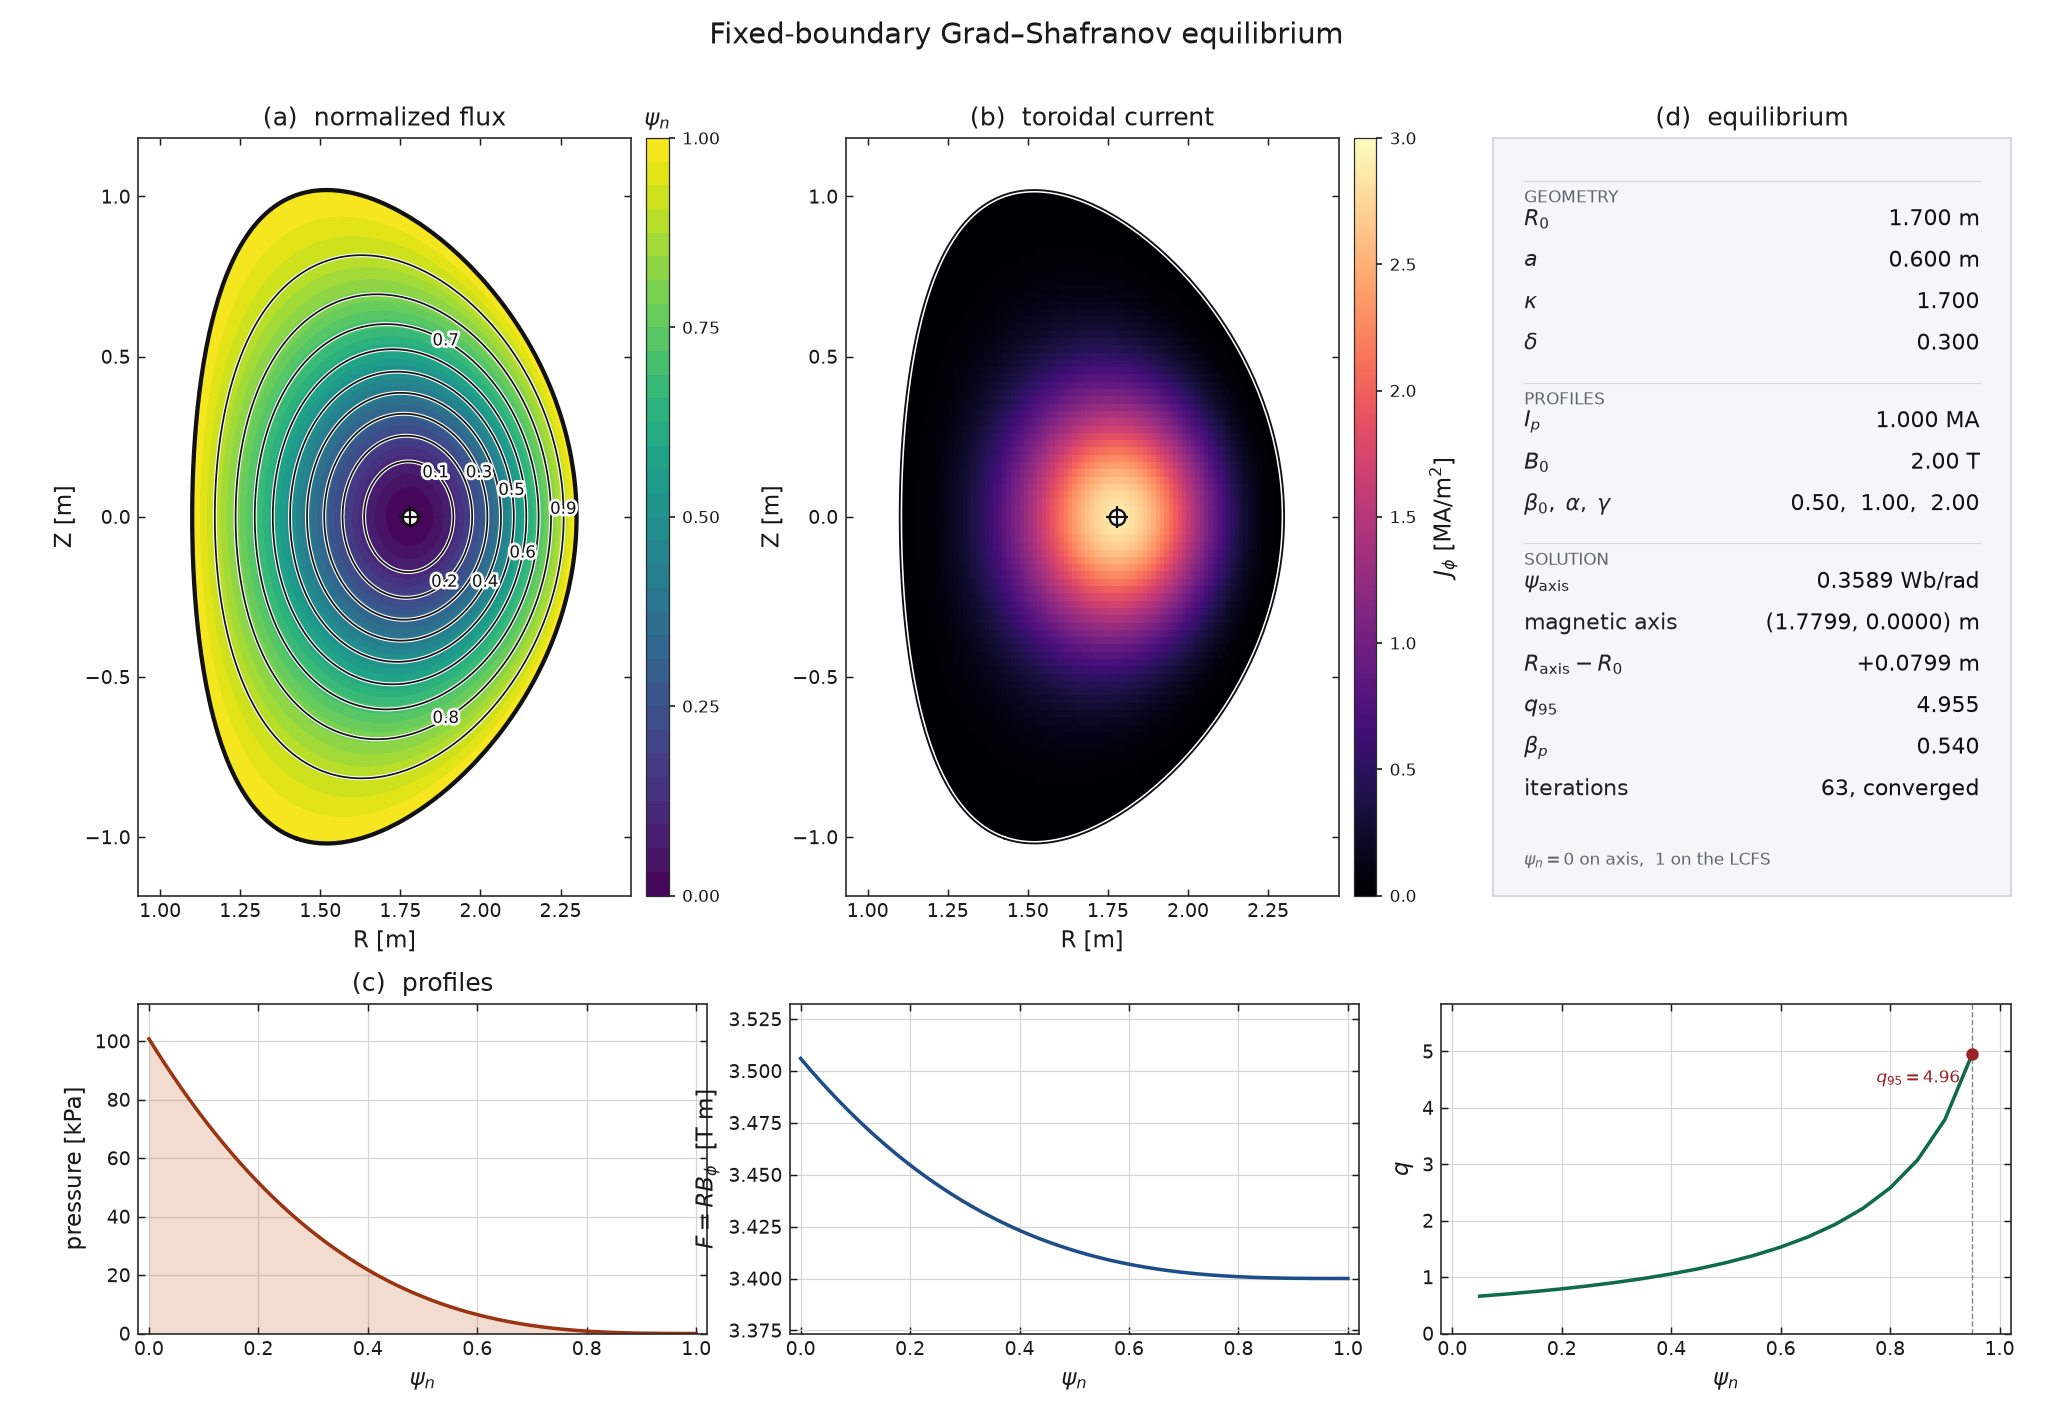
\includegraphics[width=\textwidth]{equilibrium.png}
\caption[Showcase equilibrium from the finite-difference solver]{Showcase equilibrium from the finite-difference solver, the default case of \code{eval.visualize}, on the \(129^{2}\) covering grid \(R\) from \(0.823\) to \(2.577\,\mathrm{m}\) and \(Z\) from \(-1.458\) to \(1.458\,\mathrm{m}\). Panel~(a): \(\psin\) with nine labelled surfaces from \(0.1\) to \(0.9\), the LCFS in black, and the axis marked. The surfaces are up--down symmetric and shifted outward. Panel~(b): \(J_{\phi}\) in \(\mathrm{MA/m}^{2}\), clipped to the LCFS. The peak is \(\qty{2.87}{\mega\ampere\per\square\metre}\), so the colour scale tops out at \(3\). The current is peaked on axis because \(g=(1-\psin)^{2}\) for \(\alpha=1\), \(\gamma=2\). Panel~(c): pressure falls from \(\qty{100.8}{\kilo\pascal}\) on axis to zero at the edge (the density estimate is \cref{ex:density}); \(F\) falls from \(3.506\,\mathrm{T\,m}\) on axis to \(3.400\,\mathrm{T\,m}\) at the edge, a \(3\%\) paramagnetic rise toward the core, on a zoomed vertical axis; \(q\) rises from \(0.662\) at \(\psin=0.05\) to \(q_{95}=4.955\). The edge satisfies the Kruskal--Shafranov condition; the core is below \(q=1\) and would be sawtoothing. Panel~(d): \(\psi_{\mathrm{axis}}=0.3589\,\mathrm{Wb/rad}\), axis at \((1.7799,0)\,\mathrm{m}\), shift \(+0.0799\,\mathrm{m}\), \(\beta_{p}=0.540\), and \(63\) iterations. The integral of \(J_{\phi}\) recovers \(\Ip=\qty{1.000}{\mega\ampere}\), and the discrete Grad--Shafranov residual is \(1.50\times 10^{-8}\).}
\label{fig:equilibrium}
\end{figure}

\section*{Check your understanding}
\begin{enumerate}[label=\textbf{Q6.\arabic*.},leftmargin=2.4em]
\item The showcase has \(q(0.05)=0.662\) and \(q_{95}=4.955\). Which of those numbers is the Kruskal--Shafranov diagnostic, and which one is the sawtooth diagnostic?
\item Compute \(\varepsilon=a/R_{0}\) for the showcase values \(a=\qty{0.60}{\metre}\) and \(R_{0}=\qty{1.7}{\metre}\).
\item Why can external magnetics determine \(\beta_{p}+l_{i}/2\) and still fail to determine the current profile?
\end{enumerate}

\begin{keyideas}
The magnetic axis sits outward of the geometric centre by the Shafranov shift. \(\psin\) runs from \(0\) on axis to \(1\) on the LCFS and is the coordinate for profiles. The safety factor \(q\) counts toroidal turns per poloidal turn; the code quotes \(q_{95}\). Kruskal--Shafranov is an edge condition (\(q\) at the boundary below \(1\) is unstable). A \(q=1\) surface in the core allows the \(m=1\) internal kink and sawteeth. \(\kappa\) and \(\delta\) set the Miller target. \(\beta_{p}\) is not \(\beta_{0}\). External coils and probes see \(\beta_{p}+l_{i}/2\), not the two pieces.
\end{keyideas}

\chapter{Why a fast equilibrium is worth having}
\label{ch:speed}

\begin{objectives}
\begin{itemize}[leftmargin=1.2em]
\item Name two operational reasons a tokamak recomputes equilibria, and the time scale of vertical instability.
\item Quote the cost of one \(65\times 65\) solve in this repository, and the cost of one network evaluation.
\item State the honest conclusion: speed on this grid is not the reason to prefer the learned map.
\end{itemize}
\end{objectives}

A tokamak control system recomputes, or at least corrects, the equilibrium many times a second. Vertical position control in particular has to be fast: the plasma can be unstable to a vertical drift on a millisecond time scale, and the coils have to push back. Between shots, and in scenario design, one also wants hundreds or thousands of equilibria: scans in shape, current, and pressure. Equilibrium reconstruction, the EFIT procedure of Lao et al.\ (1985), solves an inverse Grad--Shafranov problem so that the synthetic magnetic signals match the measured ones, often with extra internal data.

The finite-difference solve in this repository is already cheap. One nonlinear \(65\times 65\) equilibrium takes \(\qty{44.3}{\milli\second}\) on the machine that produced \code{outputs/compare/speed.json}. A trained network evaluates one equilibrium in about \(\qtyrange{1}{3}{\milli\second}\), and the best surrogate evaluates a batch of \(500\) in \(\qty{273}{\milli\second}\), which is \(\qty{0.55}{\milli\second}\) each. The honest reading is that a \(65\times 65\) fixed-boundary Picard solve does not need to be replaced for speed. The interesting uses of the learned maps are elsewhere: a batch scan, a free-boundary solve that is much more expensive than this one, and the inverse problem, where the network is a fast guess inside a family it has seen. Degrave et al.\ (Nature, 2022) showed that a learned controller can hold the shape and position of the TCV tokamak; that work is about control, not about solving Grad--Shafranov, but it is the reason millisecond magnetic models are taken seriously.

What a network cannot do is invent information. The inverse experiments in \cref{ch:inverse} are a measurement of how much of \(\psi\) the external sensors actually contain.

\begin{figure}[htbp]
\centering
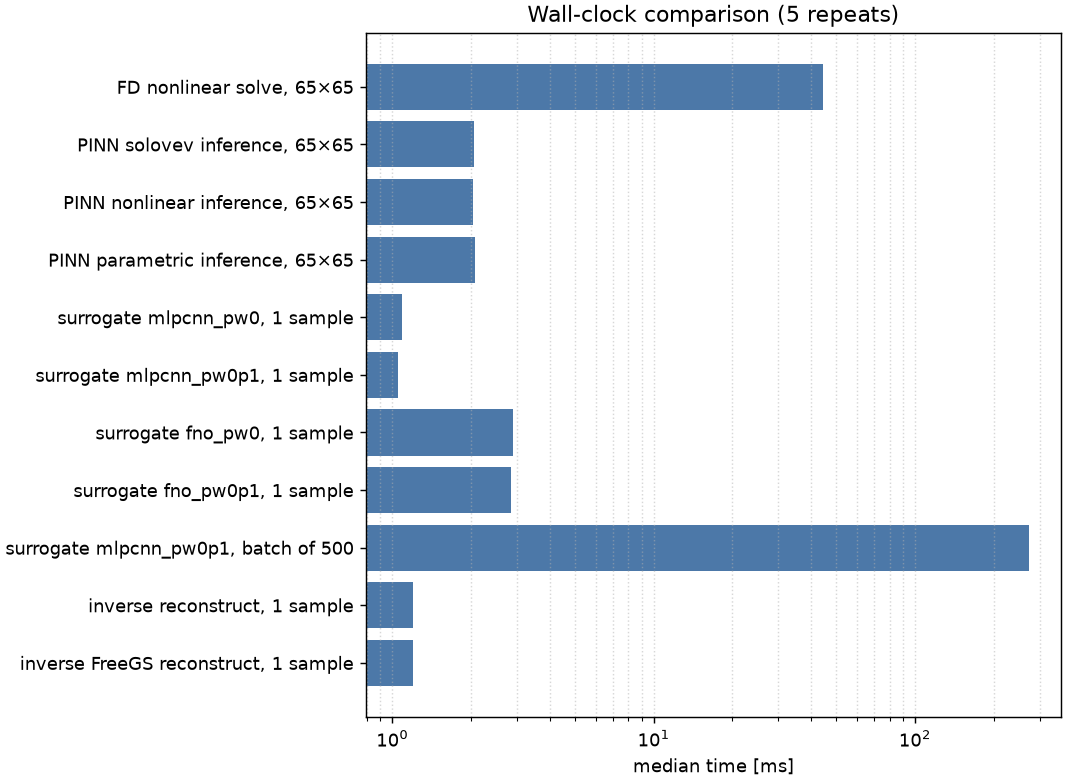
\includegraphics[width=0.78\textwidth]{speed.png}
\caption[Wall-clock time of the solver and the networks]{Wall-clock comparison from \code{outputs/compare/speed.json}: the median of five calls after one warm-up, with PyTorch limited to two threads. The nonlinear solve is the long bar, \(\qty{44.32}{\milli\second}\) for the showcase equilibrium at \(65\times 65\). Every network forward pass is a few milliseconds (the best surrogate, \code{mlpcnn_pw0p1}, takes \(\qty{1.05}{\milli\second}\) for one sample). The batch of \(500\) is the one network bar that reaches hundreds of milliseconds (\(\qty{273.42}{\milli\second}\)), and per plasma it is the cheapest of all (\(\qty{0.55}{\milli\second}\)).}
\label{fig:speed}
\end{figure}

\section*{Check your understanding}
\begin{enumerate}[label=\textbf{Q7.\arabic*.},leftmargin=2.4em]
\item A single fixed-boundary equilibrium on this \(65\times 65\) grid costs \(\qty{44.3}{\milli\second}\). Why is that not, by itself, a reason to replace the solver with a network?
\item The batch of \(500\) costs \(\qty{273}{\milli\second}\). What is the cost per plasma, and which use of the model does that number support?
\item Degrave et al.\ (2022) is often cited next to learned equilibrium models. What did that paper actually demonstrate?
\end{enumerate}

\begin{keyideas}
Control, scenario scans, and EFIT reconstruction all call an equilibrium solve repeatedly. Vertical control lives on a millisecond scale. Here one nonlinear \(65\times 65\) solve takes \(\qty{44.3}{\milli\second}\) and one network evaluation takes about \(\qtyrange{1}{3}{\milli\second}\). The batch is where the surrogate is actually cheaper. A network cannot add information the sensors do not contain.
\end{keyideas}

\chapter{Machine learning, in the amount you need}
\label{ch:ml}

\begin{objectives}
\begin{itemize}[leftmargin=1.2em]
\item Describe a neural network as a parameterized map, a loss as an energy, and gradient descent as a descent on that energy.
\item Separate a training set, a validation set, a test set, and an out-of-distribution test.
\item Say what a CNN, an FNO, and a PINN each change about that picture, and define relative \(L^{2}\) and \(R^{2}\).
\end{itemize}
\end{objectives}

The models in the next three chapters are not a new physical theory. They are function fits. This chapter names the pieces, using analogies that already appear in mechanics and in numerical PDE methods. The precise architectures and the numbers they achieved are later.

\section{A parameterized function}

A neural network, for everything this project does, is a function
\begin{equation}
\label{eq:nn}
\mathbf{y}=f(\mathbf{x};\theta)
\end{equation}
with a fixed recipe and a long list of adjustable numbers \(\theta\), the weights. In the surrogate, \(\mathbf{x}\) is nine equilibrium parameters and \(\mathbf{y}\) is \(\psi\) on the grid. In the physics-informed network, \(\mathbf{x}\) is the point \((R,Z)\) and \(\mathbf{y}\) is the scalar \(\psi\). The recipe is a composition of affine maps and a simple nonlinearity. For a multilayer perceptron (MLP), one layer is
\begin{equation}
\label{eq:layer}
\mathbf{h}_{\ell+1}=\sigma(W_{\ell}\mathbf{h}_{\ell}+\mathbf{b}_{\ell}),
\end{equation}
with \(\sigma\) applied componentwise. The network in the physics-informed runs uses \(\sigma=\tanh\). There is no claim that \(\tanh\) is physical. It is a smooth function whose derivative does not vanish at the origin, which matters because the training signal is that derivative.

Think of \(\theta\) as the coefficients in a trial function, the way a Rayleigh--Ritz calculation writes a field as a sum of modes with unknown amplitudes. The difference is practical, not philosophical: there are \(10^{5}\) coefficients, the basis is defined implicitly by \eqref{eq:layer}, and the coefficients are chosen by descending a scalar loss rather than by solving a linear Galerkin system.

\section{Loss, descent, and Adam}

Training means choosing \(\theta\) to make a scalar loss \(L(\theta)\) small. \(L\) is an energy. For a supervised fit it is a sum of squared errors between \(f(\mathbf{x};\theta)\) and a known target. For a physics-informed network it is the squared residual of \eqref{eq:gs}, plus a penalty for missing the boundary condition. Minimizing \(L\) is the same kind of act as minimizing a potential. The gradient \(\grad_{\theta} L\) points uphill in weight space.

Gradient descent takes a step downhill,
\begin{equation}
\label{eq:gd}
\theta\leftarrow\theta-\eta\,\grad_{\theta} L,
\end{equation}
with learning rate \(\eta\). It is steepest descent. Plain steepest descent on a long, narrow valley oscillates across the valley and crawls along it. Adam (Kingma and Ba, 2015) is the optimizer used for the first stage of every training run here. It keeps a running average of the gradient, which is momentum: a heavy particle that does not reverse at every wiggle. It also keeps a running average of the squared gradient and divides by its square root, so coordinates that have always been steep get a smaller step. The details of the two averages are in the paper. What you need is that Adam is still a descent method on \(L\), with an adaptive step, and that it is not a symplectic integrator of a physical Hamiltonian. After a few hundred Adam steps the physics-informed runs switch to L-BFGS, a quasi-Newton method. Quasi-Newton methods build an approximate Hessian and take a step closer to the Newton step for \(\grad L=\mathbf{0}\). They are the right tool once the weights are near a minimum and the loss is smooth, which is why they appear second.

A physics penalty added to \(L\) is regularization in the same sense as a bending energy. You add a term that is large when the solution has a defect you care about, here a large Grad--Shafranov residual, and you accept a slightly worse fit to the original target if the defect gets much smaller. \Cref{ch:surrogate} is the measurement of that trade.

\section{Splits, overfitting, and extrapolation}

The supervised models are fit to a finite list of solved equilibria. That list is split into a training set, a validation set, and a test set: \(4000\), \(500\), and \(500\) for the fixed-boundary file. The training set is the only data that enter \(L\). The validation set is a held-out diagnostic used to decide when to stop and which of a few settings to keep. The test set is touched once, at the end. If you tune on the test set, it stops being a measurement.

Overfitting is what happens when \(f(\mathbf{x};\theta)\) memorizes the training examples, including whatever noise or discrete quirk they carry, and then misses a new draw from the same distribution. The symptom is a training loss far below the validation loss. The inverse model in \cref{ch:inverse} does not show that symptom: its training, validation, and test errors sit on top of each other. A model can also fail without overfitting. It can be incapable of representing the target, or the target can be ambiguous. The inverse problem is the second kind. The sensors do not determine \(\psi\), so no architecture, trained for longer, will drive the error to the solver's \(3\times 10^{-5}\).

Generalization, inside this note, means a small error on the test split, whose parameters were drawn from the same ranges as the training split. Out-of-distribution (OOD) means a deliberate step outside those ranges. The OOD file keeps every range except elongation, which lies in \((2.0,2.3]\) instead of \([1.2,2.0]\). It is the numerical version of using a fitted formula outside the experiment that produced it. A model can generalize inside the box and still degrade outside it. Both numbers are reported, and they are not substitutes.

\section{Convolutions and Fourier operators}

A convolutional neural network (CNN) applies a small local stencil at every grid point, then repeats. The stencil is the discrete cousin of a finite-difference molecule: the same weights multiply neighbouring values everywhere. Stacking convolutions builds a larger receptive field, so a late layer can see a whole plasma even though each kernel is local. The MLP--CNN in \cref{ch:surrogate} uses transposed convolutions, which go the other way: they upsample a coarse feature image to the \(65\times 65\) grid. A plain convolutional stack is translation-equivariant. Shift the input and the output shifts. A tokamak is not translation-equivariant. The plasma sits at a particular \(R\), and the operator \(\Dstar\) has an explicit \(1/R\). The network is therefore shown the coordinates \((R,Z)\), not only a picture of \(\psi\).

An operator-learning model tries to fit a map between functions, not a map between nine numbers and one grid. The Fourier neural operator (FNO; Li et al., 2021) is the operator model used here. It lifts the input functions to a stack of channels, applies layers that multiply a truncated Fourier series, and projects back to one field. Keeping a handful of Fourier modes is the same economy a pseudo-spectral PDE code makes when it truncates a convolution. The output is an approximation of an operator, \(\psi=\mathcal{G}[\text{parameters}]\), evaluated on the grid. It is still a parameterized function of the form \eqref{eq:nn}. The Fourier truncation is the inductive bias: smooth maps are cheap, grid-scale noise is not represented inside those layers. Whether that bias helps this particular equilibrium map is an experimental question, answered in \cref{ch:surrogate} for one width and one training budget, not in general.

\section{PINNs are a residual minimization}

A physics-informed neural network (PINN; Raissi, Perdikaris, and Karniadakis, 2019) represents \(\psi(R,Z)\) by \eqref{eq:nn} and chooses \(\theta\) so that the differential equation and the boundary condition hold at a cloud of collocation points. No solved equilibrium is used as a target inside the domain. If \(N[\psi]\) is the amount by which \eqref{eq:gs} fails, the interior loss is essentially
\begin{equation}
\label{eq:pinn-loss}
L_{\mathrm{PDE}}
=\frac{1}{N_{c}}\sum_{i}\bigl\lvert N[\psi](R_{i},Z_{i})\bigr\rvert^{2},
\end{equation}
plus a weight times the mean square of \(\psi\) on boundary points. Derivatives of \(\psi\) are not finite differences. They are the chain rule through \eqref{eq:layer}, which automatic differentiation evaluates exactly for the network, up to roundoff. The method is a least-squares collocation method with a nonlinear trial space. It is not a Galerkin method: the residual is penalized pointwise, not projected against a test function. That distinction is why a small residual at the collocation points can coexist with a larger error against an independent solver. Both are reported.

\section{The two scores used everywhere}

Relative \(L^{2}\) error, inside the plasma mask, is
\begin{equation}
\label{eq:relL2}
\mathrm{rel}\,L^{2}
=\frac{\lVert\psi_{\mathrm{pred}}-\psi\rVert}{\lVert\psi\rVert}.
\end{equation}
Dividing by \(\lVert\psi\rVert\) makes a plasma with \(\Ip=\qty{2}{\mega\ampere}\) comparable to one with \(\Ip=\qty{0.5}{\mega\ampere}\). A value \(10^{-2}\) means the flux error is about one percent of the flux itself, in the root-mean-square sense. It does not mean every derived quantity is good to one percent. Second derivatives amplify grid-scale noise, which is why the Grad--Shafranov residual can move by a large factor while \eqref{eq:relL2} barely changes. The residual used in the tables is
\begin{equation}
\label{eq:gsres}
\frac{\lVert\Dstar\psi-\mathrm{rhs}\rVert}{\lVert\mathrm{rhs}\rVert}
\end{equation}
on interior plasma nodes.

The coefficient of determination, for a scalar parameter such as \(\beta_{0}\), is
\begin{equation}
\label{eq:r2}
R^{2}=1-\frac{\sum_{i}(y_{i}-\hat{y}_{i})^{2}}{\sum_{i}(y_{i}-\bar{y})^{2}},
\end{equation}
where \(\bar{y}\) is the mean of the true values over the set being scored. \(R^{2}=1\) is a perfect recovery. \(R^{2}=0\) means the predictions are no better, in mean square, than guessing that constant mean. A slightly negative value means they are a little worse than that guess. \(R^{2}\) is the right score for the inverse-model parameter head because the question is not ``how many millimetres?'' but ``does this sensor set determine this number at all?''

\section*{Check your understanding}
\begin{enumerate}[label=\textbf{Q8.\arabic*.},leftmargin=2.4em]
\item In what sense is the training loss an energy, and what is the mechanical analogue of a physics penalty added to it?
\item The OOD elongation scan is not the test split. What is the difference, in terms of the parameter ranges?
\item Relative \(L^{2}\) of \(\psi\) is \(10^{-2}\). Why is that not, by itself, a bound on the Grad--Shafranov residual?
\item What does \(R^{2}=0\) mean for the prediction of \(\beta_{0}\), in words a fit can be judged by?
\end{enumerate}

\begin{keyideas}
A network is a trial function with many coefficients. Training descends a loss, which is an energy; Adam is momentum with an adaptive step, and a physics penalty is a regularizing energy. The test split measures generalization inside the training ranges. The OOD file measures extrapolation in \(\kappa\). A CNN is a shared local stencil. An FNO learns an operator with a short Fourier series. A PINN minimizes the PDE residual at collocation points and is not shown an interior solution. Relative \(L^{2}\) scores \(\psi\). \(R^{2}\) scores whether a scalar is determined.
\end{keyideas}

\chapter{The solver, the profiles, and the datasets}
\label{ch:code}

\begin{objectives}
\begin{itemize}[leftmargin=1.2em]
\item State the sign conventions, the current profile, and the role of \(\lambda\), \(\beta_{0}\), \(\alpha\), \(\gamma\), and \(B_{0}\).
\item Explain what is exact about a Solov'ev equilibrium, and what the finite-difference test is measuring.
\item Describe Picard iteration, the Shortley--Weller cut, and the three datasets (in-distribution, OOD, FreeGS).
\end{itemize}
\end{objectives}

\section{Conventions}
\label{sec:conventions}

The shared conventions are written at the top of \code{gs/solver.py}.

Arrays on a grid have shape \((\mathit{nr},\mathit{nz})\) with NumPy \code{indexing="ij"}, so \code{psi[i, j]} lives at \((R[i], Z[j])\). Units are SI: metres, amperes, tesla, \(\psi\) in \(\mathrm{Wb/rad}\), \(J\) in \(\mathrm{A/m}^{2}\). The equation is \(\Dstar\psi=-\mu_{0} R J_{\phi}\). For the solver, the datasets, the surrogates, and the inverse model, \(\psi=0\) on the boundary and \(\psi_{\mathrm{axis}}>0\) when \(\Ip>0\). The analytic Solov'ev flux \(\psibar\) has the opposite sign: it is negative inside and zero on the boundary. The Solov'ev physics-informed network learns that negative sign. The solver-verification test compares the finite-difference solution of the analytic right-hand side against \(\psibar\), so in that one test the reference flux is negative. Everywhere else a positive \(\Ip\) means a positive \(\psi\) on axis.

The toroidal current profile, the same form FreeGS uses in \code{ConstrainBetapIp}, is
\begin{equation}
\label{eq:Jprofile}
J_{\phi}
=\lambda
\Bigl(\beta_{0}\frac{R}{R_{0}}+(1-\beta_{0})\frac{R_{0}}{R}\Bigr)
\bigl(1-\psin^{\alpha}\bigr)^{\gamma}
\end{equation}
inside the plasma and zero outside. \(\lambda\) is not a free input. Each iteration it is rescaled so that \(\int J_{\phi}\,\mathrm{d}A=\Ip\). The two geometric factors are the pressure piece, proportional to \(R\), and the \(FF'\) piece, proportional to \(1/R\). Matching coefficients with \(J_{\phi}=R p'+FF'/(\mu_{0} R)\) gives
\begin{equation}
\label{eq:pFF}
p'(\psi)=\lambda\,\frac{\beta_{0}}{R_{0}}\,g(\psin),
\qquad
FF'(\psi)=\mu_{0}\lambda(1-\beta_{0})R_{0}\,g(\psin),
\end{equation}
where \(g=(1-\psin^{\alpha})^{\gamma}\). For \(\beta_{0}\) between \(0\) and \(1\) both \(p'\) and \(FF'\) are non-negative. \(F\) is then recovered by integrating \(FF'\) inward from the boundary condition \(F(1)=R_{0} B_{0}\), and the pressure by integrating \(p'\) inward from \(p=0\) on the boundary. \(B_{0}\) sets the toroidal field at the edge. It does not appear in \(J_{\phi}\), and it does not change \(\psi\) in a fixed-boundary solve. It changes \(q\), because \(q\) is proportional to \(F\).

\(\alpha\) and \(\gamma\) shape \(g\). Larger \(\alpha\) holds \(g\) near \(1\) until \(\psin\) is well away from the axis, then lets it fall. Larger \(\gamma\) makes the fall steeper. Panel~(c) of \cref{fig:profiles} shows three examples from the training range.

\section{Analytic Solov'ev equilibria}

If \(p'\) and \(FF'\) are both constant, the right-hand side of \eqref{eq:gs} is a linear function of \(R^{2}\). In the normalized coordinates \(x=R/R_{0}\), \(y=Z/R_{0}\) the Cerfon--Freidberg form used here is
\begin{equation}
\label{eq:solovev}
x\frac{\partial}{\partial x}\!\left(\frac{1}{x}\frac{\partial\psibar}{\partial x}\right)
+\frac{\partial^{2}\psibar}{\partial y^{2}}
=(1-A)x^{2}+A.
\end{equation}
\(A\) is a single number that mixes the constant pressure term and the constant \(FF'\) term. The general up--down symmetric solution is a particular polynomial,
\[
\psibar_{p}=\frac{x^{4}}{8}+A\Bigl(\frac{x^{2}\ln x}{2}-\frac{x^{4}}{8}\Bigr),
\]
plus seven homogeneous solutions with free coefficients. Those seven numbers are fixed by \(\psibar=0\) at the outer equator, the inner equator, and the top of the Miller curve, by a zero-slope condition at the top, and by three curvature conditions. \code{gs/analytic.py} builds the linear system with SymPy and solves it numerically.

Exact solutions are the cleanest test a discretization can have. There is no iteration error and no profile-modelling error, so whatever is left is the grid. They also give the physics-informed network a known answer without ever showing it that answer during training. The benchmark copied from the paper's ITER-like example is \(\varepsilon=0.32\), \(\kappa=1.7\), \(\delta=0.33\), \(A=-0.155\), \(R_{0}=1\). Evaluated with \code{solovev(...).psi} on an \(81\times 81\) grid over \(R\in[0.5,1.5]\), \(Z\in[-0.7,0.7]\), the analytic flux inside the plasma reaches a minimum of \(-0.03697\). The fixed-boundary shapes elsewhere in the project use the same machinery with \(A=0\), which the solver docstring records as giving one closed negative region over the whole parameter box.

\section{The finite-difference solver}

\code{solve_fixed_boundary} in \code{gs/solver.py} is Picard iteration on a uniform grid. The linear problem \(\Dstar\psi=\mathrm{rhs}\) is a sparse matrix, factored once with SuperLU and re-solved every iteration. The first guess is a spatially constant \(J_{\phi}\) equal to \(\Ip\) over the plasma area. After that, \(J_{\phi}\) is recomputed from the current \(\psi\), \(\lambda\) is set by the integral constraint, and the new flux is under-relaxed with weight \(0.5\):
\begin{equation}
\label{eq:relax}
\psi\leftarrow 0.5\,\psi_{\mathrm{new}}+0.5\,\psi_{\mathrm{old}}.
\end{equation}
The loop stops when the maximum relative change in \(\psi\) drops below \(10^{-8}\), or at \(200\) iterations. The showcase equilibrium converged in \(63\) iterations. The magnetic axis is then refined by a local quadratic fit so that it is not stuck on a grid node.

A curved boundary does not pass through grid nodes. If the code pretended the boundary sat on the nearest node, the geometric error would be first order and the global error would fall short of second order. The stencil used here is the Shortley--Weller idea (1938). On a link that crosses the boundary, the derivative is written with the true distance \(h\) from the interior node to the boundary, found by a scalar root solve, instead of the full grid spacing. The resulting three-point formula is exact for quadratics. The local truncation error stays \(O(h^{2})\), and so does the global error, which the analytic test confirms.

That test solves the Solov'ev right-hand side on the box \(R\in[0.45,1.55]\), \(Z\in[-0.85,0.85]\) and compares with \(\psibar\) inside the plasma (\code{outputs/compare/solver_verification.json}). \Cref{tab:fd} is that file. The dashed line in \cref{fig:conv} is a slope of \(2\) drawn through the finest point. The measured slope sits slightly above \(2\). With three grids and a curved boundary, that is what a second-order scheme looks like. On this linear problem the \(65^{2}\) relative error is \(3.06\times 10^{-5}\). The learned models are scored against the discrete solver, and their flux errors are orders of magnitude larger, so the grid is not what limits those comparisons.

\begin{table}[htbp]
\centering
\caption{Finite-difference error against the analytic Solov'ev flux inside the plasma. The observed order is \(\log(E_{n}/E_{n+1})/\log(h_{n}/h_{n+1})\).}
\label{tab:fd}
\small
\begin{tabular}{@{}lccc@{}}
\toprule
Grid & \(h=\max(\Delta R,\Delta Z)\) & relative \(L^{2}\) & observed order \\
\midrule
\(33^{2}\) & \(\qty{0.05312}{\metre}\) & \(1.362\times 10^{-4}\) & --- \\
\(65^{2}\) & \(\qty{0.02656}{\metre}\) & \(3.059\times 10^{-5}\) & \(2.155\) \\
\(129^{2}\) & \(\qty{0.01328}{\metre}\) & \(6.822\times 10^{-6}\) & \(2.165\) \\
\bottomrule
\end{tabular}
\end{table}

\begin{figure}[htbp]
\centering
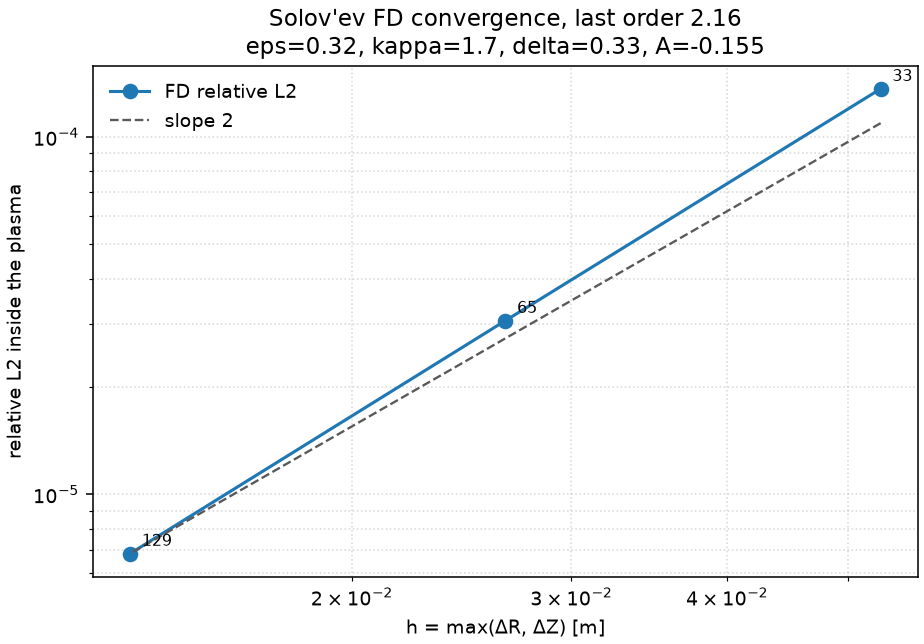
\includegraphics[width=0.72\textwidth]{solver_convergence.png}
\caption[Solver error against the analytic Solov'ev flux]{The same comparison as \cref{tab:fd}, on a log--log plot of relative \(L^{2}\) against grid spacing. The dashed reference has slope \(2\), drawn through the finest point. Point labels are the number of nodes on a side. The measured slope sits slightly above \(2\), which is the expected look of a second-order scheme on three grids with a curved boundary.}
\label{fig:conv}
\end{figure}

\section{The datasets}

Fixed-boundary samples are drawn by scrambled Sobol sequences, which fill a box in several dimensions more evenly than independent random points. The nine inputs and their in-distribution ranges (\code{data/generate.py}) are in \cref{tab:ranges}.

\begin{table}[htbp]
\centering
\caption{In-distribution ranges for the nine fixed-boundary inputs.}
\label{tab:ranges}
\small
\begin{tabular}{@{}lll@{}}
\toprule
Parameter & Range & Role \\
\midrule
\(R_{0}\) & \(\qtyrange{1.5}{1.9}{\metre}\) & geometric major radius \\
\(\varepsilon=a/R_{0}\) & \(0.25\)--\(0.40\) & inverse aspect ratio; \(a=\varepsilon R_{0}\) is stored \\
\(\kappa\) & \(1.2\)--\(2.0\) & elongation \\
\(\delta\) & \(0\)--\(0.5\) & triangularity \\
\(\Ip\) & \(\qtyrange{0.5}{2.0}{\mega\ampere}\) & plasma current \\
\(\beta_{0}\) & \(0.2\)--\(0.8\) & fraction of \(J_{\phi}\) in the pressure term \\
\(\alpha\) & \(0.8\)--\(2.5\) & current-profile exponent \\
\(\gamma\) & \(1.0\)--\(3.0\) & current-profile exponent \\
\(B_{0}\) & \(\qtyrange{1.5}{3.0}{\tesla}\) & vacuum-field scale, \(F(1)=R_{0} B_{0}\) \\
\bottomrule
\end{tabular}
\end{table}

Five thousand solves were requested and five thousand were kept: the inverse metrics record \(4000\) train, \(500\) validation, and \(500\) test. Every plasma lives on one shared grid, \(R\in[0.80,2.76]\,\mathrm{m}\), \(Z\in[-1.90,1.90]\,\mathrm{m}\), \(65\times 65\). The spacings are \(\Delta R=\qty{0.030625}{\metre}\) and \(\Delta Z=\qty{0.059375}{\metre}\). The box was chosen so that even the most elongated plasma in the out-of-distribution set sits several cells inside the boundary.

The out-of-distribution file is another \(500\) Sobol samples with the same ranges except \(\kappa\in(2.0,2.3]\), and every row is labelled test. The point of the file is extrapolation: the networks never train on elongation above \(2\), and \(2.3\) was checked to keep the level set a single closed curve and the solver convergent. The Sobol stream uses a different seed offset so the file is not a copy of the training set with \(\kappa\) edited.

The free-boundary set is FreeGS on its \code{TestTokamak} coil set (\code{P1L}, \code{P1U}, \code{P2L}, \code{P2U}), on \(R\in[0.1,2.0]\), \(Z\in[-1.0,1.0]\), again \(65\times 65\). Inputs are a poloidal beta, \(\Ip\) from \(0.1\) to \(\qty{0.4}{\mega\ampere}\), a vacuum-field parameter, two profile exponents, and X-point locations jittered around a double-null example, with about \(30\%\) of the attempts forced to a single null. A sample is kept only if the solve finishes, the current matches \(\Ip\) to \(2\%\), the core mask is sane, \(q_{95}\) lies in \((0.5,40)\), and the measured shape is physical. Of \(600\) attempts, \(298\) were kept and split \(238/30/30\). Just over half the solves were dropped. The file is a small free-boundary collection on one toy machine, which is the right way to read the FreeGS inverse numbers later.

\section*{Check your understanding}
\begin{enumerate}[label=\textbf{Q9.\arabic*.},leftmargin=2.4em]
\item \(\lambda\) is recomputed every Picard iteration. What constraint does that enforce, and what would go wrong if \(\lambda\) were left at its initial guess?
\item Why does changing \(B_{0}\) leave a fixed-boundary \(\psi\) unchanged, and which derived quantity does feel \(B_{0}\)?
\item The Shortley--Weller cut replaces the grid spacing by the true distance to the boundary. What order of error would you expect if the code had instead snapped the boundary to the nearest node?
\item The FreeGS file keeps \(298\) equilibria out of \(600\) attempts. Why should its inverse error not be lined up against the fixed-boundary inverse error as a win?
\end{enumerate}

\begin{keyideas}
\(\psi=0\) on the boundary for the solver family; \(\psibar<0\) inside for the analytic family. The current profile is a pressure piece times \(R\) plus an \(FF'\) piece times \(1/R\), shaped by \(g(\psin)\) and scaled by \(\lambda\) so the total current is \(\Ip\). Solov'ev equilibria have constant \(p'\) and \(FF'\) and an exact polynomial solution. Picard iteration with under-relaxation \(0.5\) and a Shortley--Weller boundary is second order; the \(65^{2}\) analytic error is \(3.06\times 10^{-5}\). The fixed-boundary set has \(5000\) plasmas on one grid; the OOD set pushes \(\kappa\) past \(2\); FreeGS is \(298\) kept free-boundary plasmas on one coil set.
\end{keyideas}


\chapter{Physics-informed networks}
\label{ch:pinn}

\begin{objectives}
\begin{itemize}[leftmargin=1.2em]
\item Say what a PINN is shown, and what it is not shown, during training.
\item Quote the relative \(L^{2}\) of the Solov'ev, nonlinear, and parametric cases, and compare the Solov'ev network with the finite-difference error on the same grid.
\item Explain why the nonlinear showcase is a qualitatively right equilibrium with a percent-level flux error.
\end{itemize}
\end{objectives}

A physics-informed neural network represents \(\psi(R,Z)\) by a neural network and trains the weights so that the differential equation and the boundary condition hold at collocation points, in the sense of \eqref{eq:pinn-loss}. No solved equilibrium is used as a target inside the domain. The network here is a multilayer perceptron: \(5\) hidden layers of width \(64\), hyperbolic tangent, inputs mapped affinely onto \([-1,1]\), float64 arithmetic. \(\Dstar\psi\) is built with automatic differentiation from the expanded form \eqref{eq:dstar-exp}. The loss is a normalized mean square of \(\Dstar\psi-\mathrm{rhs}\), plus a weight \(w_{b}\) times the mean square of \(\psi\) on the boundary. Boundary points are the true zero contour of the level set, found by ray bisection, so the network is pinned to the geometry rather than to a nearby Miller polyline.

Training is Adam for a few hundred steps, then L-BFGS. The budget requested in the saved runs is \(5000\) steps. L-BFGS stopped earlier: \(700\) Adam steps and \(1122\) L-BFGS closures for the Solov'ev case, \(\qty{95}{\second}\) of training (\code{outputs/pinn/solovev_metrics.json}).

Three cases were trained.

The Solov'ev case is the analytic equilibrium of \cref{ch:code}. The right-hand side is the known function of \(R\), and the reference used for scoring is \(\psibar\). On the \(129^{2}\) evaluation grid the relative \(L^{2}\) inside the plasma is \(3.15\times 10^{-4}\), the maximum pointwise error is \(2.31\times 10^{-5}\), and the largest \(\lvert\psi\rvert\) on the boundary samples is \(2.47\times 10^{-6}\). The boundary is satisfied tightly. The interior relative error is about \(46\) times the finite-difference error on the same \(129^{2}\) grid (\(3.15\times 10^{-4}\) against \(6.82\times 10^{-6}\)). The network is a useful representation of this one solution. The finite-difference solution on that grid is the more accurate of the two.

The nonlinear case is the showcase equilibrium: \(R_{0}=\qty{1.7}{\metre}\), \(a=\qty{0.6}{\metre}\), \(\kappa=1.7\), \(\delta=0.3\), \(\Ip=\qty{1}{\mega\ampere}\), \(\beta_{0}=0.5\), \(\alpha=1\), \(\gamma=2\), \(B_{0}=\qty{2}{\tesla}\). Because the right-hand side depends on \(\psi\), the training is itself a Picard loop. A constant-current warm start is followed by six lagged updates of \(\psi_{\mathrm{axis}}\) and \(\lambda\). The reference is a finite-difference solution of the same equilibrium, not an analytic formula. Relative \(L^{2}\) is \(8.48\times 10^{-3}\), the maximum pointwise error is \(4.09\times 10^{-3}\,\mathrm{Wb/rad}\), and the magnetic-axis error is \(\qty{5.03}{\milli\metre}\) (mostly in \(Z\): the reference axis is on the midplane and the network axis is \(\qty{4.49}{\milli\metre}\) low). The predicted \(\psi_{\mathrm{axis}}\) is \(0.3560\) against a reference \(0.3588\), and \(\lambda\) is off by a relative \(0.835\%\). This is a qualitatively right equilibrium with a percent-level flux error, visibly worse than the linear analytic case. One forward pass on a \(65^{2}\) grid takes \(\qty{2.05}{\milli\second}\), after \(\qty{88}{\second}\) of training that produced a network for this single plasma.

The parametric case adds \(A\) as an input, trained at five values in \([-0.3,0.1]\) and scored at four values it did not train on: \(-0.27\), \(-0.155\), \(-0.05\), and \(0.05\). The mean relative \(L^{2}\) on those four is \(1.55\times 10^{-3}\); the worst is \(1.94\times 10^{-3}\) at \(A=-0.05\). The mean magnetic-axis error over the four is \(\qty{0.338}{\milli\metre}\) (\code{outputs/compare/pinn_summary.json}). A one-parameter family of linear equilibria is well inside the reach of this small network. A nine-parameter family of nonlinear equilibria is what the surrogate in the next chapter is for.

\begin{figure}[htbp]
\centering
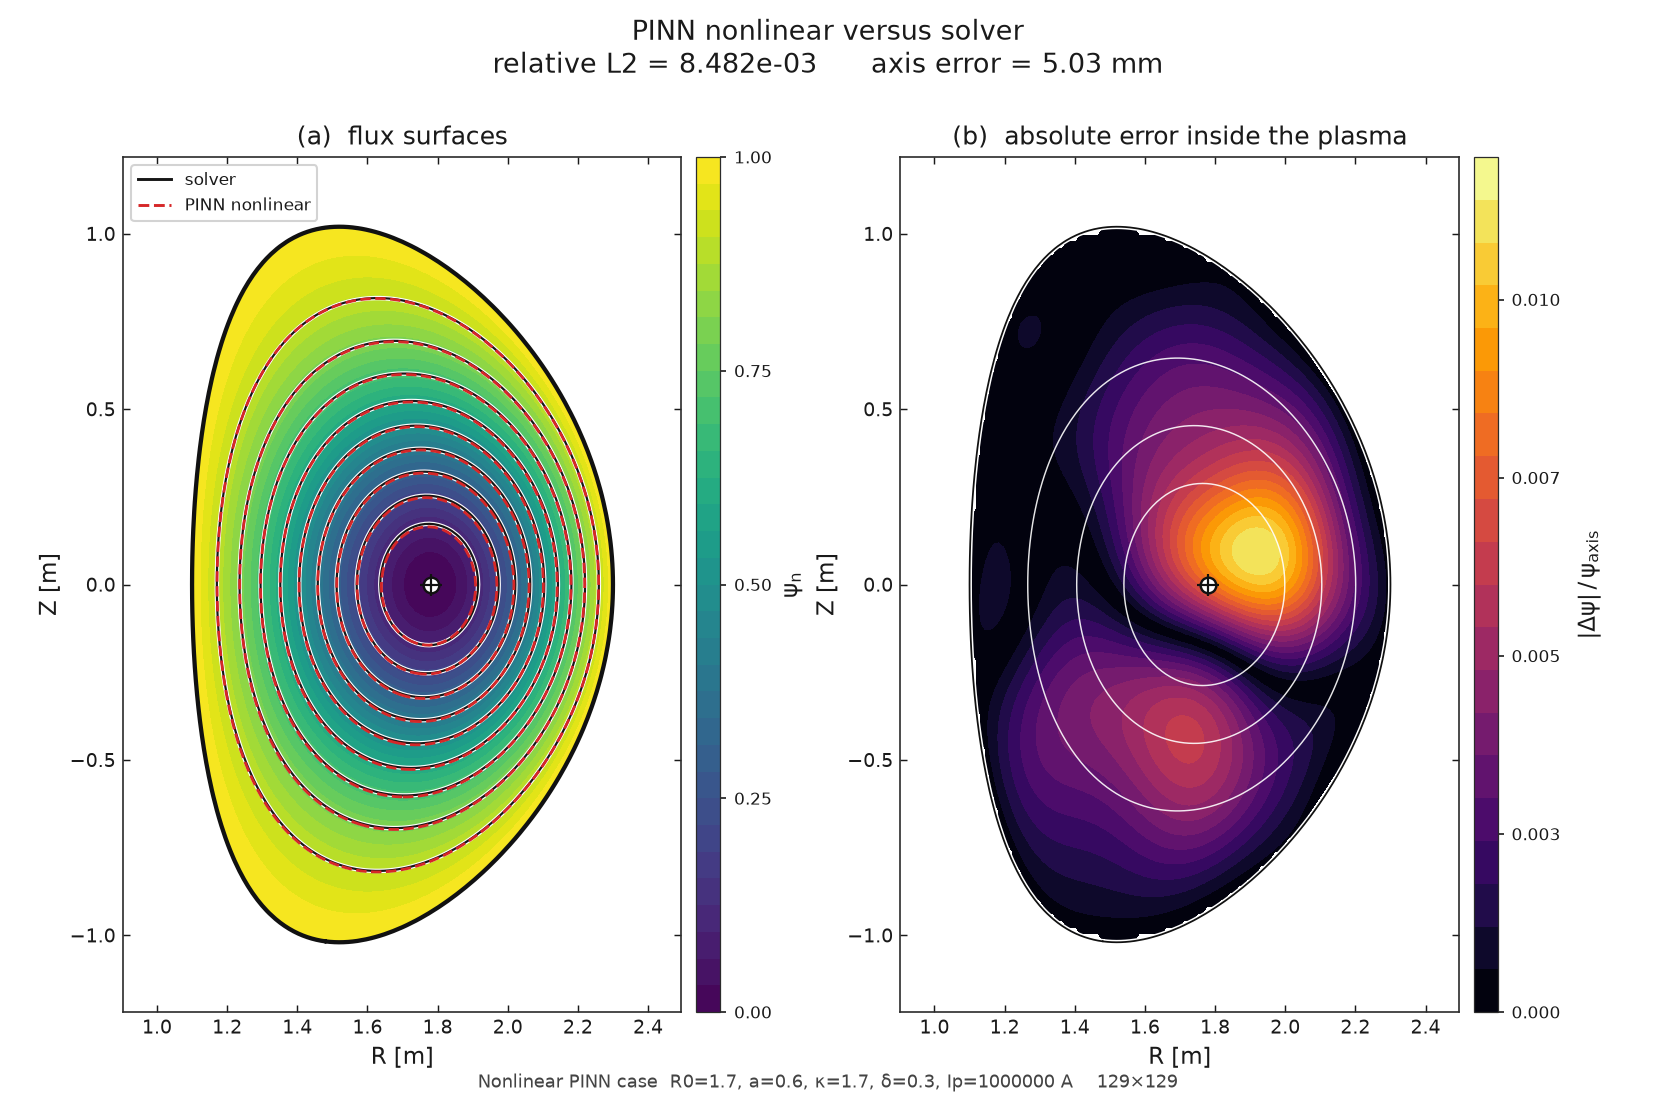
\includegraphics[width=0.96\textwidth]{pinn_vs_solver.png}
\caption[Nonlinear PINN against the solver]{Nonlinear physics-informed network on the showcase parameters, at \(129^{2}\). Solid contours are the reference solver and the network is drawn with them; the title matches the metrics file, relative \(L^{2}\) \(8.48\times 10^{-3}\) and axis error \(\qty{5.03}{\milli\metre}\). The flux surfaces agree closely. The error panel is less uniform than the surrogate's in \cref{fig:surr-one}: there is a localized patch near the axis at about one percent of \(\psi_{\mathrm{axis}}\), consistent with the \(\qty{4.5}{\milli\metre}\) vertical axis error. This network was trained on the equation for this one plasma. The surrogate was trained on four thousand plasmas and happens to be a bit worse on this particular flux norm and better on the axis.}
\label{fig:pinn-one}
\end{figure}

\begin{figure}[p]
\centering
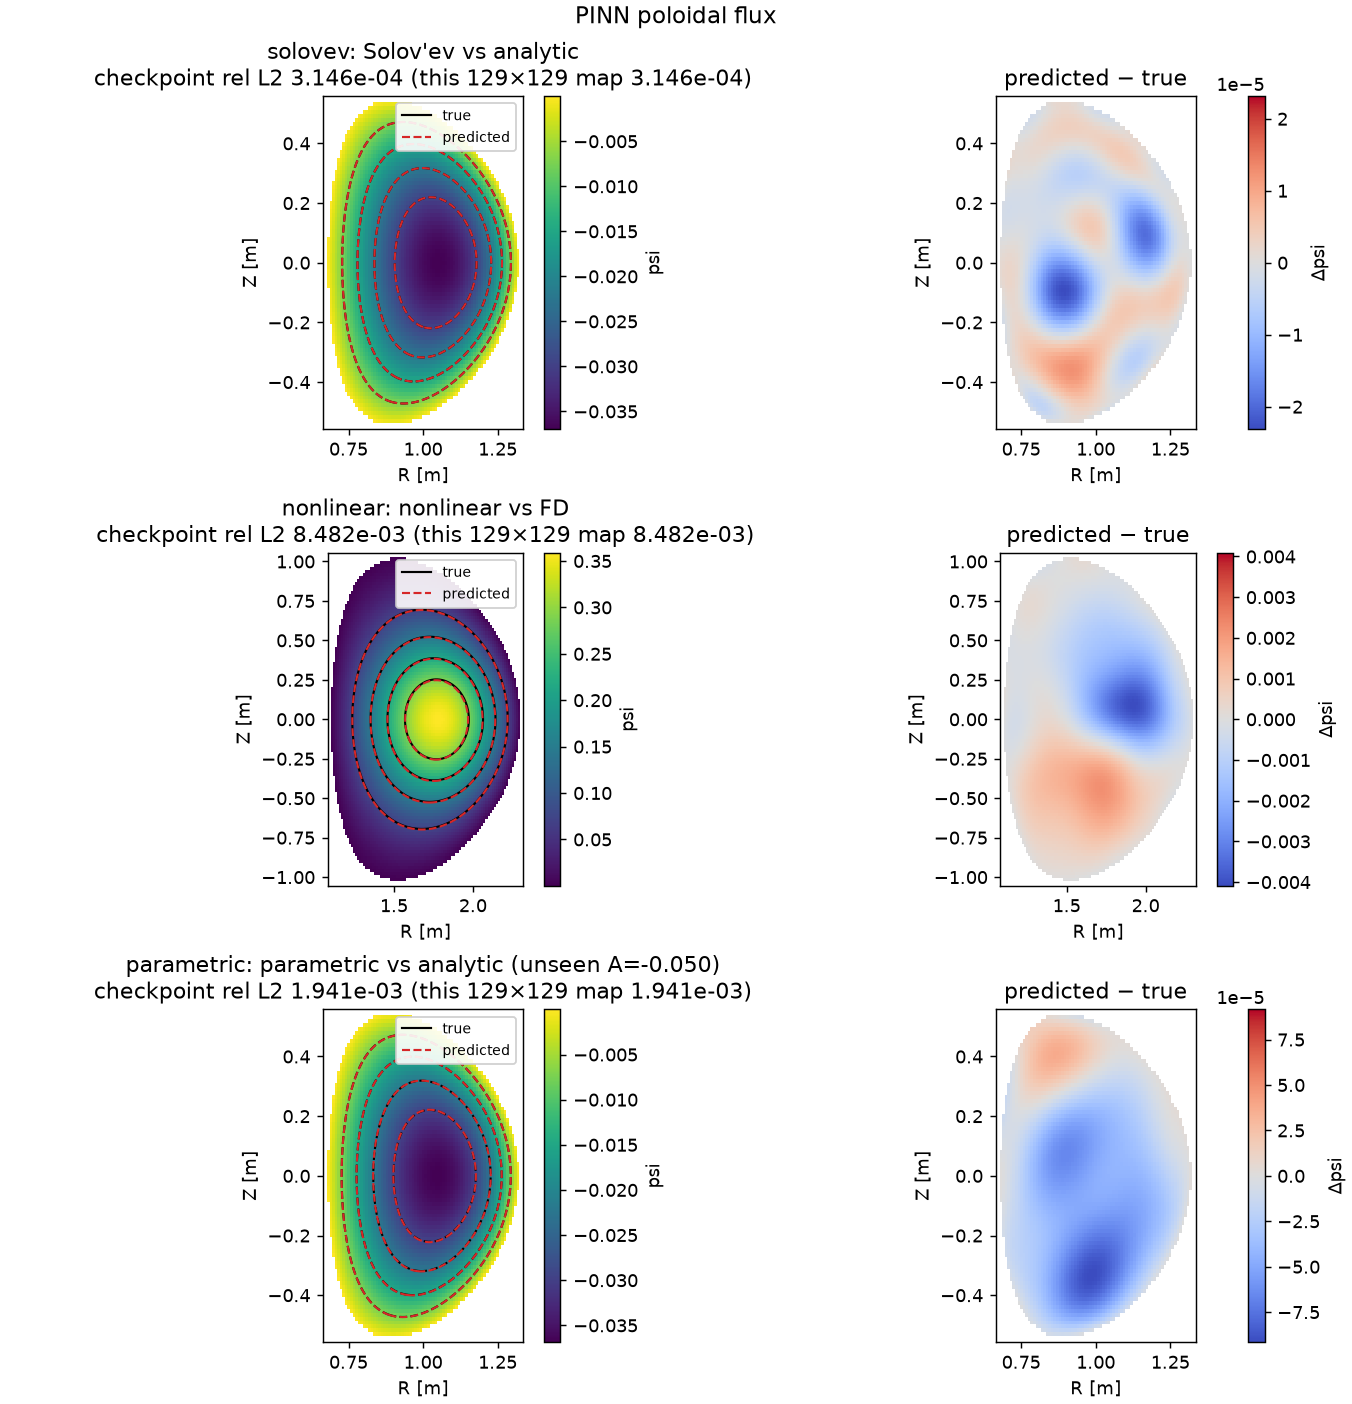
\includegraphics[width=0.82\textwidth]{pinn_comparison.png}
\caption[The three physics-informed cases]{The three physics-informed cases. Each row is the reference flux with the network contour over it, and the pointwise error. Solov'ev and nonlinear use the full reference. The parametric row is the worst unseen value, \(A=-0.05\), whose relative \(L^{2}\) is \(1.94\times 10^{-3}\). The axis error printed on that single panel is not the \(\qty{0.338}{\milli\metre}\) mean over all four unseen values; the mean is the number in the summary table.}
\label{fig:pinn-all}
\end{figure}

\section*{Check your understanding}
\begin{enumerate}[label=\textbf{Q10.\arabic*.},leftmargin=2.6em]
\item The Solov'ev PINN has relative \(L^{2}\) \(3.15\times 10^{-4}\) on the \(129^{2}\) grid. The finite-difference error on that grid is \(6.82\times 10^{-6}\). Which representation is more accurate, and by about what factor?
\item Why is the nonlinear training a Picard loop, while the Solov'ev training is not?
\item The parametric network is scored at \(A=-0.05\). Was that value in the training set?
\end{enumerate}

\begin{keyideas}
The PINN is fit to the residual of \(\Dstar\psi\) and to \(\psi=0\) on the true boundary. It is not shown an interior solution. On the linear Solov'ev problem it reaches \(3.15\times 10^{-4}\), about \(46\) times the finite-difference error on the same grid. On the nonlinear showcase it reaches \(8.48\times 10^{-3}\) and an axis error of \(\qty{5.03}{\milli\metre}\). A one-parameter linear family is learned to about \(1.55\times 10^{-3}\) mean relative \(L^{2}\) on four unseen values of \(A\). The network is a useful representation of one solution. On a grid this size the finite-difference solve is the more accurate of the two.
\end{keyideas}

\chapter{Learning the forward map}
\label{ch:surrogate}

\begin{objectives}
\begin{itemize}[leftmargin=1.2em]
\item Describe the two surrogate architectures and why \(\psi\) is predicted as a shape times a scale.
\item Read the four-run table: what the physics weight changes, and what it barely changes.
\item Explain the checkerboard-versus-bump experiment, and what the OOD elongation scan says about generalization.
\end{itemize}
\end{objectives}

The surrogate is an ordinary regression from the nine parameters to the \(65\times 65\) field \(\psi\), trained on the \(4000\) solved equilibria. Two architectures are in \code{models/surrogate.py}.

The MLP--CNN encodes the nine numbers with a small fully connected network, reshapes them into an \(8\times 8\) feature image, and decodes with three stride-2 transposed convolutions up to \(64\times 64\), then a bilinear resize to \(65\times 65\). A final convolution also sees the normalized coordinates \((R,Z)\) and the parameters broadcast over the grid. That last step matters: a plain convolutional stack is translation-equivariant, and a tokamak is not. The plasma sits at a particular \(R\). This model has \(629002\) parameters.

The Fourier neural operator lifts a field of channels --- the parameters broadcast in space, the coordinates, and the plasma mask --- into a width-\(16\) representation, applies three Fourier layers that keep \(8\) modes, and projects back to one channel. It has \(202786\) parameters. It is handed the mask, so it is told the boundary geometry directly. The comparison below is between these two specific sizes, trained for \(36\) epochs (MLP--CNN) or \(24\) epochs (FNO). It is not a general verdict on the two families.

Both models predict a shape and a scale separately. A head predicts \(\log\psi_{\mathrm{axis}}\), the spatial network predicts the dimensionless field \(\psi/\psi_{\mathrm{axis}}\), and the physical flux is the product. On this dataset \(\psi_{\mathrm{axis}}\) varies by about an order of magnitude because \(\Ip\) and the plasma size vary, while the shape inside the mask stays in \([0,1]\). Dividing by the per-sample axis value stops the loss from being dominated by the high-current plasmas. An extra mean-square penalty on \(\log\psi_{\mathrm{axis}}\) stops the shape and the scale from trading off against each other.

The optional physics term is
\begin{equation}
\label{eq:wphys}
w_{\mathrm{phys}}\,
\frac{\lVert\Dstar\psi_{\mathrm{pred}}+\mu_{0} R J_{\mathrm{true}}\rVert^{2}}
{\lVert\mu_{0} R J_{\mathrm{true}}\rVert^{2}},
\end{equation}
evaluated on nodes whose four neighbours are also inside the plasma, with the same conservative stencil as the solver. \(w_{\mathrm{phys}}\) is \(0\) for the first few epochs and then \(0.1\). The denominator makes the weight dimensionless. The true current is used, so this term asks the predicted flux to be consistent with the current of the equilibrium it is copying. It is not a free-standing solver.

Mean errors on the \(500\) test equilibria, and on the \(500\) high-elongation equilibria, from \code{outputs/surrogate/summary.json}, are in \cref{tab:surr}.

\begin{table}[htbp]
\centering
\caption{Surrogate means. \(q_{95}\) uses the true \(F(\psin)\) and the predicted geometry, on \(50\) test equilibria. The relative error is \(\lvert q_{\mathrm{pred}}-q_{\mathrm{true}}\rvert/\lvert q_{\mathrm{true}}\rvert\) at \(\psin=0.95\). An LCFS failure means the contour \(\psi=10^{-3}\psi_{\mathrm{axis}}\) could not be drawn around the axis.}
\label{tab:surr}
\footnotesize
\setlength{\tabcolsep}{4.2pt}
\begin{tabular}{@{}lcccccc@{}}
\toprule
Run & test rel \(L^{2}\) & OOD rel \(L^{2}\) & GS residual & axis & \(q_{95}\) rel & LCFS fail \\
\midrule
MLP--CNN, \(w=0\) & \(1.42\times 10^{-2}\) & \(2.15\times 10^{-2}\) & \(0.977\) & \(\qty{8.36}{\milli\metre}\) & \(0.136\) & \(55/500\) \\
MLP--CNN, \(w=0.1\) & \(1.09\times 10^{-2}\) & \(1.86\times 10^{-2}\) & \(0.0327\) & \(\qty{1.40}{\milli\metre}\) & \(0.0243\) & \(0/500\) \\
FNO, \(w=0\) & \(2.46\times 10^{-2}\) & \(3.89\times 10^{-2}\) & \(0.564\) & \(\qty{5.77}{\milli\metre}\) & \(0.260\) & \(132/500\) \\
FNO, \(w=0.1\) & \(2.11\times 10^{-2}\) & \(3.64\times 10^{-2}\) & \(0.0510\) & \(\qty{3.39}{\milli\metre}\) & \(0.274\) & \(82/500\) \\
\bottomrule
\end{tabular}
\end{table}

LCFS error is the symmetric mean distance between those contours. The mean LCFS distance for the best model is \(\qty{13.0}{\milli\metre}\) on all \(500\) test plasmas. For the MLP--CNN without the physics term the mean is \(\qty{36.2}{\milli\metre}\), and it is computed only on the \(445\) contours that succeeded, so it is an optimistic summary of a model that also fails outright on \(55\) plasmas.

Read the MLP--CNN pair first. Relative \(L^{2}\) only moves from \(1.42\%\) to \(1.09\%\). The Grad--Shafranov residual drops by a factor of thirty, from \(0.977\) to \(0.0327\). The axis error drops from \(\qty{8.4}{\milli\metre}\) to \(\qty{1.4}{\milli\metre}\), and the relative \(q_{95}\) error from \(14\%\) to \(2.4\%\). The same pattern, weaker, is there in the FNO residual and the FNO axis. The FNO \(q_{95}\) error does not improve (\(0.260\) to \(0.274\)). A physics penalty is not automatically helpful for every derived quantity on every architecture.

The residual can move so much while \(L^{2}\) barely moves because \(\Dstar\) is a second-derivative operator. A small, rapid wiggle in \(\psi\) costs little in an \(L^{2}\) norm and a great deal once two derivatives hit it. \(q\) and the axis location are sensitive to the same derivatives: \(B_{p}\) is \(\lvert\grad\psi\rvert/R\), and the axis is a critical point of \(\psi\). An \(L^{2}\)-only fit is free to leave high-frequency error that those quantities notice.

This is easy to see on a single solved equilibrium. Take the showcase plasma on the \(129^{2}\) nonlinear-PINN box, \(R\in[0.90,2.55]\,\mathrm{m}\) and \(Z\in[-1.25,1.25]\,\mathrm{m}\), add a perturbation whose relative \(L^{2}\) against \(\psi\) is exactly \(0.01\), and recompute \code{eval.metrics.gs_residual} against the unchanged \(-\mu_{0} R J\). A smooth Gaussian bump of width \(\qty{0.35}{\metre}\) produces a normalized residual of \(8.84\times 10^{-3}\). A grid-scale checkerboard, \(\sin(\pi R/\Delta R)\sin(\pi Z/\Delta Z)\) masked to the plasma, produces a residual of \(23.3\). The same \(1\%\) of flux error changes the residual by a factor of \(2.64\times 10^{3}\) when it is oscillatory. The unperturbed solver residual on that equilibrium is \(1.5\times 10^{-8}\), so the discrete solution does satisfy the discrete equation. The physics loss is a way of telling the network that the second kind of error is unacceptable even when the flux plot looks fine.

Out of distribution, at \(\kappa\in(2.0,2.3]\), the best model goes from \(1.09\times 10^{-2}\) to \(1.86\times 10^{-2}\) in relative \(L^{2}\) and from \(\qty{1.40}{\milli\metre}\) to \(\qty{2.30}{\milli\metre}\) in axis error. The degradation is real and it is not a collapse. Without the physics term the OOD axis error is \(\qty{22.4}{\milli\metre}\), and \(86\) of \(500\) LCFS contours fail. The FNO out of distribution fails the LCFS contour on \(372\) of \(500\) plasmas even with the physics term. Elongation past the training range is mostly a shape-generalization test, and the coordinate-aware CNN with the residual penalty is the one that keeps the surfaces usable.

On speed, \code{outputs/compare/speed.json} is the comparison to use, and \cref{fig:speed} is that file. One \(65\times 65\) nonlinear solve of the showcase equilibrium takes \(\qty{44.32}{\milli\second}\). One sample through \code{mlpcnn_pw0p1} takes \(\qty{1.05}{\milli\second}\). A batch of the \(500\) test plasmas takes \(\qty{273.42}{\milli\second}\). The training-time logs inside each surrogate metrics file quote a different single-solve time, about \(\qty{27}{\milli\second}\), because that timer wrapped a different call. Both are ``tens of milliseconds.'' Neither makes the finite-difference solver look slow. The batch throughput is where the surrogate is actually cheaper, and only after the \(\qty{241}{\second}\) of training for that checkpoint.

\begin{figure}[htbp]
\centering
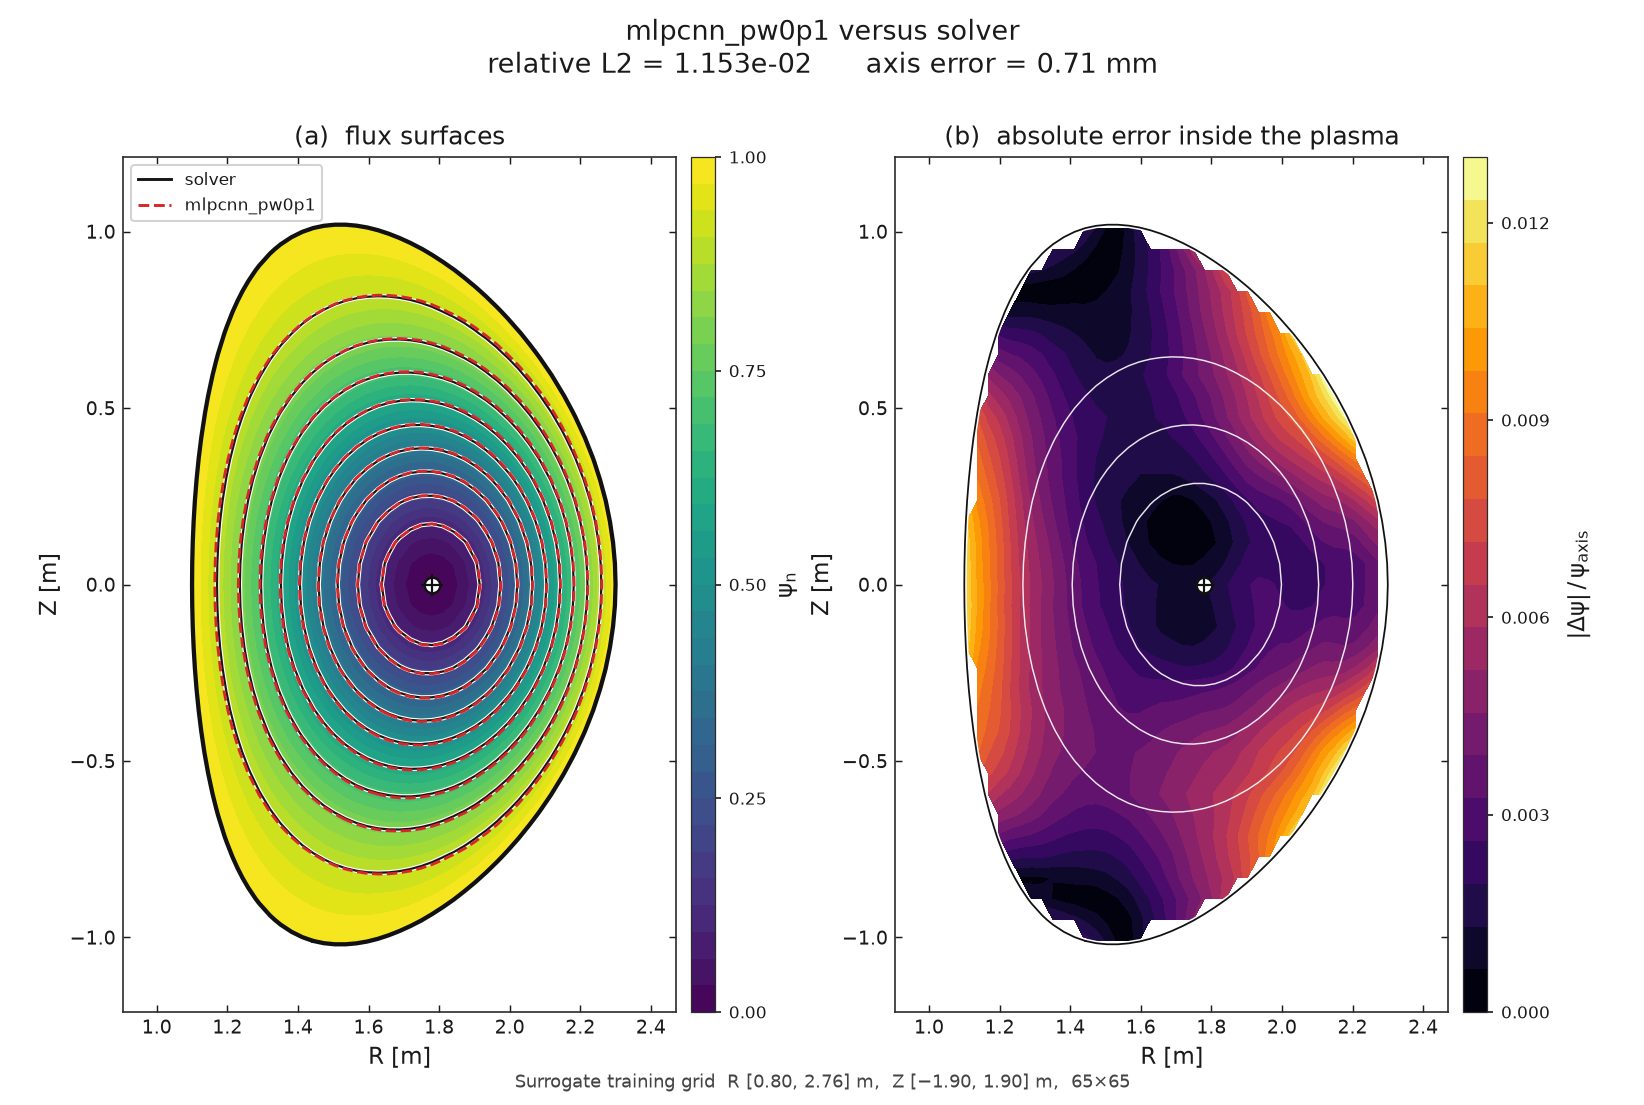
\includegraphics[width=0.96\textwidth]{surrogate_vs_solver.png}
\caption[Best surrogate on the showcase equilibrium]{\code{mlpcnn_pw0p1} on the showcase equilibrium, on the \(65\times 65\) training grid. Solid contours are the solver and dashed contours are the network. The title reports relative \(L^{2}\) \(1.153\times 10^{-2}\) and an axis error of \(\qty{0.71}{\milli\metre}\) for this particular plasma. Those are one sample, not the test-set means (\(1.09\times 10^{-2}\) and \(\qty{1.40}{\milli\metre}\)). A single plasma can land on either side of the mean. Panel~(b) is \(\lvert\Delta\psi\rvert/\psi_{\mathrm{axis}}\) inside the LCFS. The error is a few parts in a thousand over most of the core and larger toward the edge, where the colour scale reaches about \(0.013\). The surfaces in panel~(a) still lie on top of each other at the width of the line.}
\label{fig:surr-one}
\end{figure}

\begin{figure}[p]
\centering
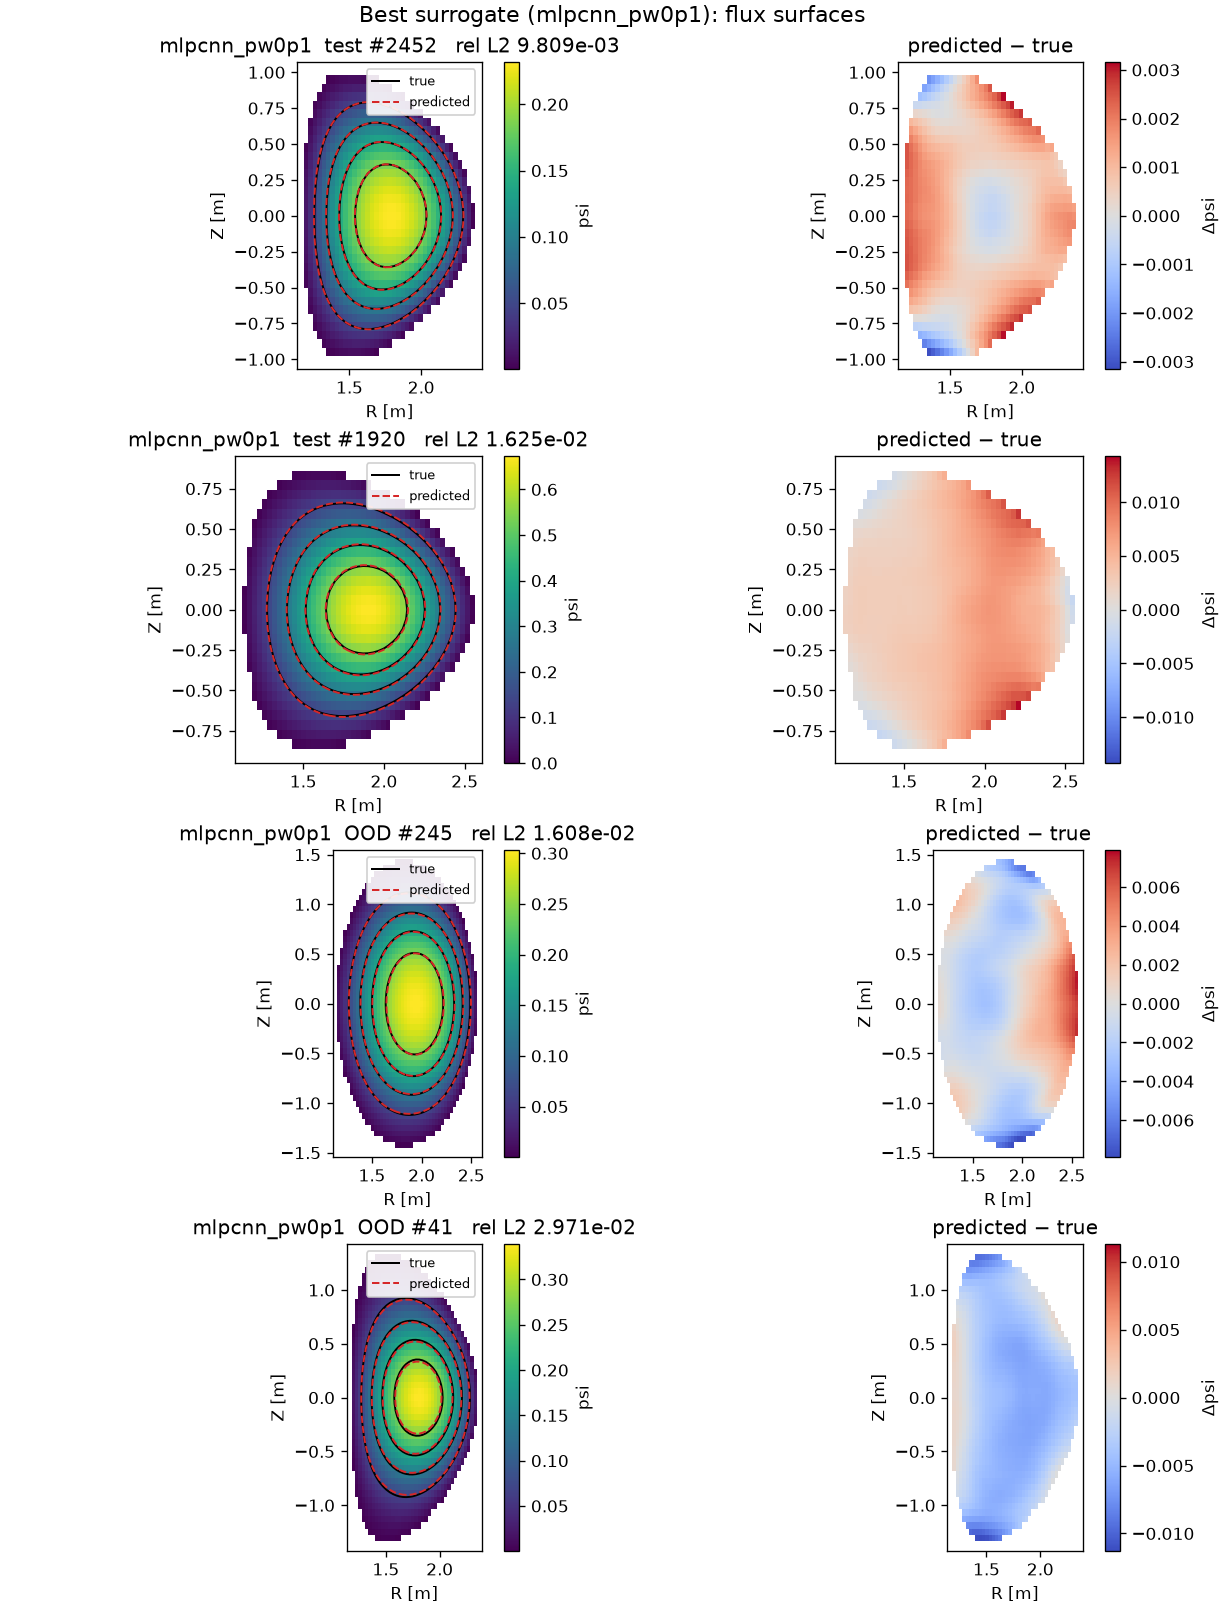
\includegraphics[width=0.78\textwidth]{surrogate_samples.png}
\caption[Surrogate at the median and the 90th percentile]{Best surrogate on four plasmas chosen by flux error: the median and the 90th percentile of the test split, then the same two quantiles of the high-elongation set. The panels are test \(\#2452\) at \(9.81\times 10^{-3}\), test \(\#1920\) at \(1.63\times 10^{-2}\), OOD \(\#245\) at \(1.61\times 10^{-2}\), and OOD \(\#41\) at \(2.97\times 10^{-2}\). Black contours are the solver and dashed contours are the network. The right column is the signed error \(\psi_{\mathrm{pred}}-\psi_{\mathrm{true}}\). Even the worst of these four still has the right topology: one axis, nested surfaces, the boundary in the right place. The error changes sign across the plasma rather than being a pure scale mistake, which is what the separate \(\psi_{\mathrm{axis}}\) head was meant to prevent.}
\label{fig:surr-samples}
\end{figure}

\begin{figure}[htbp]
\centering
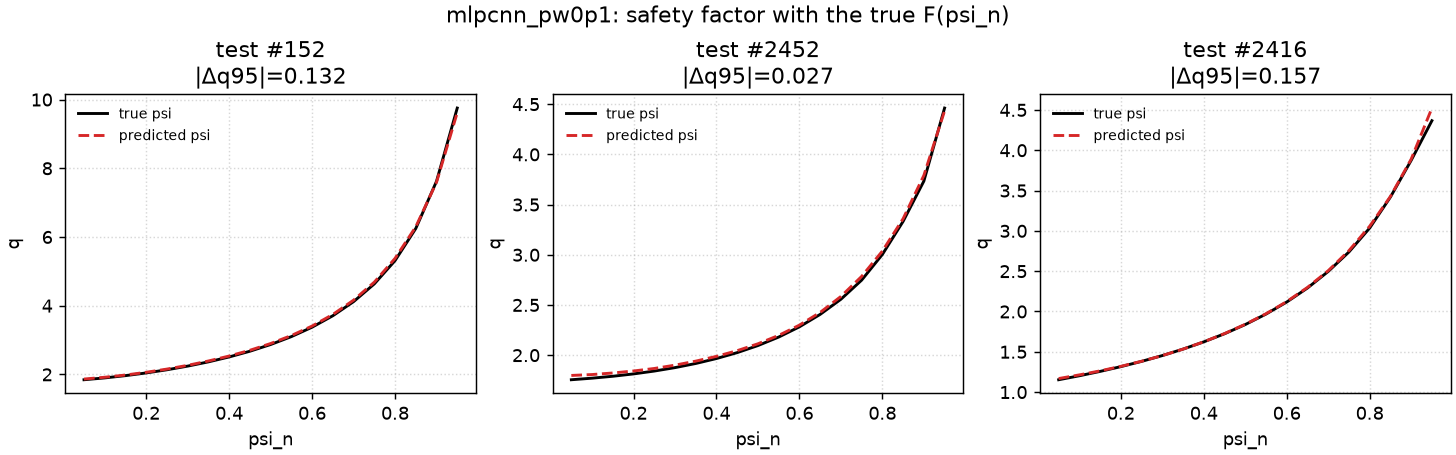
\includegraphics[width=\textwidth]{surrogate_q.png}
\caption[Safety factor on three test plasmas]{\(q(\psin)\) for three test plasmas of \code{mlpcnn_pw0p1}, using the true \(F\). The panels are test \(\#152\), \(\#2452\), and \(\#2416\), with absolute \(q_{95}\) errors \(0.132\), \(0.027\), and \(0.157\). The curves overlie each other. These three were chosen as quartiles of the flux error, and their \(q_{95}\) errors happen to sit around the test-set mean absolute error of \(0.087\). The plot is evidence that a one-percent flux error, for this model, moves \(q\) by a few hundredths, provided \(F\) is known exactly. It is not evidence about an error in \(F\).}
\label{fig:surr-q}
\end{figure}

\begin{figure}[p]
\centering
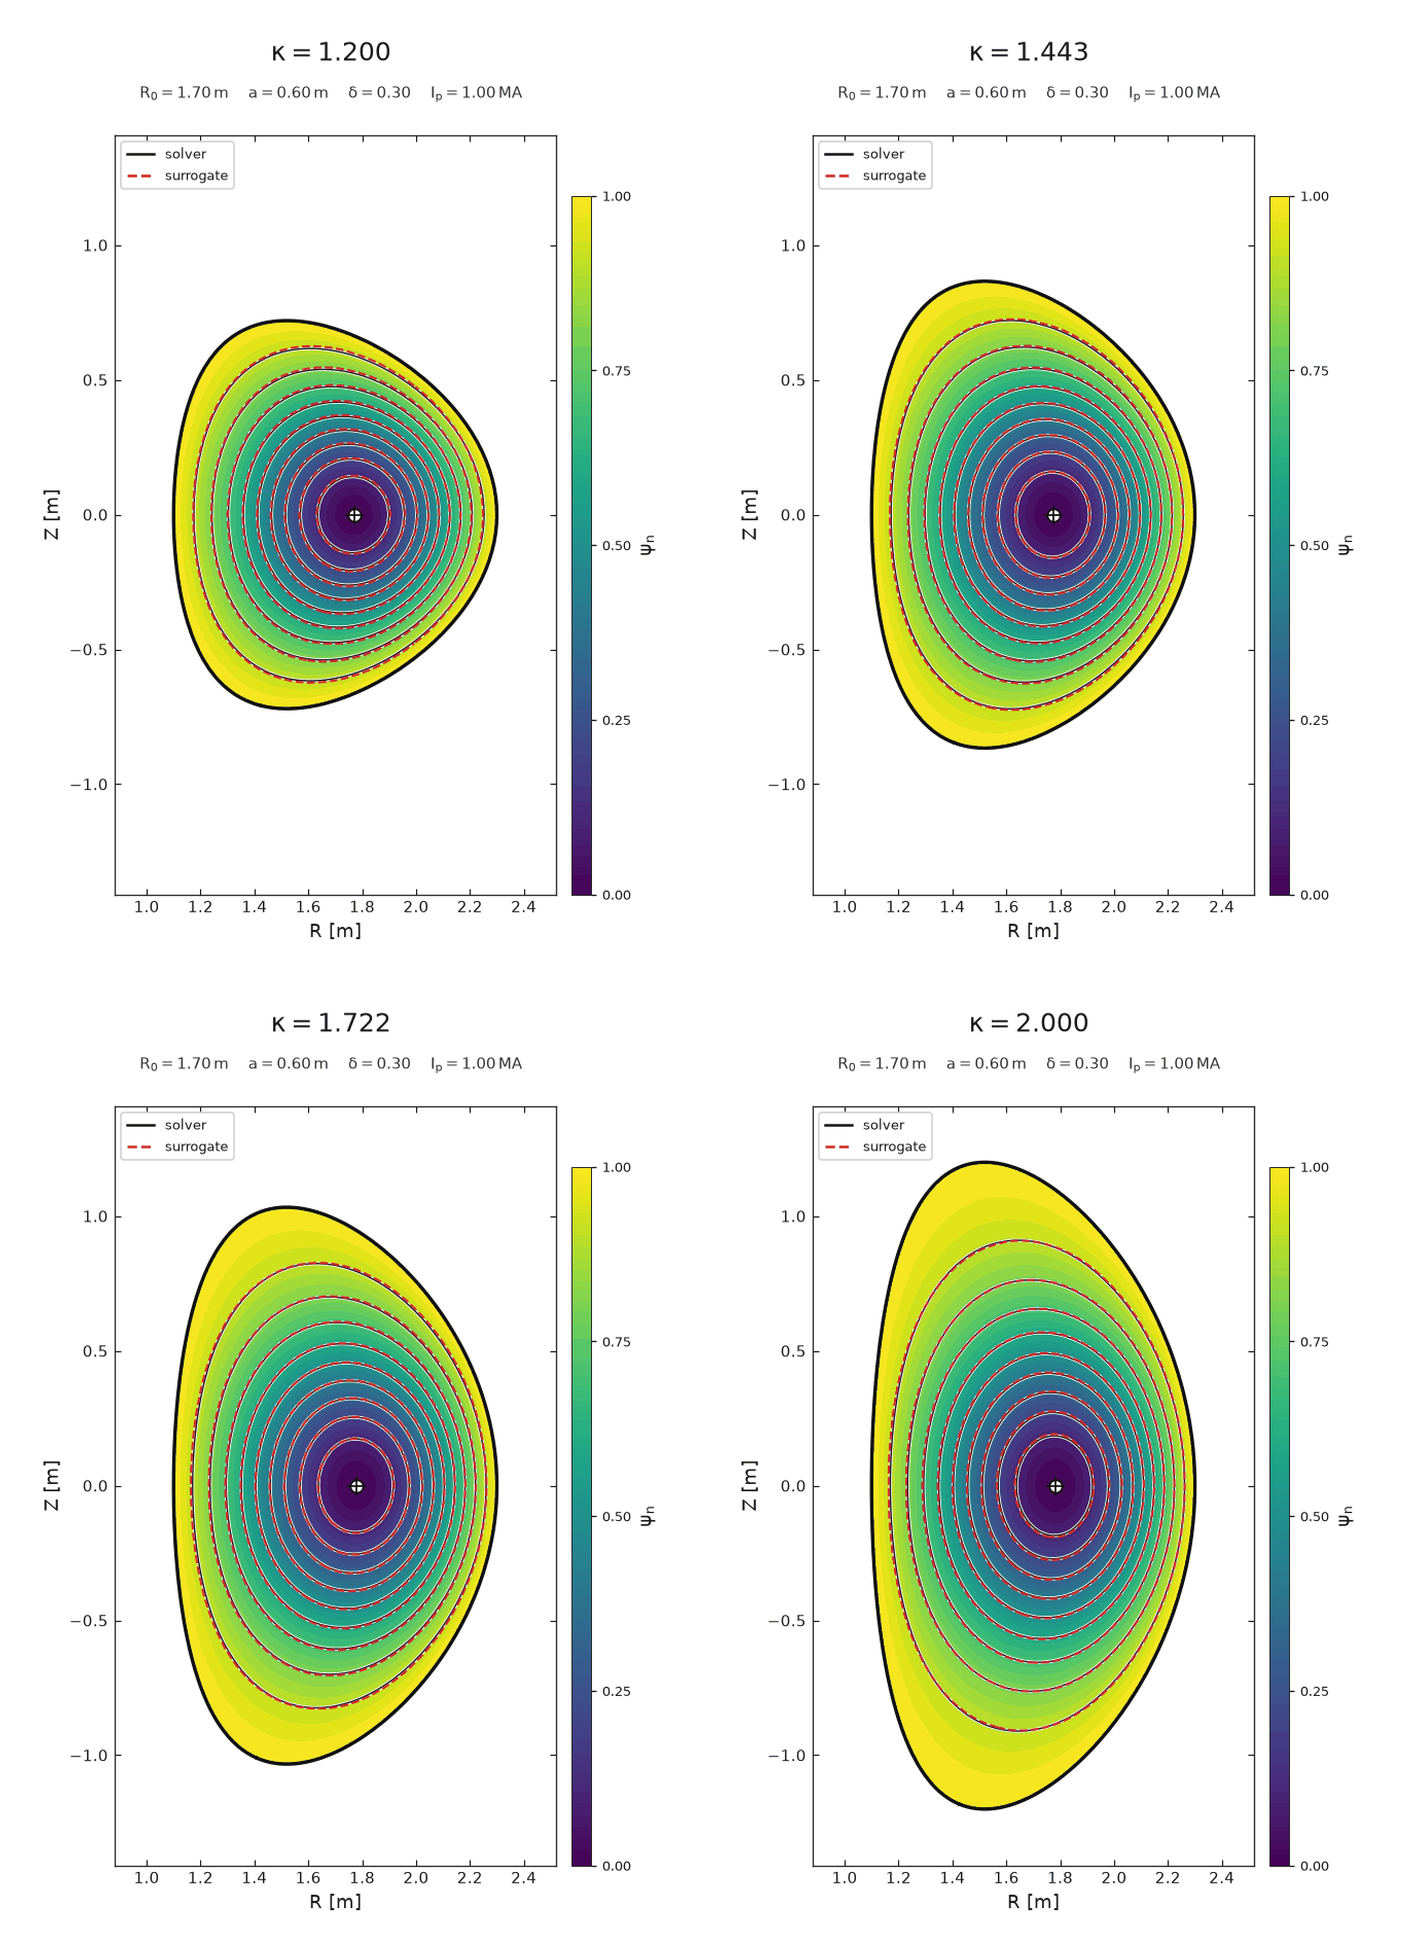
\includegraphics[width=0.90\textwidth]{kappa_sweep_frames.png}
\caption[Four frames of the elongation sweep]{Four frames of the showcase equilibrium with \(\kappa\) running from \(1.2\) to \(2.0\) and every other parameter fixed. Solid contours are the solver and dashed contours are the surrogate. The axes are held fixed, so the plasma is seen to grow taller; through the training range the dashed curves track the solid ones. The animated file in the repository, \code{docs/figures/kappa_sweep.gif}, has all \(24\) frames. The out-of-distribution test, \(\kappa\) up to \(2.3\), is the numerical version of pushing that animation past its last frame; the numbers are in \cref{tab:surr}. The triangularity animation was left out of the figures folder to keep the size down. It is the same script with \(\delta\) from \(0\) to \(0.5\).}
\label{fig:kappa}
\end{figure}

\section*{Check your understanding}
\begin{enumerate}[label=\textbf{Q11.\arabic*.},leftmargin=2.6em]
\item Relative \(L^{2}\) for the MLP--CNN moves from \(1.42\times 10^{-2}\) to \(1.09\times 10^{-2}\) when the physics weight is turned on. Which three scores move much more, and which FNO score does not improve?
\item A \(1\%\) Gaussian bump and a \(1\%\) checkerboard produce residuals \(8.84\times 10^{-3}\) and \(23.3\). Why does the physics loss care about the difference?
\item The FNO is handed the plasma mask and has fewer parameters. Why is the table still not a verdict that MLPs beat Fourier operators?
\end{enumerate}

\begin{keyideas}
The surrogate maps nine parameters to \(\psi\). Predicting \(\log\psi_{\mathrm{axis}}\) and a dimensionless shape stops the loss from being dominated by high-current plasmas. A Grad--Shafranov penalty of weight \(0.1\), using the true current, barely changes relative \(L^{2}\) and drops the residual, the axis error, and \(q_{95}\) error on the MLP--CNN. The same \(1\%\) of flux error can be harmless or disastrous once two derivatives hit it. Outside the training range in \(\kappa\) the best model degrades from \(1.09\times 10^{-2}\) to \(1.86\times 10^{-2}\) and keeps a usable boundary. The batch, not the single solve, is where it is cheaper than Picard iteration.
\end{keyideas}

\chapter{Reconstruction from external magnetics}
\label{ch:inverse}

\begin{objectives}
\begin{itemize}[leftmargin=1.2em]
\item List the \(101\) synthetic channels and the noise model.
\item Use the \(R^{2}\) table to say which parameters external magnetics determine.
\item Explain what the hybrid experiment adds: the error floor is missing information, not a weak forward model.
\end{itemize}
\end{objectives}

Reconstruction runs the map backwards. The sensors are a synthetic diagnostic set, \code{SensorSet} in \code{models/diagnostics.py}, sitting on a closed vessel. For the fixed-boundary data the vessel is a D-shaped contour inset just inside the grid box, outside every plasma in the training file and in the elongation file. The channels, \(101\) of them, are:
\begin{itemize}[leftmargin=1.2em]
\item \(40\) pickup coils measuring the tangential poloidal field \(B_{t}=\mathbf{B}\cdot\hat{\mathbf{t}}\),
\item \(40\) pickup coils measuring the outward normal field \(B_{n}=\mathbf{B}\cdot\hat{\mathbf{n}}\),
\item \(20\) flux loops measuring \(\psi\) at points on the vessel,
\item one Rogowski coil, which is the vessel contour itself and returns the total toroidal current inside it.
\end{itemize}

The response of a sensor to the plasma is a Green's function. A unit toroidal filament at \((R_{c},Z_{c})\) produces poloidal flux per radian
\begin{equation}
\label{eq:green}
\psi=\frac{\mu_{0}}{2\pi}\sqrt{R R_{c}}\,
\frac{(2-k^{2})K(k^{2})-2E(k^{2})}{k},
\end{equation}
\begin{equation}
\label{eq:k2}
k^{2}=\frac{4 R R_{c}}{(R+R_{c})^{2}+(Z-Z_{c})^{2}},
\end{equation}
with \(K\) and \(E\) the complete elliptic integrals. \(B_{R}\) and \(B_{Z}\) are central differences of this flux with a step of \(10^{-3}\,\mathrm{m}\), the same step FreeGS uses. The code comments that this step is a few parts in \(10^{5}\) relative to the analytic derivative, well below the \(1\%\) sensor noise. The full response matrix \(G\) has one column per grid cell. Signals are \(G\) times the cell currents \(J\,\Delta R\,\Delta Z\). Because the stored fixed-boundary flux is zero outside the plasma, these sensors see the plasma current only. There are no poloidal-field coils in the fixed-boundary sensor model. The Rogowski row of \(G\) is \(1\) on cells inside the vessel and \(0\) outside, so its signal is \(\Ip\).

Noise is independent Gaussian noise on each channel with standard deviation equal to \code{noise} times that channel's root-mean-square over the training set. The saved model used \(\mathrm{noise}=0.01\). Inputs to the network include the raw signals, the same signals divided by the Rogowski channel, and the log of the Rogowski signal, so the current amplitude and the shape of the magnetic pattern are separate features. Poloidal-field coil currents are appended for the FreeGS model.

The selected architecture is the direct one (\code{outputs/inverse/metrics.json}, \(48\) epochs, \(\qty{508}{\second}\)). An MLP encodes the diagnostics to a latent vector. A convolutional decoder, the same skeleton as the surrogate, predicts the shape \(\psi/\psi_{\mathrm{axis}}\), and a scalar head predicts \(\log\psi_{\mathrm{axis}}\). A second head predicts the equilibrium parameters. That head is what the \(R^{2}\) numbers below are measuring. It is not the path that produces \(\psi\) in the direct model. The loss includes the flux error, the parameter error, and a small Grad--Shafranov penalty of weight \(0.05\) against the true current.

On the fixed-boundary test split the relative \(L^{2}\) of \(\psi\) is \(0.1707\) (median \(0.151\)). The validation and training relative \(L^{2}\) values are \(0.1751\) and \(0.1688\). The network is not overfitting. The magnetic-axis error is \(\qty{6.06}{\milli\metre}\), the LCFS distance is \(\qty{65.6}{\milli\metre}\) on the \(454\) contours that succeeded (\(46\) failed), the Grad--Shafranov residual is \(0.205\), and the absolute \(q_{95}\) error is \(1.403\) on \(50\) equilibria. That \(q_{95}\) comparison, like the surrogate one, uses the true \(F\) built from the true parameters. The error is entirely from the geometry of the predicted \(\psi\). An absolute error of \(1.4\) on a quantity that is typically a few units is a different statement from the surrogate's \(2.4\%\) relative error. Out of distribution the flux error is \(0.1894\) and the absolute \(q_{95}\) error is \(1.436\).

The noise sweep is the first clue that this floor is not the noise. \Cref{tab:noise} is the sweep.

\begin{table}[htbp]
\centering
\caption{Inverse relative \(L^{2}\) against the relative noise on each channel.}
\label{tab:noise}
\small
\begin{tabular}{@{}lccc@{}}
\toprule
Relative noise & in-distribution rel \(L^{2}\) & OOD rel \(L^{2}\) & FreeGS rel \(L^{2}\) \\
\midrule
\(0\) & \(0.1704\) & \(0.1882\) & \(0.1142\) \\
\(0.01\) & \(0.1707\) & \(0.1894\) & \(0.1154\) \\
\(0.03\) & \(0.1777\) & \(0.1953\) & \(0.1192\) \\
\(0.05\) & \(0.1887\) & \(0.2040\) & \(0.1244\) \\
\bottomrule
\end{tabular}
\end{table}

From clean signals to \(1\%\) noise the test error moves in the fourth digit. At \(5\%\) noise it has risen from \(0.170\) to \(0.189\). The reconstruction was already \(17\%\) wrong with perfect measurements.

The parameter \(R^{2}\) on clean signals (\code{param_r2_clean} in the same file) says what is wrong. \Cref{tab:r2} is that list, together with the values at \(1\%\) noise.

\begin{table}[htbp]
\centering
\caption{Coefficient of determination for the inverse parameter head. \(R^{2}=0\) is no better than guessing the training mean.}
\label{tab:r2}
\small
\begin{tabular}{@{}lcc@{}}
\toprule
Parameter & clean \(R^{2}\) & \(R^{2}\) at \(1\%\) noise \\
\midrule
\(\Ip\) & \(0.999\) & \(0.999\) \\
\(R_{0}\) & \(0.961\) & \(0.960\) \\
\(\delta\) & \(0.578\) & \(0.488\) \\
\(\kappa\) & \(0.515\) & \(0.494\) \\
\(a\) & \(0.434\) & \(0.429\) \\
\(\gamma\) & \(0.407\) & \(0.391\) \\
\(\alpha\) & \(0.219\) & \(0.218\) \\
\(\beta_{0}\) & \(0.002\) & \(0.000\) \\
\(B_{0}\) & \(-0.026\) & \(-0.026\) \\
\bottomrule
\end{tabular}
\end{table}

\(R^{2}=1\) would mean the parameter is recovered perfectly. \(R^{2}=0\) means the prediction is no better than guessing the training mean. A slightly negative value means it is a little worse than that.

\(\Ip\) is essentially perfect because the Rogowski coil measures it. \(R_{0}\) is well determined because the external field pattern knows where the current sits. The boundary parameters are only partly visible: the vessel is well outside the plasma, and more than one shape can produce a similar external field. \(\alpha\) and \(\gamma\), which set the radial shape of the current, are weakly determined. \(\beta_{0}\) is not determined at all.

That last fact is the classical one. External magnetics respond to the poloidal field outside the plasma. By Amp\`ere's law they fix the total current. They also fix, for a circular plasma, the combination \(\beta_{p}+l_{i}/2\), because a broader current (lower internal inductance) and a higher poloidal beta can be arranged to leave the same field at the wall. Shaping separates the two only weakly, which is why EFIT with magnetics alone is not trusted for the current profile (Lao et al., 1985). In this parameterization \(\beta_{0}\) is the knob that trades pressure against the \(FF'\) part of the current, and \(\alpha\), \(\gamma\) move the peaking. The \(R^{2}\) values are that degeneracy, restricted to the profile family the network was shown. \(B_{0}\) has \(R^{2}\approx 0\) for a simpler reason: it never enters \(\psi\), and none of these sensors measure \(B_{\phi}\).

The hybrid experiment closes the argument. A second network maps the sensors to the nine parameters and then through the frozen \code{mlpcnn_pw0p1} surrogate, which itself has test relative \(L^{2}\) \(0.0109\) when it is given the true parameters. The hybrid's test relative \(L^{2}\) is \(0.1696\). The direct decoder's is \(0.1707\). Feeding a much more accurate forward model does not move the flux error. The floor is the part of the equilibrium the sensors do not determine. A production reconstruction adds internal constraints that this sensor set leaves out: motional Stark effect measurements of the local field-line pitch, which constrain \(q\) and hence the current profile, and Thomson scattering or other kinetic measurements of the pressure.

The FreeGS inverse is a different and smaller experiment. It trains on \(238\) equilibria, tests on \(30\), and is given the four poloidal-field coil currents as well as the magnetic signals. Test relative \(L^{2}\) is \(0.1154\), the axis error is \(\qty{12.1}{\milli\metre}\), and the LCFS distance is \(\qty{17.3}{\milli\metre}\) on \(28\) of \(30\) contours. The \(q_{95}\) score is empty, \(30\) failures out of \(30\), because the scoring routine builds \(F(\psi)\) from the fixed-boundary parameter names and a FreeGS row does not have them. That is a missing metric, not thirty plasmas with no safety factor. The lower flux error should not be lined up against \(0.171\) as a win. The coil currents are known inputs, the machine is one fixed coil set, and the test set has \(30\) rows. One \code{reconstruct} call takes \(\qty{1.20}{\milli\second}\) for either checkpoint.

\begin{figure}[htbp]
\centering
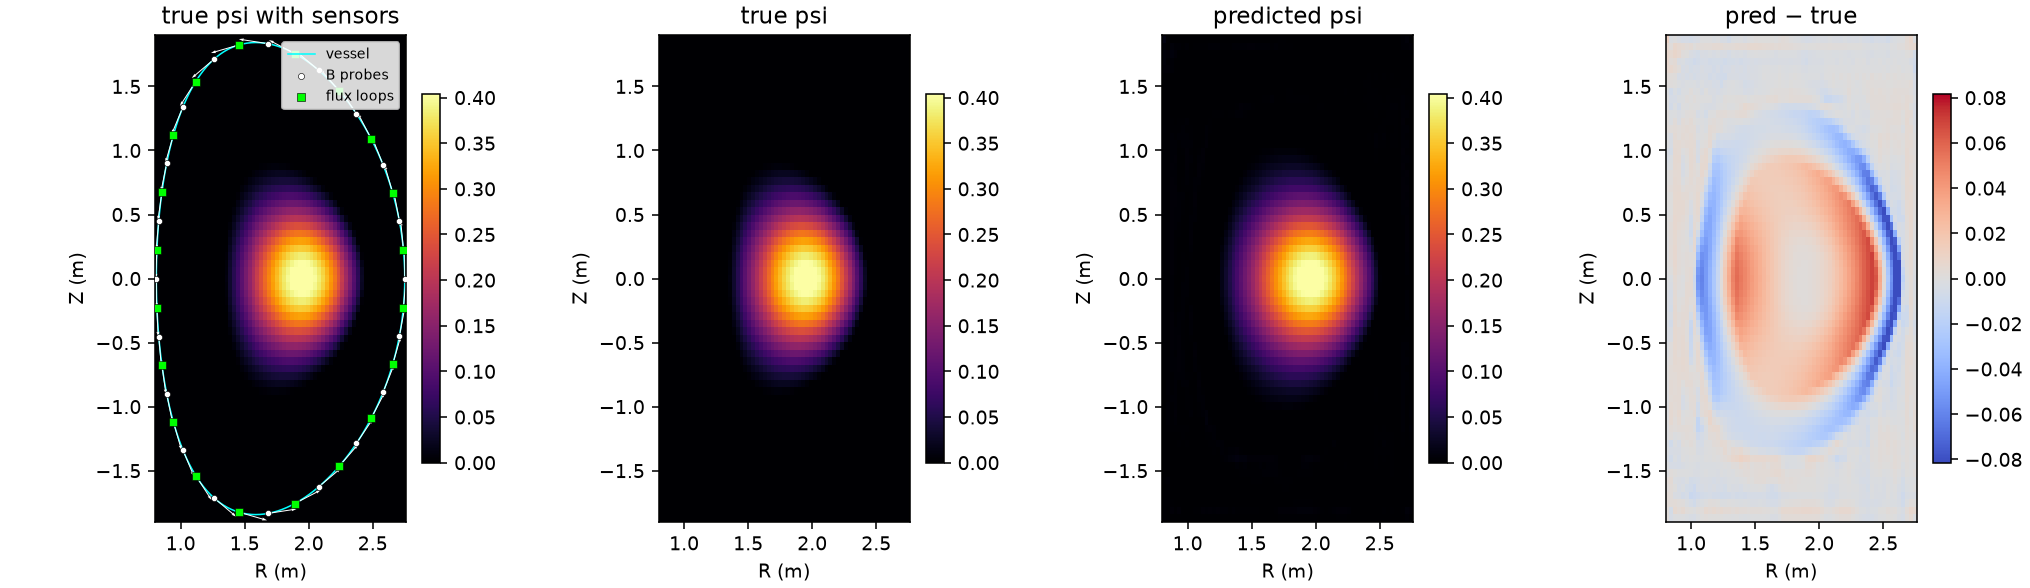
\includegraphics[width=\textwidth]{inverse_reconstruction.png}
\caption[Inverse reconstruction of one fixed-boundary plasma]{One fixed-boundary reconstruction. The first panel is the true \(\psi\) with the vessel, the pickup coils, and the flux loops. The second is the true flux, the third is the network, and the fourth is the difference. The predicted plasma is in the right place and has the right sign, and the error map is a smooth redistribution at several hundredths of a \(\mathrm{Wb/rad}\), on a flux whose axis value is a few tenths. That is the visual form of a \(0.17\) relative \(L^{2}\): the gross current and position are there, and the internal distribution is not.}
\label{fig:inv}
\end{figure}

\begin{figure}[htbp]
\centering
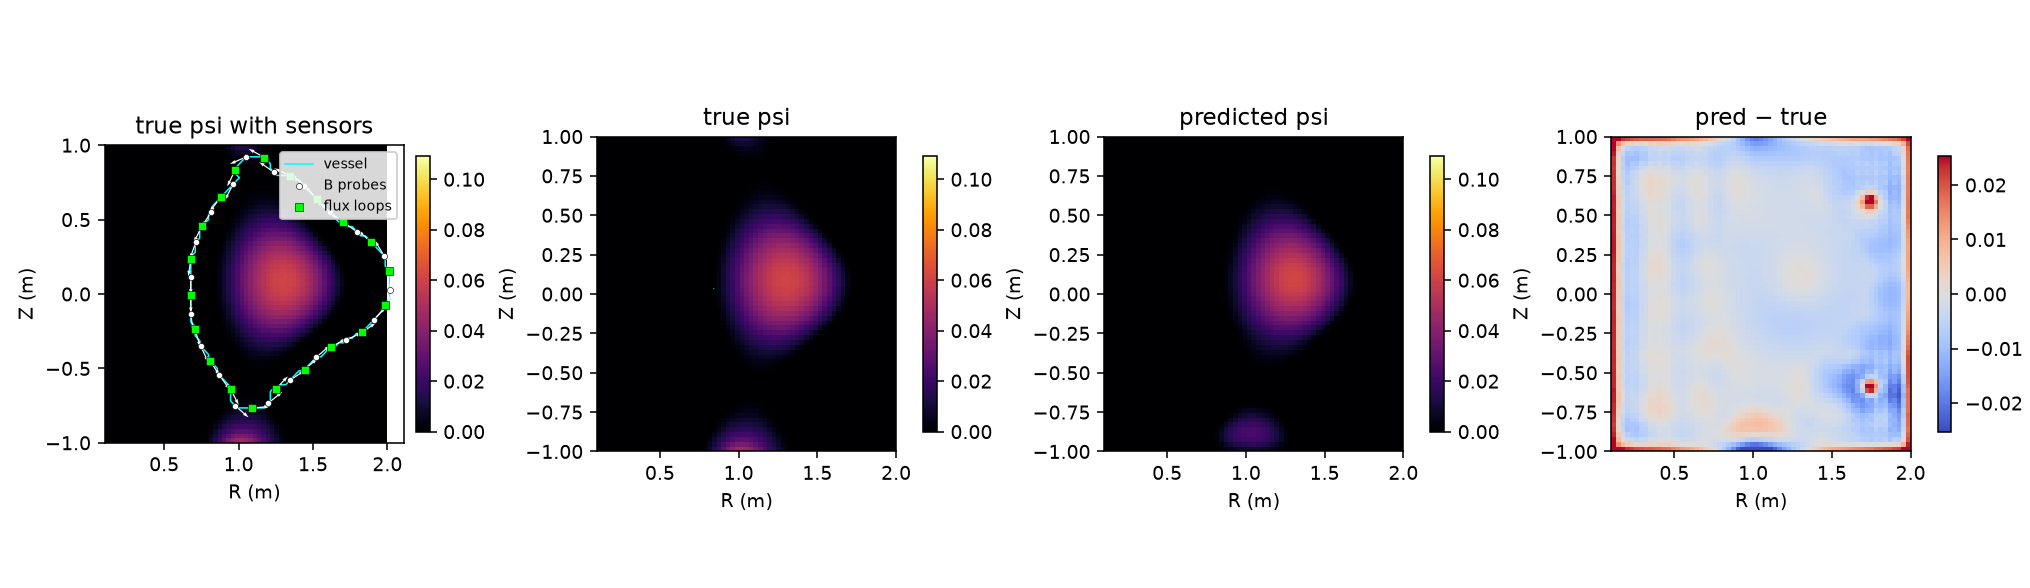
\includegraphics[width=\textwidth]{inverse_freegs_reconstruction.png}
\caption[FreeGS inverse reconstruction]{The same four panels for one free-boundary sample. The vessel is the TestTokamak wall, and the network was also given the four poloidal-field coil currents. Do not read the lower flux error on this set as a better inverse model: thirty plasmas, one coil set, coil currents handed to the network.}
\label{fig:inv-fg}
\end{figure}

\begin{figure}[htbp]
\centering
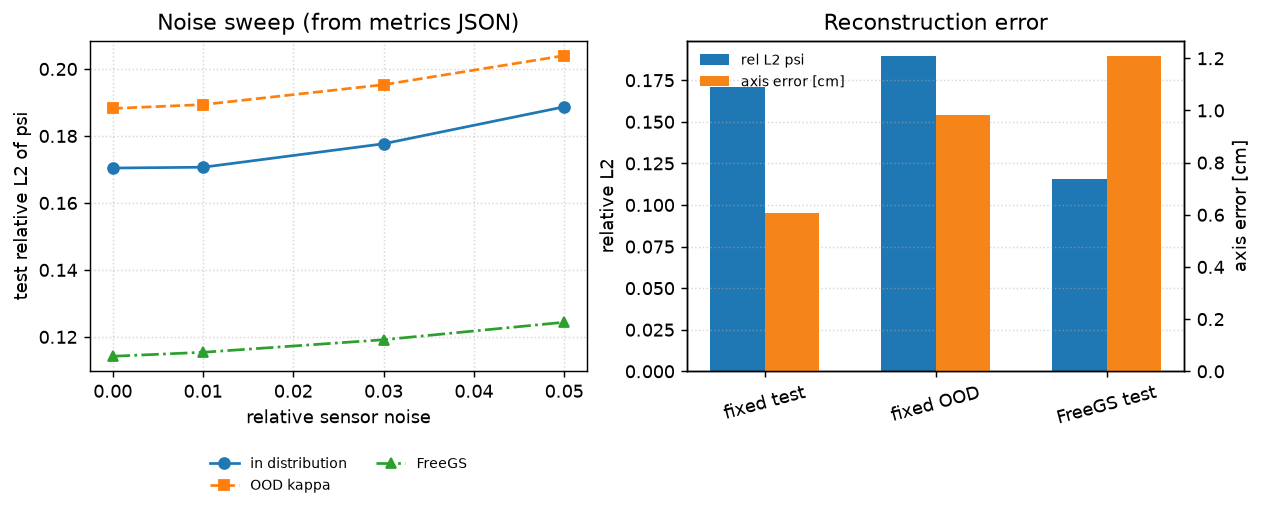
\includegraphics[width=0.96\textwidth]{inverse_summary.png}
\caption[Inverse noise sweep and axis error]{The noise table and the headline errors. The left panel is almost flat between \(0\) and \(1\%\) noise for all three datasets, then bends up. The right panel compares relative \(L^{2}\) (left axis) with axis error in centimetres (right axis). Fixed-boundary test and OOD have the larger flux error and the smaller axis error. The FreeGS test has a smaller flux error and an axis error of about \(\qty{1.2}{\centi\metre}\). Axis error and flux error are not substitutes for each other.}
\label{fig:inv-sum}
\end{figure}

\section*{Check your understanding}
\begin{enumerate}[label=\textbf{Q12.\arabic*.},leftmargin=2.6em]
\item \(\Ip\) has \(R^{2}=0.999\) and \(\beta_{0}\) has \(R^{2}=0.002\) on clean signals. Which sensor, or which missing measurement, is responsible for each?
\item The hybrid model routes the sensors through a surrogate whose relative \(L^{2}\) is \(0.0109\) when the parameters are true, and still scores \(0.1696\). What does that equality with the direct model (\(0.1707\)) rule out?
\item Why is \(B_{0}\) unpredictable from this diagnostic set even before noise is added?
\end{enumerate}

\begin{keyideas}
External magnetics fix \(\Ip\) (the Rogowski coil) and \(R_{0}\) (where the current sits). They do not fix \(\beta_{0}\), and they only weakly fix \(\alpha\) and \(\gamma\). That is the Shafranov--Lao degeneracy between \(\beta_{p}\) and \(l_{i}\), seen here as \(R^{2}\) values. The flux error is \(0.171\) already at zero noise, and a hybrid that uses an accurate forward surrogate does not beat it. The FreeGS inverse, at \(0.115\), is a smaller experiment with coil currents provided. The next measurement that would move the floor is an internal one.
\end{keyideas}

\chapter{A reader's guide to the figures}
\label{ch:figures}

\begin{objectives}
\begin{itemize}[leftmargin=1.2em]
\item Point to the figure that answers a given question: geometry, profiles, discretization, forward error, or inverse error.
\item Distinguish a one-plasma picture from a test-set mean.
\item Say where the animated elongation scan lives, and what pushing it past the last frame corresponds to.
\end{itemize}
\end{objectives}

The figures are placed next to the argument they illustrate. This chapter is the index, and it records a few comparisons that are easy to miss when each picture is read alone. The two diagrams drawn for the source note, rather than copied from \code{outputs/}, are \cref{fig:cross,fig:profiles}. Both were made by \code{docs/figures/make_diagrams.py} with the project's solver. The cross-section solves the showcase equilibrium on the shared fixed-boundary box at \(129\times 129\) and overlays \code{SensorSet.for_grid}. The profile figure solves the same shape at \(\beta_{0}=0.2\), \(0.5\), and \(0.8\) on a \(97^{2}\) grid in the box \(R\in[0.90,2.55]\), \(Z\in[-1.25,1.25]\), and draws Miller curves from \eqref{eq:miller}.

\Cref{fig:equilibrium} is the default case of \code{eval.visualize}. The numbers in its caption are that solve, not the test-set means of any learned model. \Cref{fig:conv} is \cref{tab:fd} drawn on log--log axes. \Cref{fig:speed} is the timing file, not a training curve.

When a learned model is drawn on one plasma, read the title as that plasma. \Cref{fig:surr-one} reports relative \(L^{2}\) \(1.153\times 10^{-2}\) and an axis error of \(\qty{0.71}{\milli\metre}\). The test-set means for the same checkpoint are \(1.09\times 10^{-2}\) and \(\qty{1.40}{\milli\metre}\). One sample sits on either side of the mean as a matter of course. \Cref{fig:pinn-one} is the nonlinear PINN on the same parameters, at a finer grid, and it is a different experiment: one plasma, trained from the equation, not from four thousand solutions.

\Cref{fig:pinn-all} stacks the three PINN cases. The parametric row is the worst unseen \(A\), not the mean over the four. \Cref{fig:surr-samples} is four quantiles of the flux error, two in distribution and two out. Topology survives on all four: one axis, nested surfaces, the boundary in the right place. \Cref{fig:surr-q} uses the true \(F\). Agreement of those \(q\) curves is evidence about the geometry of \(\psi\), not about an error in \(F\). The three plasmas were chosen as quartiles of the flux error; their absolute \(q_{95}\) errors \(0.132\), \(0.027\), and \(0.157\) happen to sit around the test-set mean absolute error of \(0.087\).

\Cref{fig:kappa} shows four frames. The repository file \code{docs/figures/kappa_sweep.gif} is the \(24\)-frame animation, with \(\kappa\) from \(1.2\) to \(2.0\). The OOD numbers, \(\kappa\) up to \(2.3\), are what you would see by continuing past the last frame. The triangularity sweep is the same script and is not in the folder.

\Cref{fig:inv,fig:inv-fg,fig:inv-sum} are the inverse story in pictures. A smooth error of several hundredths of a \(\mathrm{Wb/rad}\), on an axis value of a few tenths, is what \(0.17\) relative \(L^{2}\) looks like. The summary figure's two vertical axes are a warning: the FreeGS point has the smaller flux error and the larger axis error. Those are not two words for the same success.

\section*{Check your understanding}
\begin{enumerate}[label=\textbf{Q13.\arabic*.},leftmargin=2.6em]
\item \Cref{fig:surr-one} quotes an axis error of \(\qty{0.71}{\milli\metre}\). The table quotes \(\qty{1.40}{\milli\metre}\). Which number would you use to describe the checkpoint?
\item \Cref{fig:surr-q} shows \(q(\psin)\) for three plasmas with the curves nearly on top of each other. What was held fixed in \(F\), and what does the plot therefore not say?
\item Where is the animated elongation scan, and which saved test corresponds to running it past \(\kappa=2\)?
\end{enumerate}

\begin{keyideas}
Geometry and sensors are \cref{fig:cross}. Profiles and the Miller target are \cref{fig:profiles}. The showcase solve, with its bookkeeping, is \cref{fig:equilibrium}. One-plasma titles are not test-set means. Quantile galleries test topology, not a single lucky equilibrium. The GIF in \code{docs/figures/} is the full \(\kappa\) sweep; the OOD file is that sweep continued past the training range. Inverse flux error and inverse axis error answer different questions.
\end{keyideas}

\chapter{What the numbers mean}
\label{ch:means}

\begin{objectives}
\begin{itemize}[leftmargin=1.2em]
\item Place \(3\times 10^{-5}\), \(10^{-2}\), and \(0.17\) on one scale of claims.
\item Name the two comparisons the tables invite and do not support.
\item Say what a percent-level \(q_{95}\) error is enough for, and what it is starting to matter for.
\end{itemize}
\end{objectives}

\Cref{tab:headline} is \code{outputs/compare/summary.md}, with the same rounding that file uses. Relative \(L^{2}\) for the learned models is inside the plasma. Surrogate \(q_{95}\) errors are relative. The inverse \(q_{95}\) error is absolute, because that is what its metrics file stores. Times are the medians from \code{speed.json}.

\begin{table}[htbp]
\centering
\caption{Headline comparison. OOD numbers, where the source file prints them, are in parentheses. The inverse \(q_{95}\) error is absolute; surrogate \(q_{95}\) errors are relative.}
\label{tab:headline}
\footnotesize
\setlength{\tabcolsep}{3.6pt}
\begin{tabularx}{\textwidth}{@{}>{\raggedright\arraybackslash}p{2.55cm} >{\raggedright\arraybackslash}Y c c c c@{}}
\toprule
Model & What it is asked & rel \(L^{2}\) of \(\psi\) & axis & \(q_{95}\) & time \\
\midrule
FD, Solov'ev, \(65^{2}\) & match the analytic flux & \(3.06\times 10^{-5}\) & --- & --- & --- \\
FD, nonlinear, \(65^{2}\) & the reference solve & reference & --- & --- & \(\qty{44.3}{\milli\second}\) \\
PINN, Solov'ev & one linear equilibrium & \(3.15\times 10^{-4}\) & \(\qty{0.047}{\milli\metre}\) & --- & \(\qty{2.06}{\milli\second}\) \\
PINN, nonlinear & one nonlinear equilibrium & \(8.48\times 10^{-3}\) & \(\qty{5.03}{\milli\metre}\) & --- & \(\qty{2.05}{\milli\second}\) \\
PINN, parametric & four unseen \(A\) & \(1.55\times 10^{-3}\) mean & \(\qty{0.338}{\milli\metre}\) & --- & \(\qty{2.07}{\milli\second}\) \\
MLP--CNN, no physics & parameters to \(\psi\) & \(1.42\times 10^{-2}\) {\scriptsize(OOD \(2.15\times 10^{-2}\))} & \(\qty{8.36}{\milli\metre}\) & \(0.136\) rel & \(\qty{1.09}{\milli\second}\) \\
MLP--CNN, physics \(0.1\) & parameters to \(\psi\) & \(1.09\times 10^{-2}\) {\scriptsize(OOD \(1.86\times 10^{-2}\))} & \(\qty{1.40}{\milli\metre}\) & \(0.0243\) rel & \(\qty{1.05}{\milli\second}\) \\
FNO, no physics & parameters to \(\psi\) & \(2.46\times 10^{-2}\) {\scriptsize(OOD \(3.89\times 10^{-2}\))} & \(\qty{5.77}{\milli\metre}\) & \(0.260\) rel & \(\qty{2.89}{\milli\second}\) \\
FNO, physics \(0.1\) & parameters to \(\psi\) & \(2.11\times 10^{-2}\) {\scriptsize(OOD \(3.64\times 10^{-2}\))} & \(\qty{3.39}{\milli\metre}\) & \(0.274\) rel & \(\qty{2.84}{\milli\second}\) \\
Inverse, fixed boundary & \(101\) sensors, \(1\%\) noise & \(0.171\) {\scriptsize(OOD \(0.189\))} & \(\qty{6.06}{\milli\metre}\) & \(1.40\) abs & \(\qty{1.20}{\milli\second}\) \\
Inverse, FreeGS & sensors plus coil currents & \(0.115\) & \(\qty{12.1}{\milli\metre}\) & --- & \(\qty{1.20}{\milli\second}\) \\
\bottomrule
\end{tabularx}
\end{table}

A relative \(L^{2}\) of \(3\times 10^{-5}\) is the solver agreeing with an exact solution. It is the right standard for the discretization, and it is a much tighter standard than any of the learned models reach.

A relative \(L^{2}\) near \(10^{-2}\), with the physics penalty, keeps the magnetic axis to a millimetre or two and \(q_{95}\) to a few percent when \(F\) is known. For drawing flux surfaces, for a coarse parameter scan, or for a warm start, that is enough. For a stability calculation that cares whether \(q=1\) or \(q=2\) sits at a particular radius, a few percent on \(q_{95}\) is starting to matter, and the absolute \(q_{95}\) error of the inverse model is already past that line.

A relative \(L^{2}\) of \(0.17\) from external magnetics is a successful demonstration of a limit. The network found \(\Ip\) and \(R_{0}\), placed the axis to \(\qty{6}{\milli\metre}\), and could not see \(\beta_{0}\). Training longer, or routing the prediction through a better surrogate, does not create the missing measurement. The useful next instrument is an internal one.

Two traps are worth naming because the tables invite them. The FreeGS inverse's \(0.115\) is not a better inverse model in general; it is thirty plasmas on one coil set with the coil currents handed to the network. The solver's \(\qty{44}{\milli\second}\) is not a slow equilibrium code; it is a fixed-boundary Picard iteration on a modest grid, and the networks are fast relative to that specific baseline.

\section*{Check your understanding}
\begin{enumerate}[label=\textbf{Q14.\arabic*.},leftmargin=2.6em]
\item Put these three relative \(L^{2}\) values in order of what claim they support: \(3.06\times 10^{-5}\), \(1.09\times 10^{-2}\), \(0.171\). One sentence each.
\item Why is an absolute \(q_{95}\) error of \(1.40\) a stronger warning than a relative \(q_{95}\) error of \(0.0243\), for a stability calculation?
\item Someone says the FreeGS inverse ``wins'' because \(0.115<0.171\). What three facts about that run block the comparison?
\end{enumerate}

\begin{keyideas}
\(3\times 10^{-5}\) is a discretization check. Near \(10^{-2}\), with the physics penalty, is enough to draw surfaces and to warm-start, and it is starting to matter for where \(q=1\) sits. \(0.17\) is the information limit of external magnetics on this profile family. The FreeGS \(0.115\) and the \(44\,\mathrm{ms}\) solve are easy to misread: one is a thirty-row experiment with coil currents given, and the other is a cheap fixed-boundary baseline.
\end{keyideas}

\chapter{Limits of this study, and what to try next}
\label{ch:limits}

\begin{objectives}
\begin{itemize}[leftmargin=1.2em]
\item List the physics the training set leaves out: symmetry, profile family, scrape-off layer, X-points, time, stability.
\item State what the surrogate's physics term does not allow you to do.
\item Name the internal measurement that should move \(\beta_{0}\), and the dataset that is too small for a free-boundary surrogate.
\end{itemize}
\end{objectives}

\section{What was not in the data}

The learned models see synthetic fixed-boundary equilibria. The shapes are up--down symmetric Solov'ev contours fitted to a Miller target. The current profile is the two-exponent family above, with \(\beta_{0}\) in \([0.2,0.8]\), so \(FF'>0\) on every sample and the toroidal field is always paramagnetic. There is no scrape-off layer, no X-point in the fixed-boundary set, no time dependence, and no stability calculation. A plasma in the training set can have \(q<1\) on axis, as the showcase does.

The FreeGS collection is the \code{TestTokamak} coil set, \(298\) kept equilibria out of \(600\) attempts, with a \(30\)-row test split. It is a check that the inverse pipeline runs on a free-boundary code, not a survey of free-boundary equilibria.

The networks are small and were trained on CPU: physics-informed width \(64\), surrogate MLP--CNN \(629002\) parameters, FNO \(202786\) parameters. The physics-informed nets cover one equilibrium or a one-parameter linear family. The surrogate's physics term uses the true current, so it regularizes a regression; it does not let the surrogate run without a solved \(J_{\phi}\).

The sensors are external and synthetic. They have no drifts, no misalignment, and no metallic-wall currents. The fixed-boundary sensor model has no poloidal-field coils. The inverse \(q_{95}\) error is computed with the true \(F\), and the FreeGS \(q_{95}\) comparison does not run.

\section{Experiments that would change the conclusion}

The cleanest next experiment is to add one internal measurement to the inverse model and watch \(\beta_{0}\), \(\alpha\), and \(\gamma\). A synthetic motional Stark effect channel is a local measurement of the magnetic pitch angle \(B_{p}/B_{\phi}\), which is essentially a constraint on \(q\). Even a handful of pitch angles, with noise, should move the \(R^{2}\) of the profile parameters and should drop the hybrid flux error below the \(0.17\) floor. A synthetic pressure profile, the Thomson-scattering analogue, should do the same for \(\beta_{0}\) specifically, because pressure breaks the \(\beta_{p}\)--\(l_{i}\) trade.

A free-boundary surrogate is a larger step. The inputs become coil currents and profile parameters, the boundary is an output, and the natural grid is the FreeGS box rather than the fixed-boundary box. The present FreeGS file is too small to train the architectures in \cref{ch:surrogate}. Generating a few thousand kept equilibria, and recording why the other half fail, would make that model meaningful.

Up--down asymmetric shapes need the odd Cerfon--Freidberg basis functions, which the analytic module does not include yet. Single-null diverted plasmas are the experimentally relevant version. Public equilibrium databases, once the profiles are expressed in a form the solver can accept, are the way out of a purely synthetic test. An ensemble or a last-layer uncertainty estimate would show, plasma by plasma, the difference between ``the network is unsure'' and ``the sensors do not know,'' which the noise sweep only shows on average.

Smaller exercises, using only what is already in the repository: plot \(q(\psin)\) for the showcase equilibrium and mark \(q=1\) and \(q=2\); rerun the \(\beta_{0}\) scan in \code{make_diagrams.py} and confirm that the Shafranov shift grows with pressure; read one row of \code{param_r2_clean} and say which sensor is responsible for it.

\section{How to reproduce}
\label{sec:repro}

From the \code{fusion-gs} directory, after \code{pip install -r requirements.txt}, the README has the exact commands that regenerate the datasets, the three physics-informed cases, the four surrogate runs, the inverse model, and \code{python -m eval.compare}. The figures in \code{outputs/visualize/} come from \code{python -m eval.visualize}. The two diagrams in \code{docs/figures/} come from \code{PYTHONPATH=. python docs/figures/make_diagrams.py}. Training is marked slow in the tests; \code{python3 -m pytest -q -m 'not slow'} is the fast check. PyTorch is limited to two threads in the timing runs.

This PDF is built from \code{docs/pdf/fusion_gs_report.tex}. From that directory, \code{latexmk -pdf fusion_gs_report.tex} rebuilds it. The reader-facing copy is \code{docs/REPORT.pdf}.

\section*{Check your understanding}
\begin{enumerate}[label=\textbf{Q15.\arabic*.},leftmargin=2.6em]
\item The surrogate physics term uses \(J_{\mathrm{true}}\). Can you drop the finite-difference solver and still evaluate that term on a new set of parameters?
\item A showcase plasma has \(q(0.05)=0.662\). Does the dataset generator remove it?
\item Which one new channel should move the \(R^{2}\) of \(\beta_{0}\), and why that channel rather than a second Rogowski coil?
\end{enumerate}

\begin{keyideas}
The study is synthetic, up--down symmetric, paramagnetic, fixed-boundary except for a \(298\)-row FreeGS check, and not stability-checked. The physics penalty regularizes a copy of a known current; it is not a solver. External synthetic sensors omit drifts, vessel currents, and coils. The experiment that addresses the inverse floor is an internal pitch-angle or pressure measurement. A free-boundary surrogate needs a few thousand kept equilibria, which the present FreeGS file is not.
\end{keyideas}

\backmatter

\chapter{Glossary}

The symbols were collected in \cref{tab:notation}. This list adds the names used for diagnostics, models, and scores. A few entries repeat the table so the glossary can be read on its own.

\small
\begin{longtable}{@{}>{\raggedright\arraybackslash}p{0.30\textwidth} >{\raggedright\arraybackslash}p{0.64\textwidth}@{}}
\toprule
Term & Meaning in this project \\
\midrule
\endhead
\bottomrule
\endfoot
\(R,\phi,Z\) & Cylindrical coordinates: major-radius distance, toroidal angle, height. \\
\(\psi\) & Poloidal flux per radian. Zero on the LCFS and positive on axis for \(\Ip>0\), except for the analytic \(\psibar\). \\
\(\psibar\) & Cerfon--Freidberg Solov'ev flux. Negative inside, zero on the boundary. \\
\(\psin\) & \((\psi-\psi_{\mathrm{axis}})/(\psi_{\mathrm{boundary}}-\psi_{\mathrm{axis}})\). Zero on axis, one on the LCFS. \\
\(\Dstar\) & \(R\partial_{R}(R^{-1}\partial_{R}\psi)+\partial_{Z}^{2}\psi\), equal to \(-\mu_{0} R J_{\phi}\). \\
\(F\) & \(RB_{\phi}\), a flux function. \(F(1)=R_{0} B_{0}\). Increases toward the axis because \(FF'>0\). \\
\(p(\psi)\) & Plasma pressure, constant on flux surfaces, zero on the boundary in these solves. \\
\(\beta_{0}\) & Weight of the pressure term in \(J_{\phi}\), between the \(R\) piece and the \(R_{0}/R\) piece. Not \(\beta_{p}\). \\
\(\alpha,\gamma\) & Exponents in \(g(\psin)=(1-\psin^{\alpha})^{\gamma}\). \\
\(\lambda\) & Scale of \(J_{\phi}\), chosen so the area integral equals \(\Ip\). \\
\(\Ip\) & Total toroidal plasma current. \\
\(B_{0}\) & Scale of the vacuum toroidal field. Does not change fixed-boundary \(\psi\). \\
\(R_{0},a,\varepsilon\) & Geometric major radius, minor radius, \(a/R_{0}\). \\
\(\kappa,\delta\) & Elongation and triangularity of the Miller target. \\
LCFS & Last closed flux surface, the plasma boundary in these problems. \\
Magnetic axis & Extremum of \(\psi\); a maximum here. \\
Shafranov shift & \(R_{\mathrm{axis}}-R_{0}\), outward in these equilibria. \\
\(q,q_{95}\) & Safety factor; \(q\) at \(\psin=0.95\). \\
\(\beta_{p}\) & Poloidal beta, \(2\langle p\rangle\ell^{2}/(\mu_{0}\Ip^{2})\) in the figure code. \\
\(l_{i}\) & Internal inductance. Not computed. Appears in \(\beta_{p}+l_{i}/2\), which external magnetics constrain. \\
\(A\) & Solov'ev mix parameter between the constant \(p'\) term and the constant \(FF'\) term. \\
Relative \(L^{2}\) & \(\lVert\psi_{\mathrm{pred}}-\psi\rVert/\lVert\psi\rVert\) inside the plasma mask. \\
GS residual & \(\lVert\Dstar\psi-\mathrm{rhs}\rVert/\lVert\mathrm{rhs}\rVert\) on interior plasma nodes. \\
\(R^{2}\) & One minus the ratio of squared prediction error to the variance of the true values. Zero means ``no better than the mean.'' \\
Debye length & Thickness of the charge cloud that screens a test charge. Short compared with the plasma, which is why the fluid is quasineutral. \\
Gyro-radius & \(m v_{\perp}/(\lvert q\rvert B)\). The perpendicular scale on which a particle is stuck to a field line. \\
Ideal MHD & Single-fluid model with the ideal Ohm's law \(\mathbf{E}+\mathbf{v}\times\mathbf{B}=0\) and momentum balance \eqref{eq:mhd-mom}. \\
PINN & Physics-informed neural network: train on the PDE and the boundary, with no interior solution target. \\
MLP & Multilayer perceptron: stacked affine maps and a componentwise nonlinearity. \\
CNN & Convolutional network: a local stencil applied across a grid. \\
FNO & Fourier neural operator. Here, width \(16\), three layers, \(8\) modes. \\
Adam & Adaptive-moment descent used for the first stage of training. \\
L-BFGS & Quasi-Newton optimizer used after Adam in the PINN runs. \\
OOD & Out of distribution. Here, elongation in \((2.0,2.3]\). \\
EFIT & The standard equilibrium-reconstruction fit to magnetic, and optionally internal, data. \\
Rogowski coil & A loop enclosing the plasma, measuring the total toroidal current. \\
Motional Stark effect & A local measurement of the field-line pitch. Not in this sensor set. The natural next constraint on \(q\). \\
Sobol sequence & A low-discrepancy sampling of a parameter box. \\
Shortley--Weller & A boundary stencil that uses the true distance to a curved boundary so the truncation error stays \(O(h^{2})\). \\
Picard iteration & Lag the nonlinear coefficients, solve the linear elliptic equation, under-relax, and repeat. \\
\end{longtable}
\normalsize

\begin{thebibliography}{99}
\addcontentsline{toc}{chapter}{References}

\bibitem{grad1958}
H.~Grad and H.~Rubin, ``Hydromagnetic equilibria and force-free fields,'' \emph{Proceedings of the Second United Nations International Conference on the Peaceful Uses of Atomic Energy}, Geneva, 1958, Vol.~31, p.~190.

\bibitem{shafranov1958}
V.~D.~Shafranov, ``On magnetohydrodynamical equilibrium configurations,'' \emph{Sov.\ Phys.\ JETP} \textbf{6}, 545 (1958).

\bibitem{shafranov1966}
V.~D.~Shafranov, ``Plasma equilibrium in a magnetic field,'' \emph{Reviews of Plasma Physics}, Vol.~2, Consultants Bureau (1966).

\bibitem{cerfon2010}
A.~J.~Cerfon and J.~P.~Freidberg, ``One size fits all'' analytic solutions to the Grad--Shafranov equation, \emph{Phys.\ Plasmas} \textbf{17}, 032502 (2010).

\bibitem{freidberg2014}
J.~P.~Freidberg, \emph{Ideal MHD}, Cambridge University Press (2014).

\bibitem{freidberg2007}
J.~P.~Freidberg, \emph{Plasma Physics and Fusion Energy}, Cambridge University Press (2007).

\bibitem{lao1985}
L.~L.~Lao, H.~St.~John, R.~D.~Stambaugh, A.~G.~Kellman, and W.~Pfeiffer, ``Reconstruction of current profile parameters and plasma shapes in tokamaks,'' \emph{Nucl.\ Fusion} \textbf{25}, 1611 (1985).

\bibitem{freegs}
B.~Dudson, FreeGS, \url{https://github.com/freegs-plasma/freegs}.

\bibitem{raissi2019}
M.~Raissi, P.~Perdikaris, and G.~E.~Karniadakis, ``Physics-informed neural networks: A deep learning framework for solving forward and inverse problems involving nonlinear partial differential equations,'' \emph{J.\ Comput.\ Phys.} \textbf{378}, 686 (2019).

\bibitem{li2021}
Z.~Li, N.~Kovachki, K.~Azizzadenesheli, B.~Liu, K.~Bhattacharya, A.~Stuart, and A.~Anandkumar, ``Fourier neural operator for parametric partial differential equations,'' ICLR (2021).

\bibitem{degrave2022}
J.~Degrave et al., ``Magnetic control of tokamak plasmas through deep reinforcement learning,'' \emph{Nature} \textbf{602}, 414 (2022).

\bibitem{shortley1938}
G.~H.~Shortley and R.~Weller, ``The numerical solution of Laplace's equation,'' \emph{J.\ Appl.\ Phys.} \textbf{9}, 334 (1938).

\bibitem{kingma2015}
D.~P.~Kingma and J.~Ba, ``Adam: A Method for Stochastic Optimization,'' ICLR (2015).

\bibitem{sobol1967}
I.~M.~Sobol, ``On the distribution of points in a cube and the approximate evaluation of integrals,'' \emph{USSR Comput.\ Math.\ Math.\ Phys.} \textbf{7}, 86 (1967).

\end{thebibliography}

\appendix
\makeatletter
\@mainmattertrue
\makeatother

\chapter{Answers to the questions}
\label{ch:answers}

The questions are numbered by the chapter that asked them. The arithmetic uses only values already on the page.

\section*{Chapter 1}

\textbf{Q1.1.} The finite-difference family: \(\psi=0\) on the boundary and \(\psi>0\) inside when \(\Ip>0\). The analytic Solov'ev flux \(\psibar\) is negative inside.

\textbf{Q1.2.} No. \(\beta_{0}=0.5\) is the input that splits \(J_{\phi}\) between the pressure piece and the \(FF'\) piece. \(\beta_{p}=0.540\) is the poloidal beta of that particular solution, defined by \eqref{eq:betap-def}. They are close on the showcase plasma and they are not the same definition.

\textbf{Q1.3.} The glossary. \Cref{tab:notation} is the symbol list used while reading the derivations.

\section*{Chapter 2}

\textbf{Q2.1.} The kinetic energy does not change. \(\mathbf{F}=q\mathbf{v}\times\mathbf{B}\) is perpendicular to \(\mathbf{v}\), so the power \(\mathbf{F}\cdot\mathbf{v}\) is zero and the speed is constant. The parallel velocity is constant in a uniform field, and the perpendicular motion is a circle of radius \(m v_{\perp}/(\lvert q\rvert B)\). The orbit is a helix.

\textbf{Q2.2.} Dot \eqref{eq:jxB} with \(\mathbf{B}\). The left side vanishes because \(\mathbf{B}\cdot(\mathbf{J}\times\mathbf{B})=0\), so \(\mathbf{B}\cdot\grad p=0\). Dot with \(\mathbf{J}\) instead: \(\mathbf{J}\cdot\grad p=0\). Both vectors are tangent to the level sets of \(p\).

\textbf{Q2.3.} Both terms on the right of \eqref{eq:tension} vanish if \(\mathbf{B}\) is straight and uniform, and \(\mathbf{J}\times\mathbf{B}=\mathbf{0}\) if \(\mathbf{J}\) is parallel to \(\mathbf{B}\). Then \(\grad p=\mathbf{0}\). A straight, uniform, force-free field does not balance a pressure gradient.

\section*{Chapter 3}

\textbf{Q3.1.} \(10\,\mathrm{keV}=10^{4}\,\mathrm{eV}\). Divide by the given constant \(k_{B}/e=8.617\times 10^{-5}\,\mathrm{eV/K}\):
\[
\frac{10^{4}}{8.617\times 10^{-5}}=1.1605\times 10^{8}\,\mathrm{K},
\]
which the text rounds to \(1.16\times 10^{8}\,\mathrm{K}\).

\textbf{Q3.2.} The \(\grad B\) and curvature drifts have opposite signs for ions and electrons, so they separate charge. The \(\mathbf{E}\times\mathbf{B}\) drift that grows from that charge does not depend on the sign of the charge, so the whole plasma moves together, outward, and confinement is lost for both species at once.

\textbf{Q3.3.} A tokamak makes the poloidal field with a toroidal current in the plasma. A stellarator makes the twist with shaped external coils and little net plasma current.

\section*{Chapter 4}

\textbf{Q4.1.} From \eqref{eq:Bcomp}, \(\mathbf{B}\cdot\grad\psi=B_{R}\partial_{R}\psi+B_{Z}\partial_{Z}\psi+B_{\phi}\partial_{\phi}\psi\). The last term is zero because \(\psi\) is axisymmetric. The first two are
\[
\Bigl(-\frac{1}{R}\partial_{Z}\psi\Bigr)\partial_{R}\psi
+\Bigl(\frac{1}{R}\partial_{R}\psi\Bigr)\partial_{Z}\psi=0.
\]

\textbf{Q4.2.} \(\psi\) is flux per radian, so the physical flux is the integral over \(\phi\in[0,2\pi]\), which multiplies by \(2\pi\). Using the quoted axis value, \(2\pi\times 0.358870=2.255\,\mathrm{Wb}\).

\textbf{Q4.3.} \(\mathbf{B}\cdot\grad\psi=0\) means a field line stays on a curve of constant \(\psi\). \(\mathbf{B}\cdot\grad p=0\) means \(p\) is constant along that field line. Under axisymmetry the field lines cover the flux surface, so \(p\) can depend on position only through \(\psi\).

\section*{Chapter 5}

\textbf{Q5.1.} They are the same operator. \Cref{eq:expand} is the product rule. The solver wants the divergence form because it conserves current on a grid. The network wants ordinary partial derivatives because that is what automatic differentiation returns. They disagree only when \(\psi\) is not smooth enough for the product rule to apply pointwise, which a \(\tanh\) network on the interior is not guilty of. The discrete stencil and the smooth operator can still differ by truncation error.

\textbf{Q5.2.} \(\Dstar\psi=-\mu_{0} R J_{\phi}\) and \(J_{\phi}=R p'+FF'/(\mu_{0} R)\), so
\[
\Dstar\psi=-\mu_{0} R\bigl(R p'+FF'/(\mu_{0} R)\bigr)=-\mu_{0} R^{2} p'-FF'.
\]

\textbf{Q5.3.} \(FF'>0\) means \(F\) rises toward the axis, so \(B_{\phi}=F/R\) in the core is stronger than the vacuum field \(R_{0} B_{0}/R\). The profile family has \(\beta_{0}\in[0.2,0.8]\), hence \(1-\beta_{0}>0\) and \(FF'>0\) on every sample. It never produces a diamagnetic equilibrium.

\section*{Chapter 6}

\textbf{Q6.1.} \(q_{95}=4.955\) is the edge diagnostic. It sits comfortably above the Kruskal--Shafranov threshold, which is a condition on \(q\) at the boundary (in practice devices run with \(q_{95}\) around \(3\) or higher). \(q(0.05)=0.662\) is the core diagnostic: a \(q=1\) surface inside the plasma allows the \(m=1\) internal kink, seen as sawteeth. The core would be sawtoothing. The edge would not be Kruskal--Shafranov unstable.

\textbf{Q6.2.} \(\varepsilon=a/R_{0}=0.60/1.7=0.353\). This is inside the dataset range \(0.25\)--\(0.40\), and it is not one of the stored inputs by itself: the file stores \(a=\varepsilon R_{0}\).

\textbf{Q6.3.} For a circular large-aspect-ratio plasma the external poloidal field determines the sum \(\beta_{p}+l_{i}/2\). A broader current (smaller \(l_{i}\)) and a higher poloidal beta can be traded against each other and leave the same field at the wall. Knowing the sum does not fix the radial distribution of \(J_{\phi}\).

\section*{Chapter 7}

\textbf{Q7.1.} \(\qty{44.3}{\milli\second}\) is already cheap for a fixed-boundary solve on this grid. A network evaluation at \(\qtyrange{1}{3}{\milli\second}\) is faster, but not by enough to be the reason to replace the solver for a single equilibrium. The interesting uses are a batch, a more expensive free-boundary solve, and a fast guess inside an inverse iteration.

\textbf{Q7.2.} \(273/500=0.546\,\mathrm{ms}\), reported as \(\qty{0.55}{\milli\second}\) per plasma. That is the number that supports a parameter scan of hundreds of equilibria.

\textbf{Q7.3.} A learned controller held the shape and position of the TCV tokamak. The paper is about control. It is not a Grad--Shafranov solver.

\section*{Chapter 8}

\textbf{Q8.1.} The loss \(L(\theta)\) is a scalar that training pushes downhill, as a mechanical system pushes a potential downhill. A physics penalty is an extra energy that is large when the Grad--Shafranov residual is large, analogous to a bending energy that prefers a smoother field even if the original data term gets slightly worse.

\textbf{Q8.2.} The test split is drawn from the same ranges as the training set, including \(\kappa\in[1.2,2.0]\). The OOD file uses those ranges except \(\kappa\in(2.0,2.3]\). One measures generalization inside the box. The other measures extrapolation in elongation.

\textbf{Q8.3.} \(\Dstar\) takes two derivatives. A small, rapid error in \(\psi\) is cheap in \(L^{2}\) and expensive in the residual. The checkerboard example in \cref{ch:surrogate} changes the residual by a factor \(2.64\times 10^{3}\) at fixed relative \(L^{2}\) of \(0.01\).

\textbf{Q8.4.} The predictions of \(\beta_{0}\) are no better, in mean square, than predicting the mean of the training values for every plasma. The sensors are not determining \(\beta_{0}\).

\section*{Chapter 9}

\textbf{Q9.1.} \(\lambda\) is chosen so \(\int J_{\phi}\,\mathrm{d}A=\Ip\). If it were frozen, the total current would drift away from the requested \(\Ip\) as the shape of \(g(\psin)\) changed with the updated surfaces.

\textbf{Q9.2.} \(B_{0}\) enters only as the boundary value \(F(1)=R_{0} B_{0}\). It does not appear in \(J_{\phi}\), and the fixed-boundary equation for \(\psi\) is driven by \(J_{\phi}\). The safety factor \(q\) is proportional to \(F\), so \(q\) changes when \(B_{0}\) changes.

\textbf{Q9.3.} Snapping the boundary to the nearest node leaves a geometric error of order the grid spacing, which is first order. The global error would then fall short of the second-order slope in \cref{tab:fd}. Shortley--Weller restores \(O(h^{2})\) by using the true cut distance, and the three-point formula is exact for quadratics.

\textbf{Q9.4.} It is \(298\) kept plasmas out of \(600\) on one toy coil set, with a \(30\)-row test split, and the inverse model is also given the coil currents. A lower flux error on that file is not a better reconstruction method in general.

\section*{Chapter 10}

\textbf{Q10.1.} The finite-difference solution is the more accurate, by a factor of about \(46\): \(3.15\times 10^{-4}/6.82\times 10^{-6}\approx 46\).

\textbf{Q10.2.} In the Solov'ev case the right-hand side is a known function of \(R\). In the nonlinear case \(p'\) and \(FF'\) depend on \(\psin\), which depends on the unknown \(\psi\). The training has to lag \(\psi_{\mathrm{axis}}\) and \(\lambda\), which is Picard iteration inside the optimizer. The saved run uses a constant-current warm start and six lagged updates.

\textbf{Q10.3.} No. Training used five values in \([-0.3,0.1]\). The score set is \(-0.27\), \(-0.155\), \(-0.05\), and \(0.05\). The worst of those, \(A=-0.05\), has relative \(L^{2}\) \(1.94\times 10^{-3}\).

\section*{Chapter 11}

\textbf{Q11.1.} The Grad--Shafranov residual drops from \(0.977\) to \(0.0327\), the axis error from \(\qty{8.36}{\milli\metre}\) to \(\qty{1.40}{\milli\metre}\), and the relative \(q_{95}\) error from \(0.136\) to \(0.0243\). The FNO relative \(q_{95}\) error does not improve: \(0.260\) to \(0.274\).

\textbf{Q11.2.} The residual divides by \(\lVert\mathrm{rhs}\rVert\) after \(\Dstar\) has hit the perturbation. Two derivatives of a grid-scale checkerboard are huge; two derivatives of a bump of width \(\qty{0.35}{\metre}\) are not. The physics loss is there so the network cannot hide grid-scale error under a small \(L^{2}\).

\textbf{Q11.3.} The comparison is one FNO, width \(16\), three layers, \(8\) modes, \(202786\) parameters, \(24\) epochs, against one MLP--CNN with \(629002\) parameters and \(36\) epochs. Changing the width, the number of modes, or the training budget could move the numbers. The table is a comparison of these two runs.

\section*{Chapter 12}

\textbf{Q12.1.} \(\Ip\) is the signal of the Rogowski coil, the vessel loop, so \(R^{2}=0.999\) is that measurement. \(\beta_{0}\) trades pressure against the \(FF'\) part of the current. External magnetics see \(\beta_{p}+l_{i}/2\), not the two terms, so \(R^{2}\approx 0\). A pressure measurement, or a local pitch angle, is what is missing. A second external loop would still be an external magnetic constraint.

\textbf{Q12.2.} It rules out ``the forward model is too inaccurate'' as the cause of the \(0.17\) floor. The surrogate, given the true parameters, has relative \(L^{2}\) \(0.0109\). Routing the sensors through it still yields \(0.1696\), indistinguishable from the direct decoder's \(0.1707\). The sensors do not determine the equilibrium.

\textbf{Q12.3.} \(B_{0}\) does not enter \(\psi\) in a fixed-boundary solve, and every channel in the set measures a poloidal quantity or the toroidal current. None of them measures \(B_{\phi}\).

\section*{Chapter 13}

\textbf{Q13.1.} The checkpoint is described by the test-set mean, \(\qty{1.40}{\milli\metre}\). The \(\qty{0.71}{\milli\metre}\) is one showcase plasma and can sit on either side of that mean.

\textbf{Q13.2.} \(F\) was the true \(F(\psin)\), built from the true parameters. The plot says that a one-percent flux error moves \(q\) by a few hundredths when \(F\) is known. It says nothing about an error in \(F\).

\textbf{Q13.3.} The animation is \code{docs/figures/kappa_sweep.gif}, \(24\) frames from \(\kappa=1.2\) to \(2.0\). \Cref{fig:kappa} shows four of them. Continuing past the last frame is the OOD file, \(\kappa\in(2.0,2.3]\), whose relative \(L^{2}\) for the best surrogate is \(1.86\times 10^{-2}\).

\section*{Chapter 14}

\textbf{Q14.1.} \(3.06\times 10^{-5}\) supports the claim that the discretization is second order and much more accurate than the learned models. \(1.09\times 10^{-2}\) supports drawing flux surfaces, a coarse scan, or a warm start, with \(q_{95}\) good to a few percent when \(F\) is known. \(0.171\) supports a limit: external magnetics determine \(\Ip\) and \(R_{0}\) and do not determine the current profile.

\textbf{Q14.2.} The surrogate's relative error \(0.0243\) moves \(q_{95}\) by a few percent. The inverse model's absolute error \(1.40\) is of order the distance between the integers \(q=1\), \(2\), and \(3\) that organize the stability picture. For a calculation that cares where those surfaces sit, the inverse error is already past the line.

\textbf{Q14.3.} The coil currents are known inputs, the machine is one fixed coil set, and the test split has \(30\) rows. The \(0.115\) is not a general improvement on \(0.171\).

\section*{Chapter 15}

\textbf{Q15.1.} No. The term \eqref{eq:wphys} uses \(J_{\mathrm{true}}\) from the equilibrium being copied. Without a solved current there is nothing to be consistent with. The penalty regularizes a regression. It is not a free-standing Grad--Shafranov solver.

\textbf{Q15.2.} No. Nothing in the dataset generator rejects a solution for its \(q\) profile. The showcase, with \(q(0.05)=0.662\), is a legal training example. These are equilibria, not stability-checked scenarios.

\textbf{Q15.3.} A pressure profile, the Thomson-scattering analogue, because \(\beta_{0}\) is the knob that sets the pressure piece of \(J_{\phi}\) and pressure breaks the \(\beta_{p}\)--\(l_{i}\) trade. A second Rogowski coil would measure the same total current the first one already determines. A motional Stark pitch angle is the channel that should move \(q\), and hence \(\alpha\) and \(\gamma\), rather than \(\beta_{0}\) specifically.

\end{document}
